 \chapter{Envelope equations} \label{chap-2}

This chapter investigates the dynamics of the Danilov distribution using the envelope model. In addition to satisfying theoretical interest, the study of the envelope equations has the potential to elucidate several findings in \cite{Holmes2018}, as well as guide future experiments in the SNS. (The majority of this chapter has been published in \cite{Hoover2021}.)




\section{The Danilov envelope equations}

We seek a self-consistent set of differential equations for the elliptical boundary containing the beam particles, similar to Eq.~\eqref{eq:KV_envelope}. Although Chernin's equations satisfy this requirement \cite{Chernin1988}, we adopt the equations derived in \cite{Danilov2003}. There, the coordinates of the ellipse in real space are parameterized as $\mathbf{x} = \mathbf{W}\mathbf{c}$ where $\mathbf{x} = (x, y)^T$, $\mathbf{W}$ is the $2 \times 2$ envelope matrix, $\mathbf{c} = (\cos\psi, \, \sin\psi)^T$, and $\psi$ is a free parameter running from $0$ to $2\pi$. The envelope matrix evolves according to
%
\begin{equation}\label{eq:danilov_envelope}
    \mathbf{W}'' + \left({\mathbf{K_0} - \mathbf{K}_{sc}}\right)\mathbf{W} + \mathbf{K}_1 \mathbf{W}'= 0,
\end{equation}
%
where $\mathbf{K}_0$, $\mathbf{K}_1$, and $\mathbf{K}_{sc}$ are time-dependent $2 \times 2$ matrices. External focusing from dipoles, quadrupoles, skew quadrupoles, and solenoids is encompassed by $\mathbf{K}_{0, 1}$, while the linear space charge defocusing is encompassed by $\mathbf{K}_{sc}$. If the beam ellipse in real space has semi-axes $c_x$ and $c_y$ and is tilted at an angle $\phi$ below the $x$ axis, $\mathbf{K}_{sc}$ is given by 
%
\begin{equation}
    \mathbf{K}_{sc} = \frac{2Q}{c_x + c_y} 
        \mathbf{R}(\phi) \begin{bmatrix} 1/c_x & 0 \\ 0 & 1/c_y \end{bmatrix} \mathbf{R}(\phi)^T. 
\end{equation}
%
$\mathbf{R}$ is the rotation matrix and $Q$ is the beam perveance of Eq.~\eqref{eq:perveance}. When Eq.~\eqref{eq:danilov_envelope} is expanded, the evolution of each of the four elements of the envelope matrix resembles that of a single particle in a linear focusing system with a nonlinear driving term proportional to $Q$. Thus, the equations can be easily integrated using an existing tracking code such as PyORBIT. The four elements of $\mathbf{W}$ are represented using two bunch particles, and special nodes are added to the accelerator model to perform the nonlinear kicks. 

The integration of Eq.~\eqref{eq:danilov_envelope} reveals that the Danilov distribution tilts in real space even without coupled forces; this is illustrated in Fig.~\ref{fig:fodo_zerosc}. 
%
\begin{figure}[!p]
    \centering
    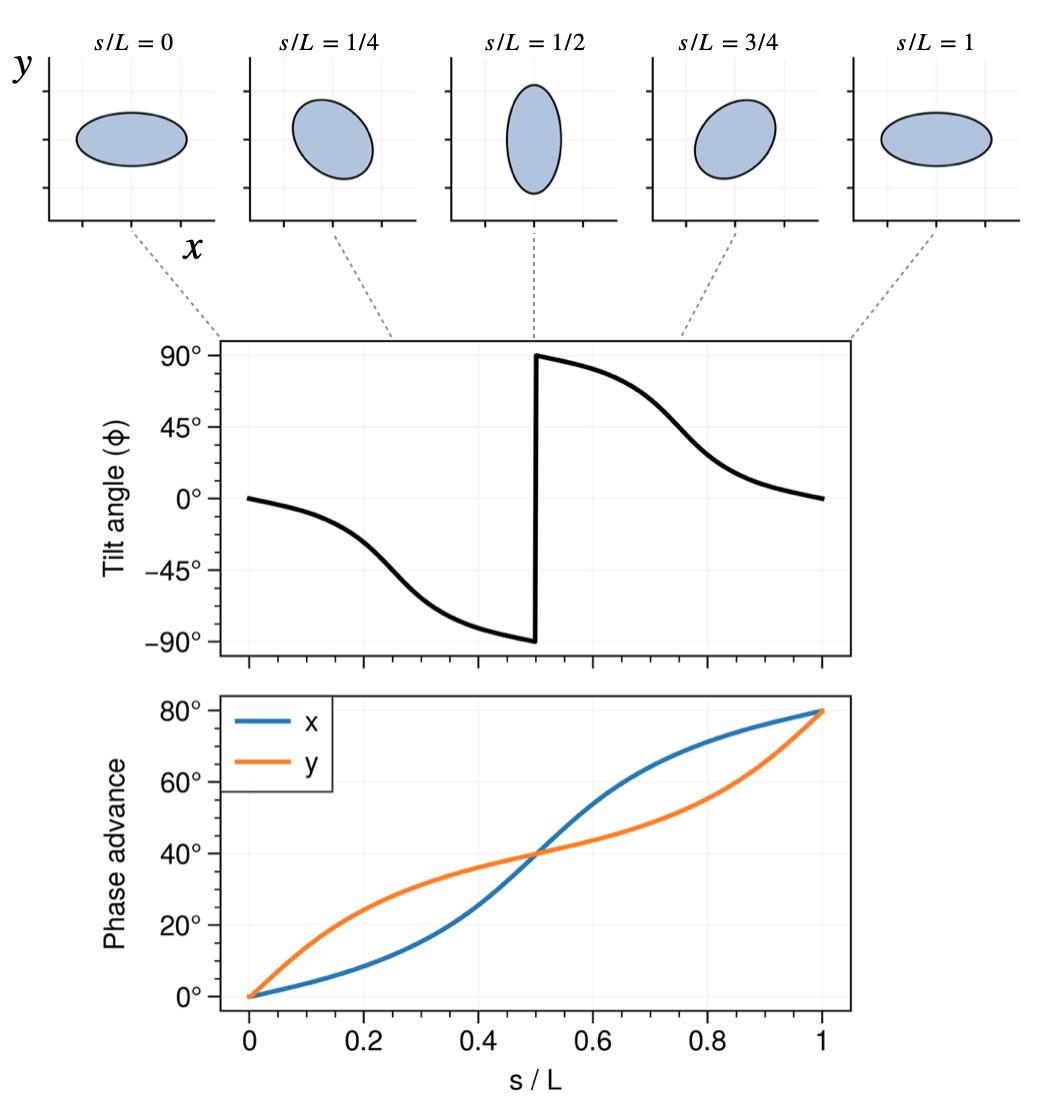
\includegraphics[width=0.8\textwidth]{Images/chapter2/fodo_zerosc.png}
    \caption{Relationship between the tilt angle in real space and the $x$ and $y$ phase advances for a Danilov distribution in a FODO cell of length $L$. The beam is tracked without space charge by integrating the envelope equations.}
    \label{fig:fodo_zerosc}
\end{figure}
%
The tilt angle is a function of the difference between the horizontal and vertical phase advances, which are calculated from
\begin{equation} \label{eq:phase_advance}
    \mu_x(s) = \int_{0}^{s}
    {\frac{\varepsilon_x(s')}{{\tilde{x}(s')}^2} \, ds'},
\end{equation}
where $\tilde{x}^2 = \langle{x^2}\rangle$ and $x$ and $y$ can be interchanged.



\section{Matched envelope computation}

A matched beam in a periodic lattice satisfies 
%
\begin{equation} \label{eq:matched_sigma}
    \bm{\Sigma}(s) = \bm{\Sigma}(s + L)
\end{equation}
%
for all $s$, where $L$ is the period length and $\bm{\Sigma}$ is the covariance matrix. The problem of computing the matched envelope is as follows:
%
\begin{equation}
\begin{aligned}
    & \underset{\bm{\Sigma}}{\text{minimize}}
    & & C(\bm{\Sigma}) = \left\Vert{\mathbf{M} \bm{\Sigma} \mathbf{M}^T - \bm{\Sigma}}\right\Vert^2 \\
    & \text{subject to}
    & & |\bm{\Sigma}| = 0,
\end{aligned}
\end{equation}
%
where $\mathbf{M} = \mathbf{M}(\bm{\Sigma})$ is a linear transfer matrix connecting the initial and final covariance matrix, and $\Vert\dots\Vert$ is the matrix norm. The constraint that the covariance matrix must be singular comes from Eq.~\eqref{eq:mode_emittances2}. Additionally, we would like to hold the nonzero intrinsic emittance fixed so that a unique solution is found for a given lattice and beam perveance. An iterative approach is needed since space charge causes $\mathbf{M}$ to depend on $\bm{\Sigma}$ in a potentially complicated way which is unknown before tracking the beam. 


\subsection{Motivation}

The calculation of the matched beam envelope is of practical importance for space charge dominated beams; it is a common first step in lattice design \cite{Lund2006}. The amount of beam current able to be transported through a periodic focusing channel with a given aperture is maximum when the beam is matched \cite{book:Reiser}. The matched beam is the minimum energy solution, and the free energy available in a mismatched beam may result in emittance growth and halo formation \cite{book:Reiser}. Calculation of the matched envelope is generally the first step in a stability analysis of the envelope equations. The task has been performed for the KV distribution in both uncoupled and coupled focusing systems \cite{Hofmann1983, Chernin1988, Ryne1995, Lund2006, Anderson2007, Goswami2016}. 

The purpose of this section is to calculate and describe the properties of the matched envelope of the Danilov distribution in simple focusing systems as space charge is increased. A better understanding of the coupled beam dynamics under the influence of external and internal forces should fall out of this analysis, as well as the ability to calculate the matched envelope in more complicated focusing systems. The relevance to SNS experiments that seek to paint the Danilov distribution is clear: the painting method only works as intended if the circulating beam is matched.

Before presenting our solution, we highlight the space-charge-driven mismatch oscillations that are to be corrected. Fig.~\ref{fig:fodo_mismatch_tbt} shows the turn-by-turn evolution of a beam that is matched to a lattice without space charge and then tracked with space charge. 
%
% \begin{figure}[!p]
%     \centering
%     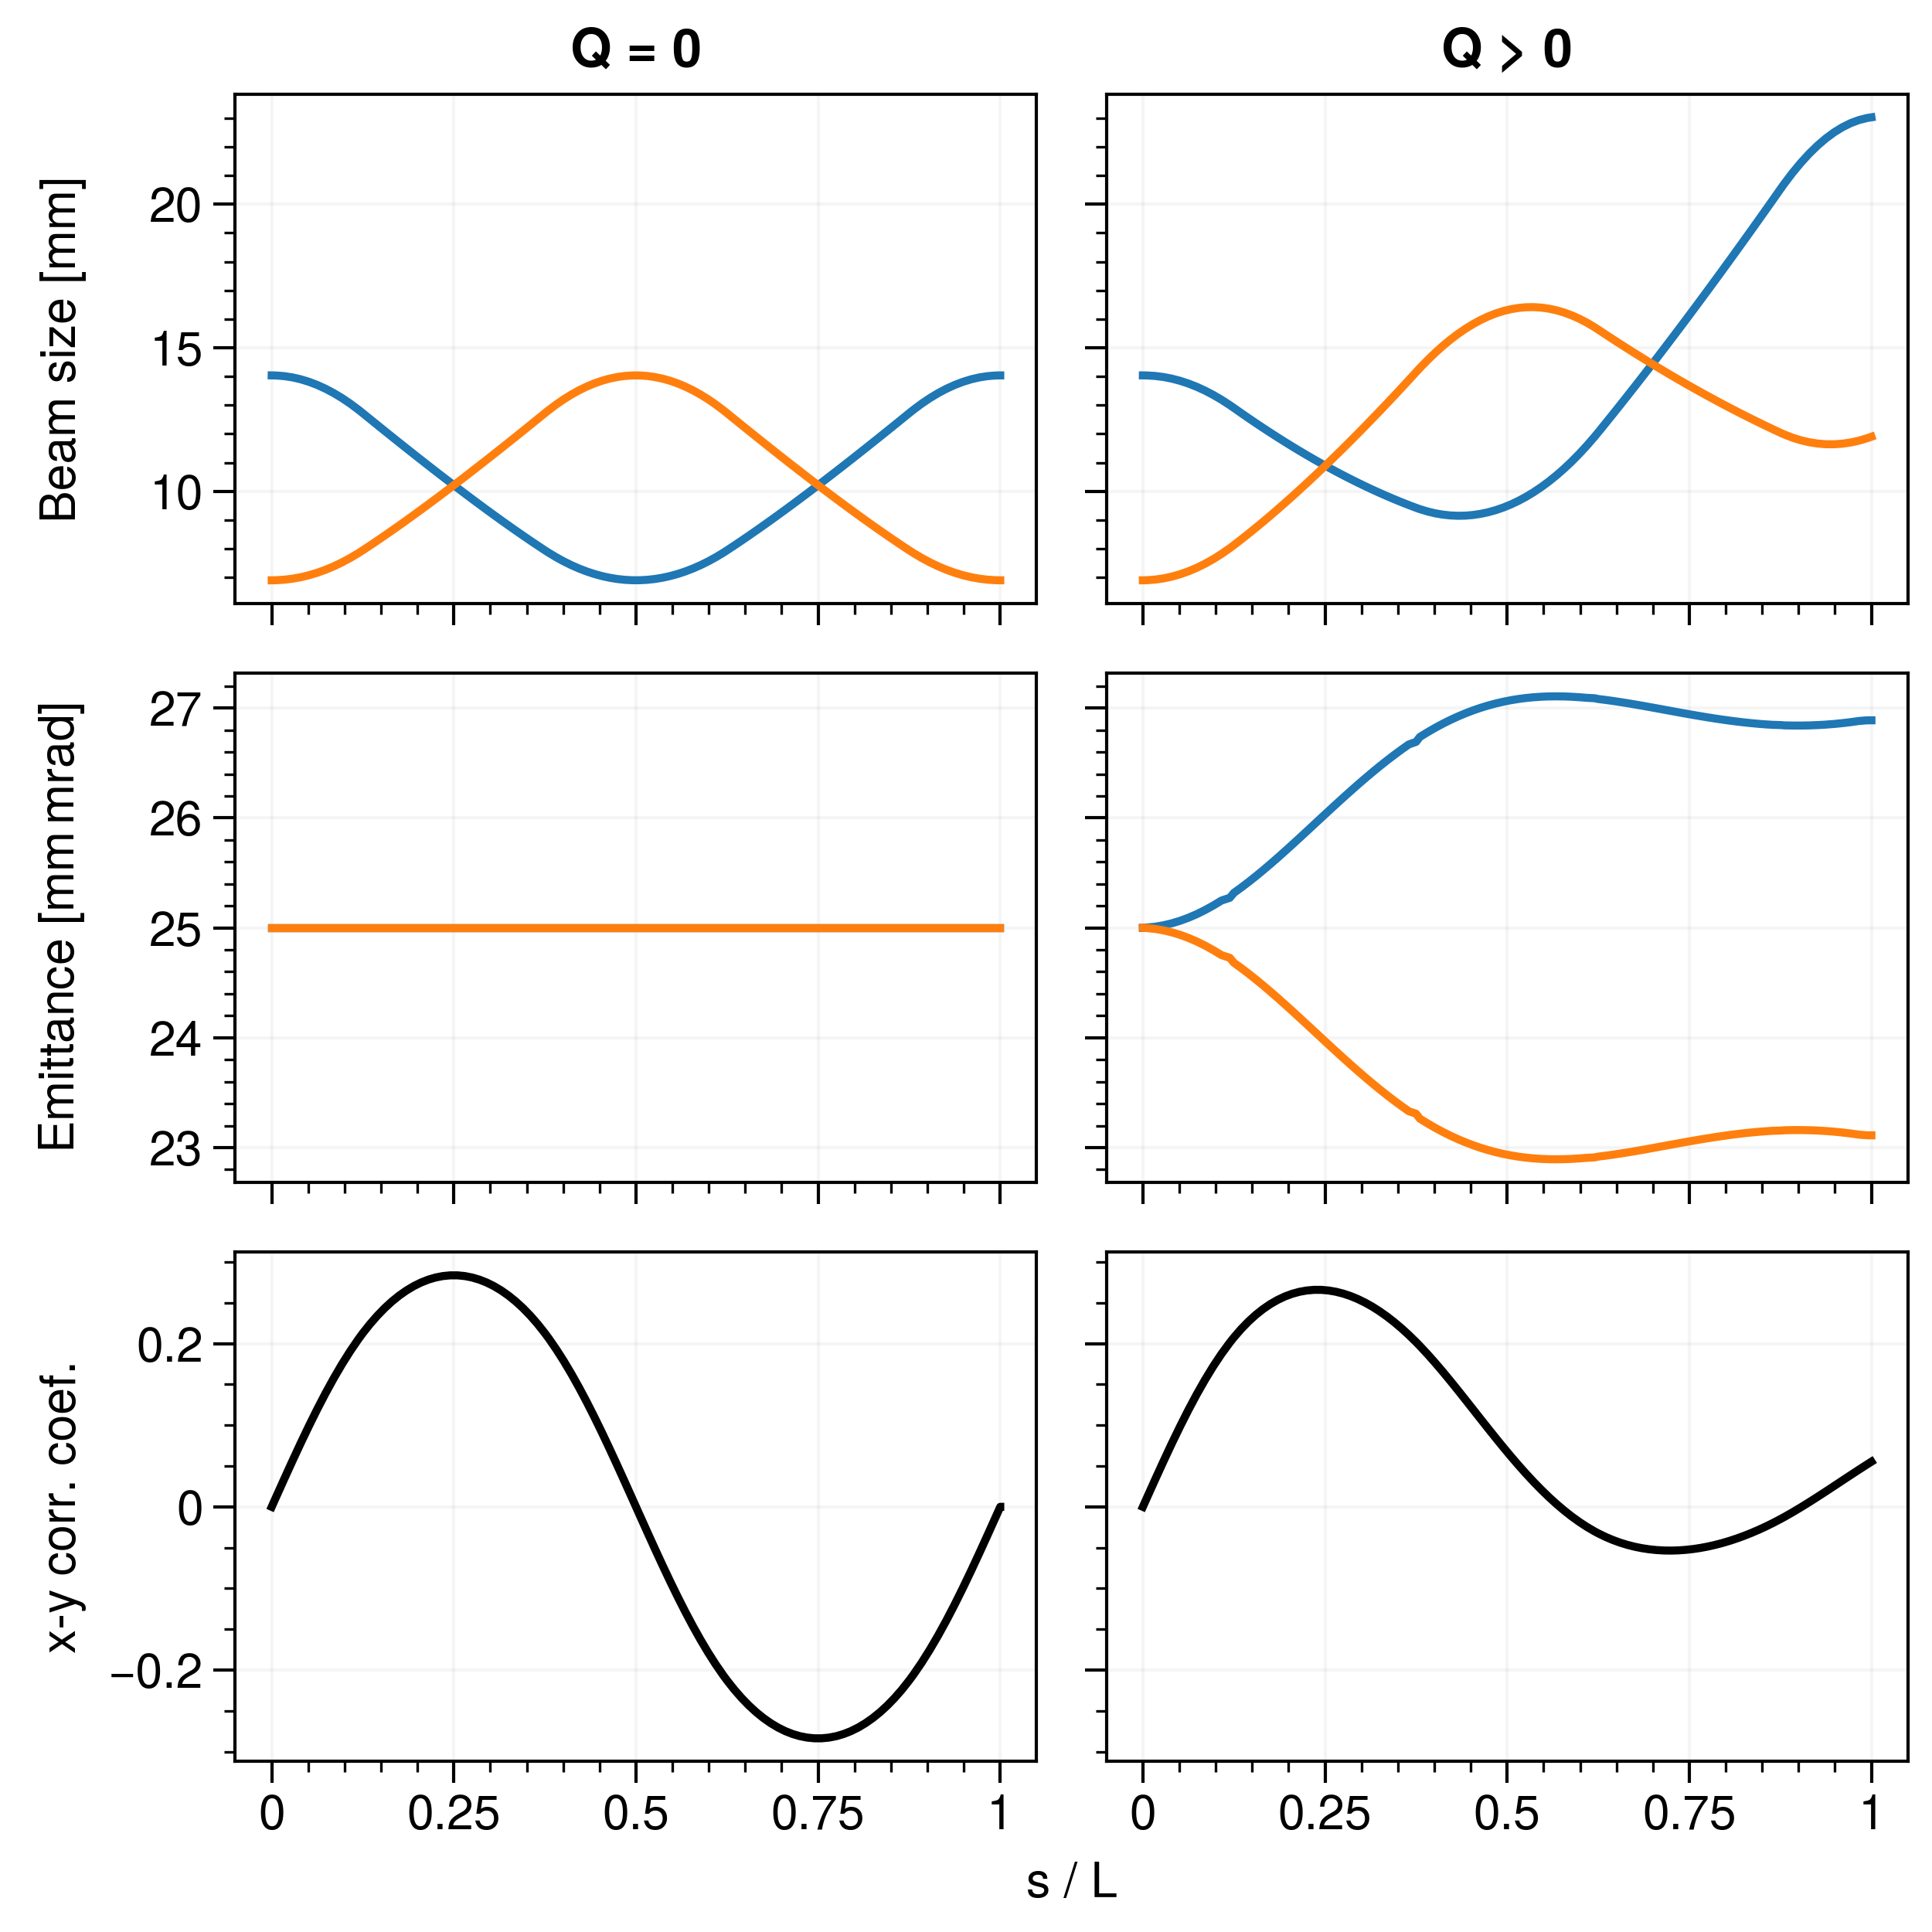
\includegraphics[width=0.8\textwidth]{Images/chapter2/fodo_mismatch_withinlattice.png}
%     \caption{Evolution of the Danilov distribution within an uncoupled FODO lattice of period length $L$ without space charge (left) and with space charge (right). Blue (orange) corresponds to the $x$ ($y$).}
%     \label{fig:fodo_mismatch_withinlattice}
% \end{figure}
%
\begin{figure}[!p]
    \centering
    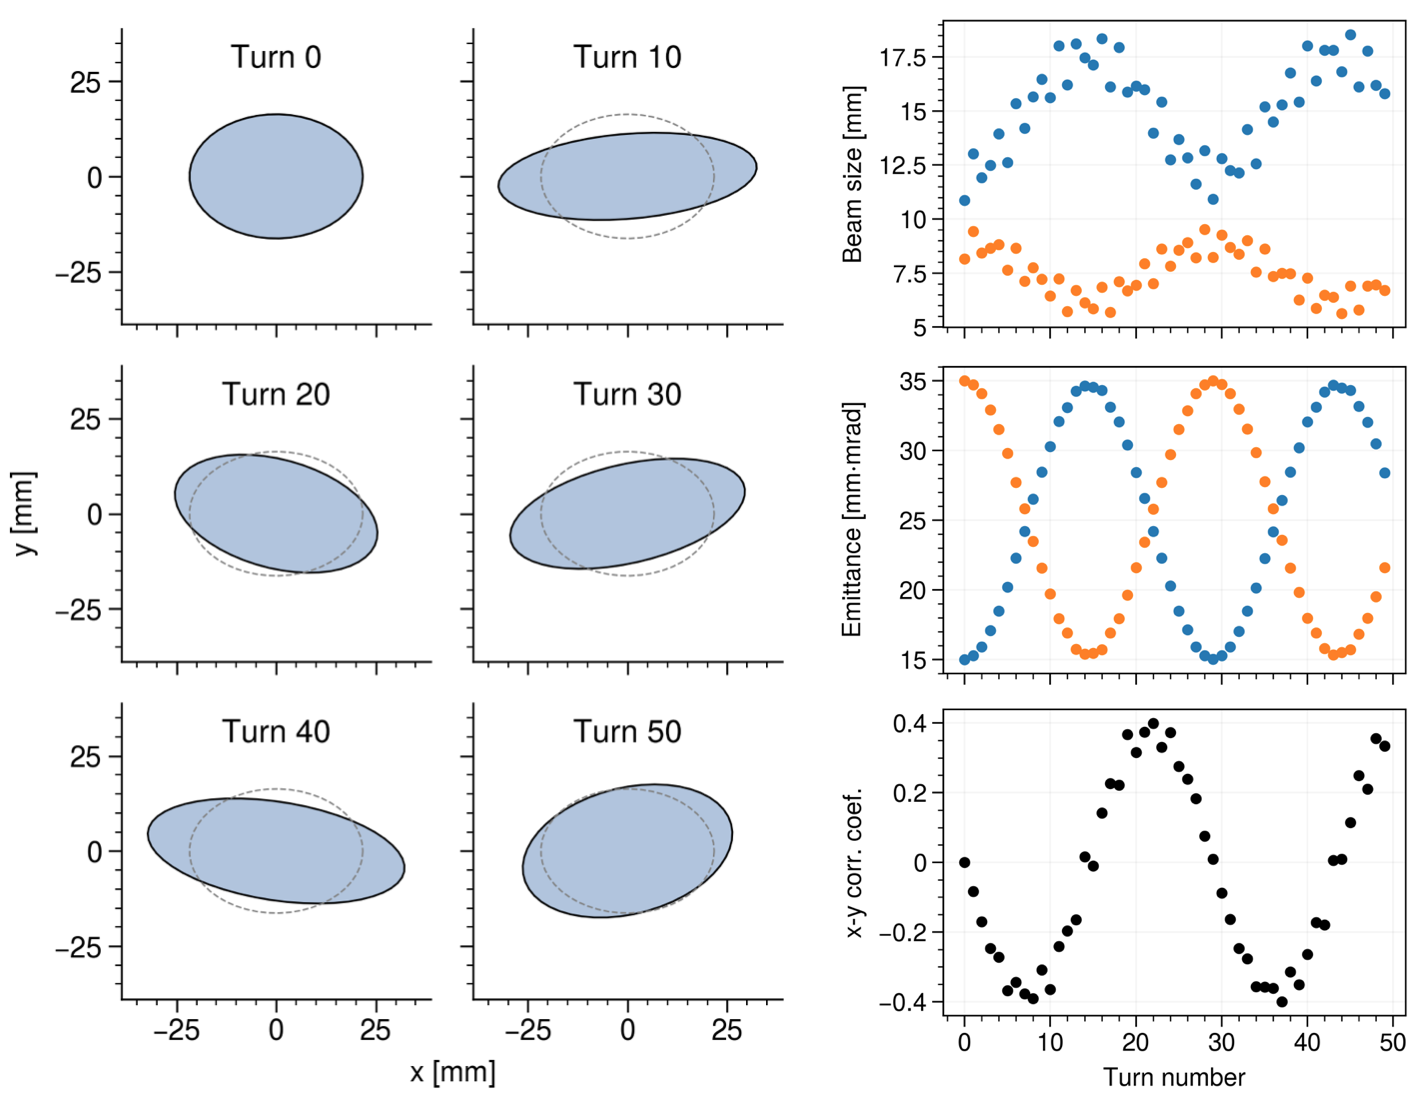
\includegraphics[width=\textwidth]{Images/chapter2/fodo_mismatch_tbt.png}
    \caption{Turn-by-turn mismatch oscillations of the Danilov distribution at the entrance of an uncoupled FODO lattice. The beam would be matched to the lattice without space charge. In the right column, blue (orange) corresponds to $x$ ($y$).}
    \label{fig:fodo_mismatch_tbt}
\end{figure}
%
There are two frequencies in the mismatch oscillations: a larger frequency near twice the zero-current tune corresponding to the breathing oscillation of the beam sizes, and a smaller frequency corresponding to the emittance exchange from space-charge-driven linear coupling. 


\subsection{Solution}

The problem of computing the matched envelope can be approached in the following way. The effect of space charge is to modify the linear focusing strength at every position; we call this modified focusing system the \textit{effective lattice}. Generating a beam that is matched to the lattice with space charge is equivalent to generating a beam that is matched to the effective lattice without space charge. The latter task is straightforward using an existing parameterization of coupled motion. The correct effective lattice is of course unknown a priori, so a search must be performed over the lattice parameters. Fig.~\ref{fig:effective_lattice} illustrates the concept of the effective lattice.
%
\begin{figure}
    \centering
    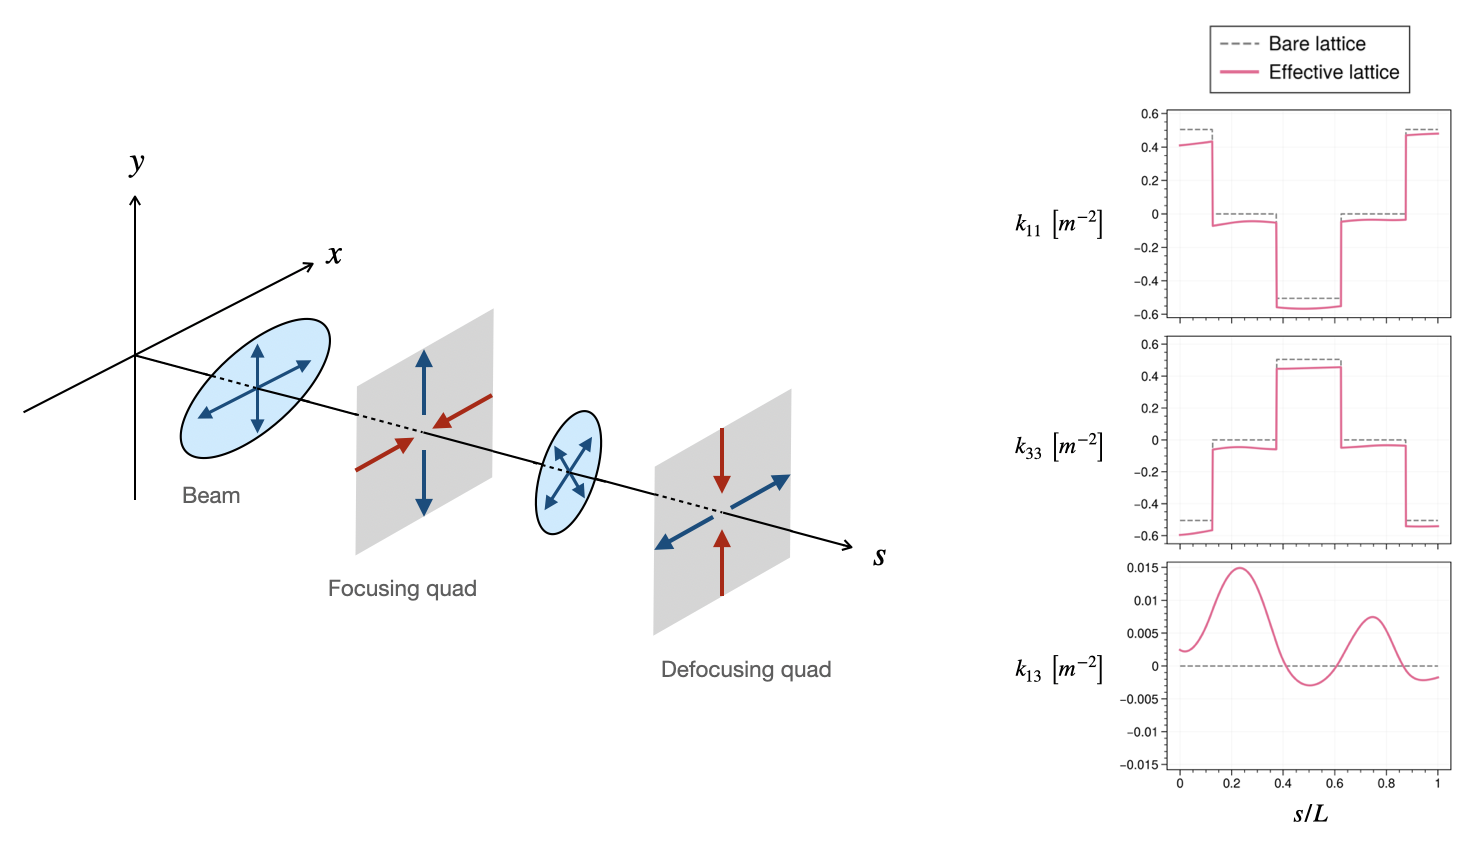
\includegraphics[width=1.0\textwidth]{Images/chapter2/effective_lattice.png}
    \caption{Illustration of the effective lattice — the net linear focusing after space charge is included. The coefficients $k_{ij}$ are defined in Eq.~\eqref{eq:single_particle_eom_coupled}.}
    \label{fig:effective_lattice}
\end{figure}
%

\subsubsection{Zero space charge}

We begin by demonstrating how to compute the matched envelope without space charge. We write Eq.~\eqref{eq:eigvec_coords} again for convenience:
%
\begin{equation}
    \mathbf{Mx} = Re \left\{
        \sqrt{2 J_1} \, \mathbf{v}_1 \, e^{-i(\psi_1 + \mu_1)}
        + \sqrt{2 J_2} \, \mathbf{v}_2 \, e^{-i(\psi_2 + \mu_2)}
    \right\}.
\end{equation}
%
The turn-by-turn trajectory of a particle with a given $J_{1,2}$ forms a closed surface in phase space, and a group of particles distributed uniformly over this surface will appear to be invariant. A matched distribution can be thought of as a collection of these surfaces with different amplitudes.

We now switch to the collective description of the beam using its covariance matrix. The symplectic normalization matrix $\mathbf{V}$ (from Eq.~\eqref{eq:V_from_eigvecs}) can be used to express the matched beam covariance matrix as
%
\begin{equation}\label{eq:sigma_n}
    \bm{\Sigma}_n = 
    \mathbf{V}
    \begin{bmatrix}
        \varepsilon_1 & 0 & 0 & 0 \\
        0& \varepsilon_1 & 0 & 0 \\
        0 & 0 & \varepsilon_2 & 0 \\
        0 & 0 & 0 & \varepsilon_2
    \end{bmatrix}
    \mathbf{V}^T.
\end{equation}
%
In the uncoupled case, $\mathbf{V}^{-1}$ transforms a tilted ellipse in the $x$-$x'$ plane into a circle. In the coupled case, $\mathbf{V}^{-1}$ transforms a ``tilted" 4D ellipsoid into an ``upright" 4D ellipsoid.

A parameterization of $\mathbf{V}$ was introduced in Fig.~\ref{fig:twiss4D}. The number of parameters can be reduced to six by observing that the Danilov distribution is a function of only one eigenvector. We now set one of the intrinsic emittances to zero in Eq.~\eqref{eq:sigma_n} and display the connection between the parameters and the covariance matrix. The beta functions $\beta_{lx}$ and $\beta_{ly}$ give the ratios between the beam size and intrinsic emittance:
%
\begin{equation}
    \beta_{lx} = \frac{\langle{x^2}\rangle}{\varepsilon_l}, \quad
    \beta_{ly} = \frac{\langle{y^2}\rangle}{\varepsilon_l}
\end{equation}
%
where again $l = 1$ or $2$. Similarly, the alpha functions $\alpha_{lx}$, and $\alpha_{ly}$ give the ratios between the beam divergence and the intrinsic emittance:
%
\begin{equation}
    \alpha_{lx} = -\frac{\langle{xx'}\rangle}{\varepsilon_l}, \quad
    \alpha_{ly} = -\frac{\langle{yy'}\rangle}{\varepsilon_l}
\end{equation}
%
Next, $u$ gives the ratio between the apparent emittance and the intrinsic emittance. When $l = 1$:
%
\begin{equation} \label{eq:u}
     u = \frac{\varepsilon_y}{\varepsilon_1},
\end{equation}
%
or when $l = 2$:
%
\begin{equation}
     u = \frac{\varepsilon_x}{\varepsilon_2}.
\end{equation}
%
Finally, $\nu_l$, is directly related to the $x$-$y$ correlation coefficient:
%
\begin{equation}
    \cos\nu_l = \frac{\langle{xy}\rangle}{\sqrt{\langle{x^2}\rangle\langle{y^2}\rangle}}.
\end{equation}
%
The subscript will be dropped from now on since it has no effect. As mentioned in Fig.~\ref{fig:fodo_zerosc}, $\nu$ will vary even without the presence of coupled forces. For example, Fig.~\ref{fig:splittunes_tbt} shows the turn-by-turn $x$-$y$ projection of a beam whose $x$-$x'$ and $y$-$y'$ ellipses are matched to an uncoupled lattice with a tune separation of 0.01, along with the value of $\nu$ at each frame. 
%
\begin{figure}[!p]
    \centering
    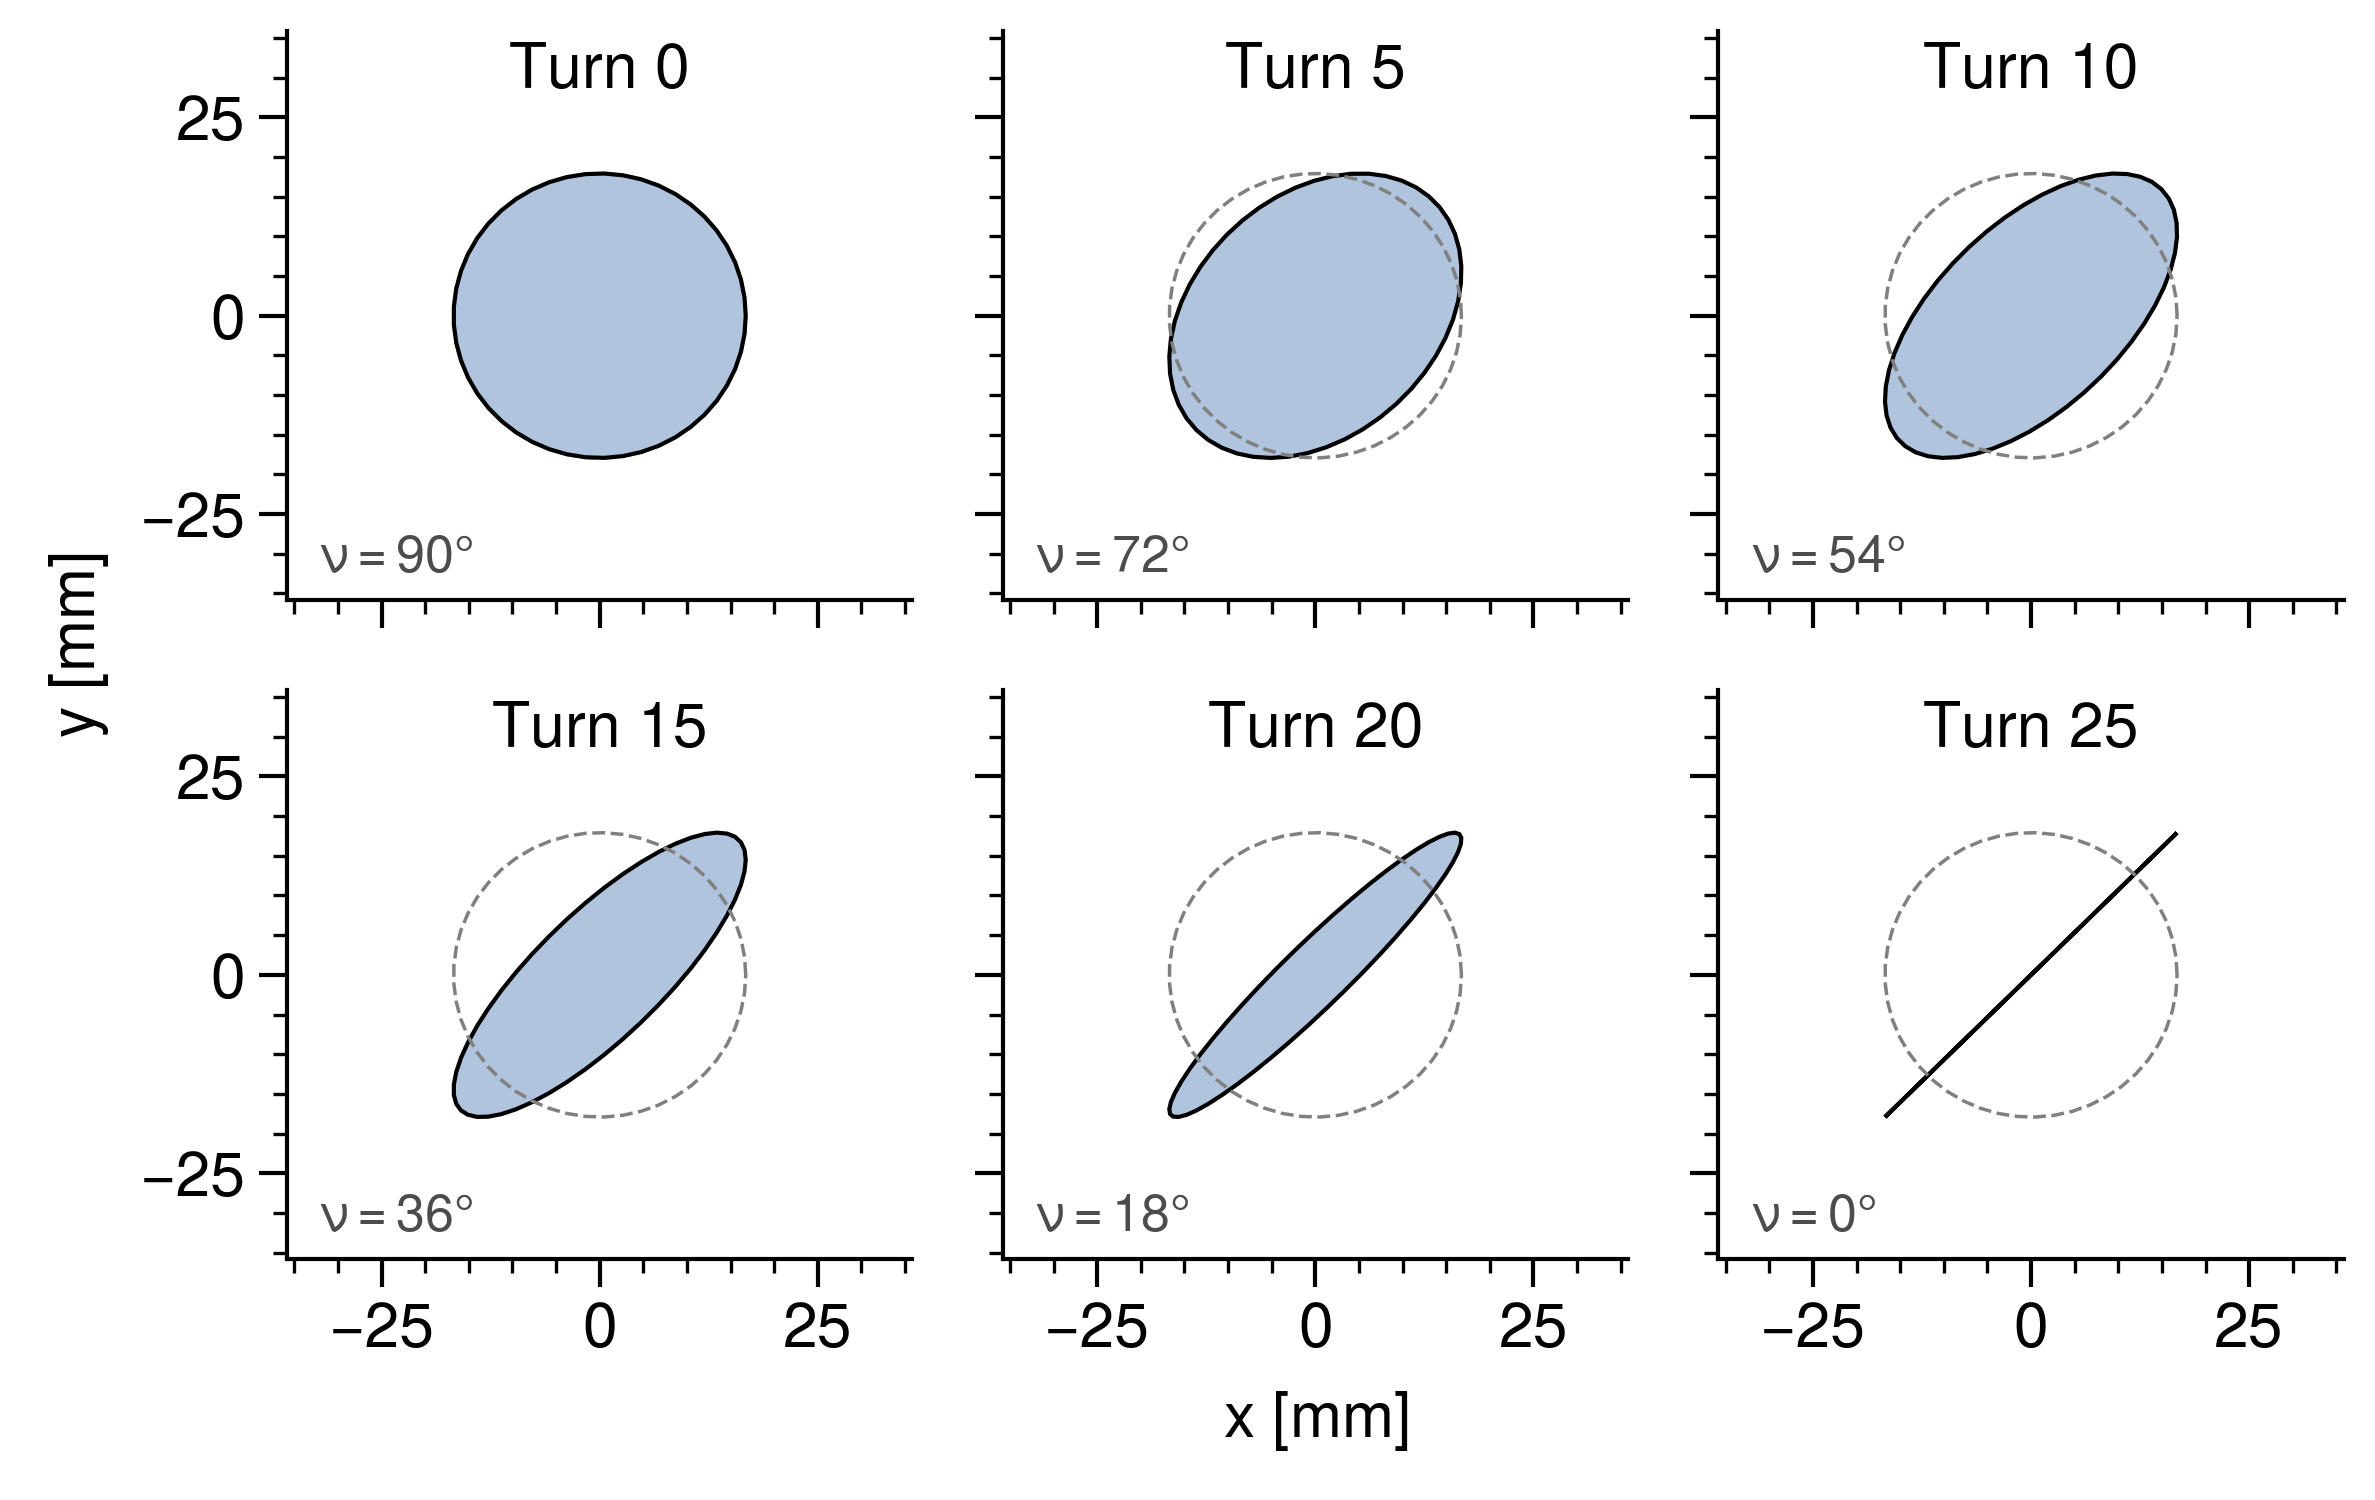
\includegraphics[width=0.8\textwidth]{Images/chapter2/splittunes_tbt.png}
    \caption{Turn-by-turn $x$-$y$ projections of a Danilov distribution in a lattice with a tune split of 0.01. The horizontal and vertical phase space projections are matched to the lattice.}
    \label{fig:splittunes_tbt}
\end{figure}
%

In summary, the matched beam is described by a vector of parameters $\mathbf{p}$, where
%
\begin{equation} \label{eq:twiss_params_4D}
    \mathbf{p} = (\alpha_{lx}, \alpha_{ly}, \beta_{lx}, \beta_{ly}, u, \nu)
\end{equation}
%
with $l = 1$ or $2$ depending on which intrinsic emittance is zero.



\subsubsection{Nonzero space charge}

We denote the choice $\varepsilon_2 = 0$ as solution $1$ and $\varepsilon_1 = 0$ as solution 2. Once this emittance is chosen, $p$ is initialized using the bare lattice parameters. We then perform the following procedure:
%
\begin{enumerate}
  \item Generate a beam envelope from $\mathbf{p}$.
  \item Track the beam through one lattice period and compute the cost function.
  \item Update $\mathbf{p}$.
  \item Stop if the relative change in $C$ or $|\mathbf{p}|$ is below a given tolerance, otherwise repeat from step 1.
\end{enumerate}
%
A trust-region minimization algorithm \cite{Branch1999} is used to determine the update strategy for $\mathbf{p}$. If necessary, the process can be repeated at multiple steps so that the seed envelope remains close to the matched solution. In one case during our studies, this optimizer failed to converge and it became necessary to use a custom update method; in this method, the beam is tracked for a number of turns and $\mathbf{p}$ is updated to the average of its average over those turns. The method does not need to worry about bounds on the parameters since every update is based on an already existing beam. An example of the progress of this method over the first few iterations is shown in Fig.~\ref{fig:optimizer_iters}. 

\begin{figure}[!p]
    \centering
    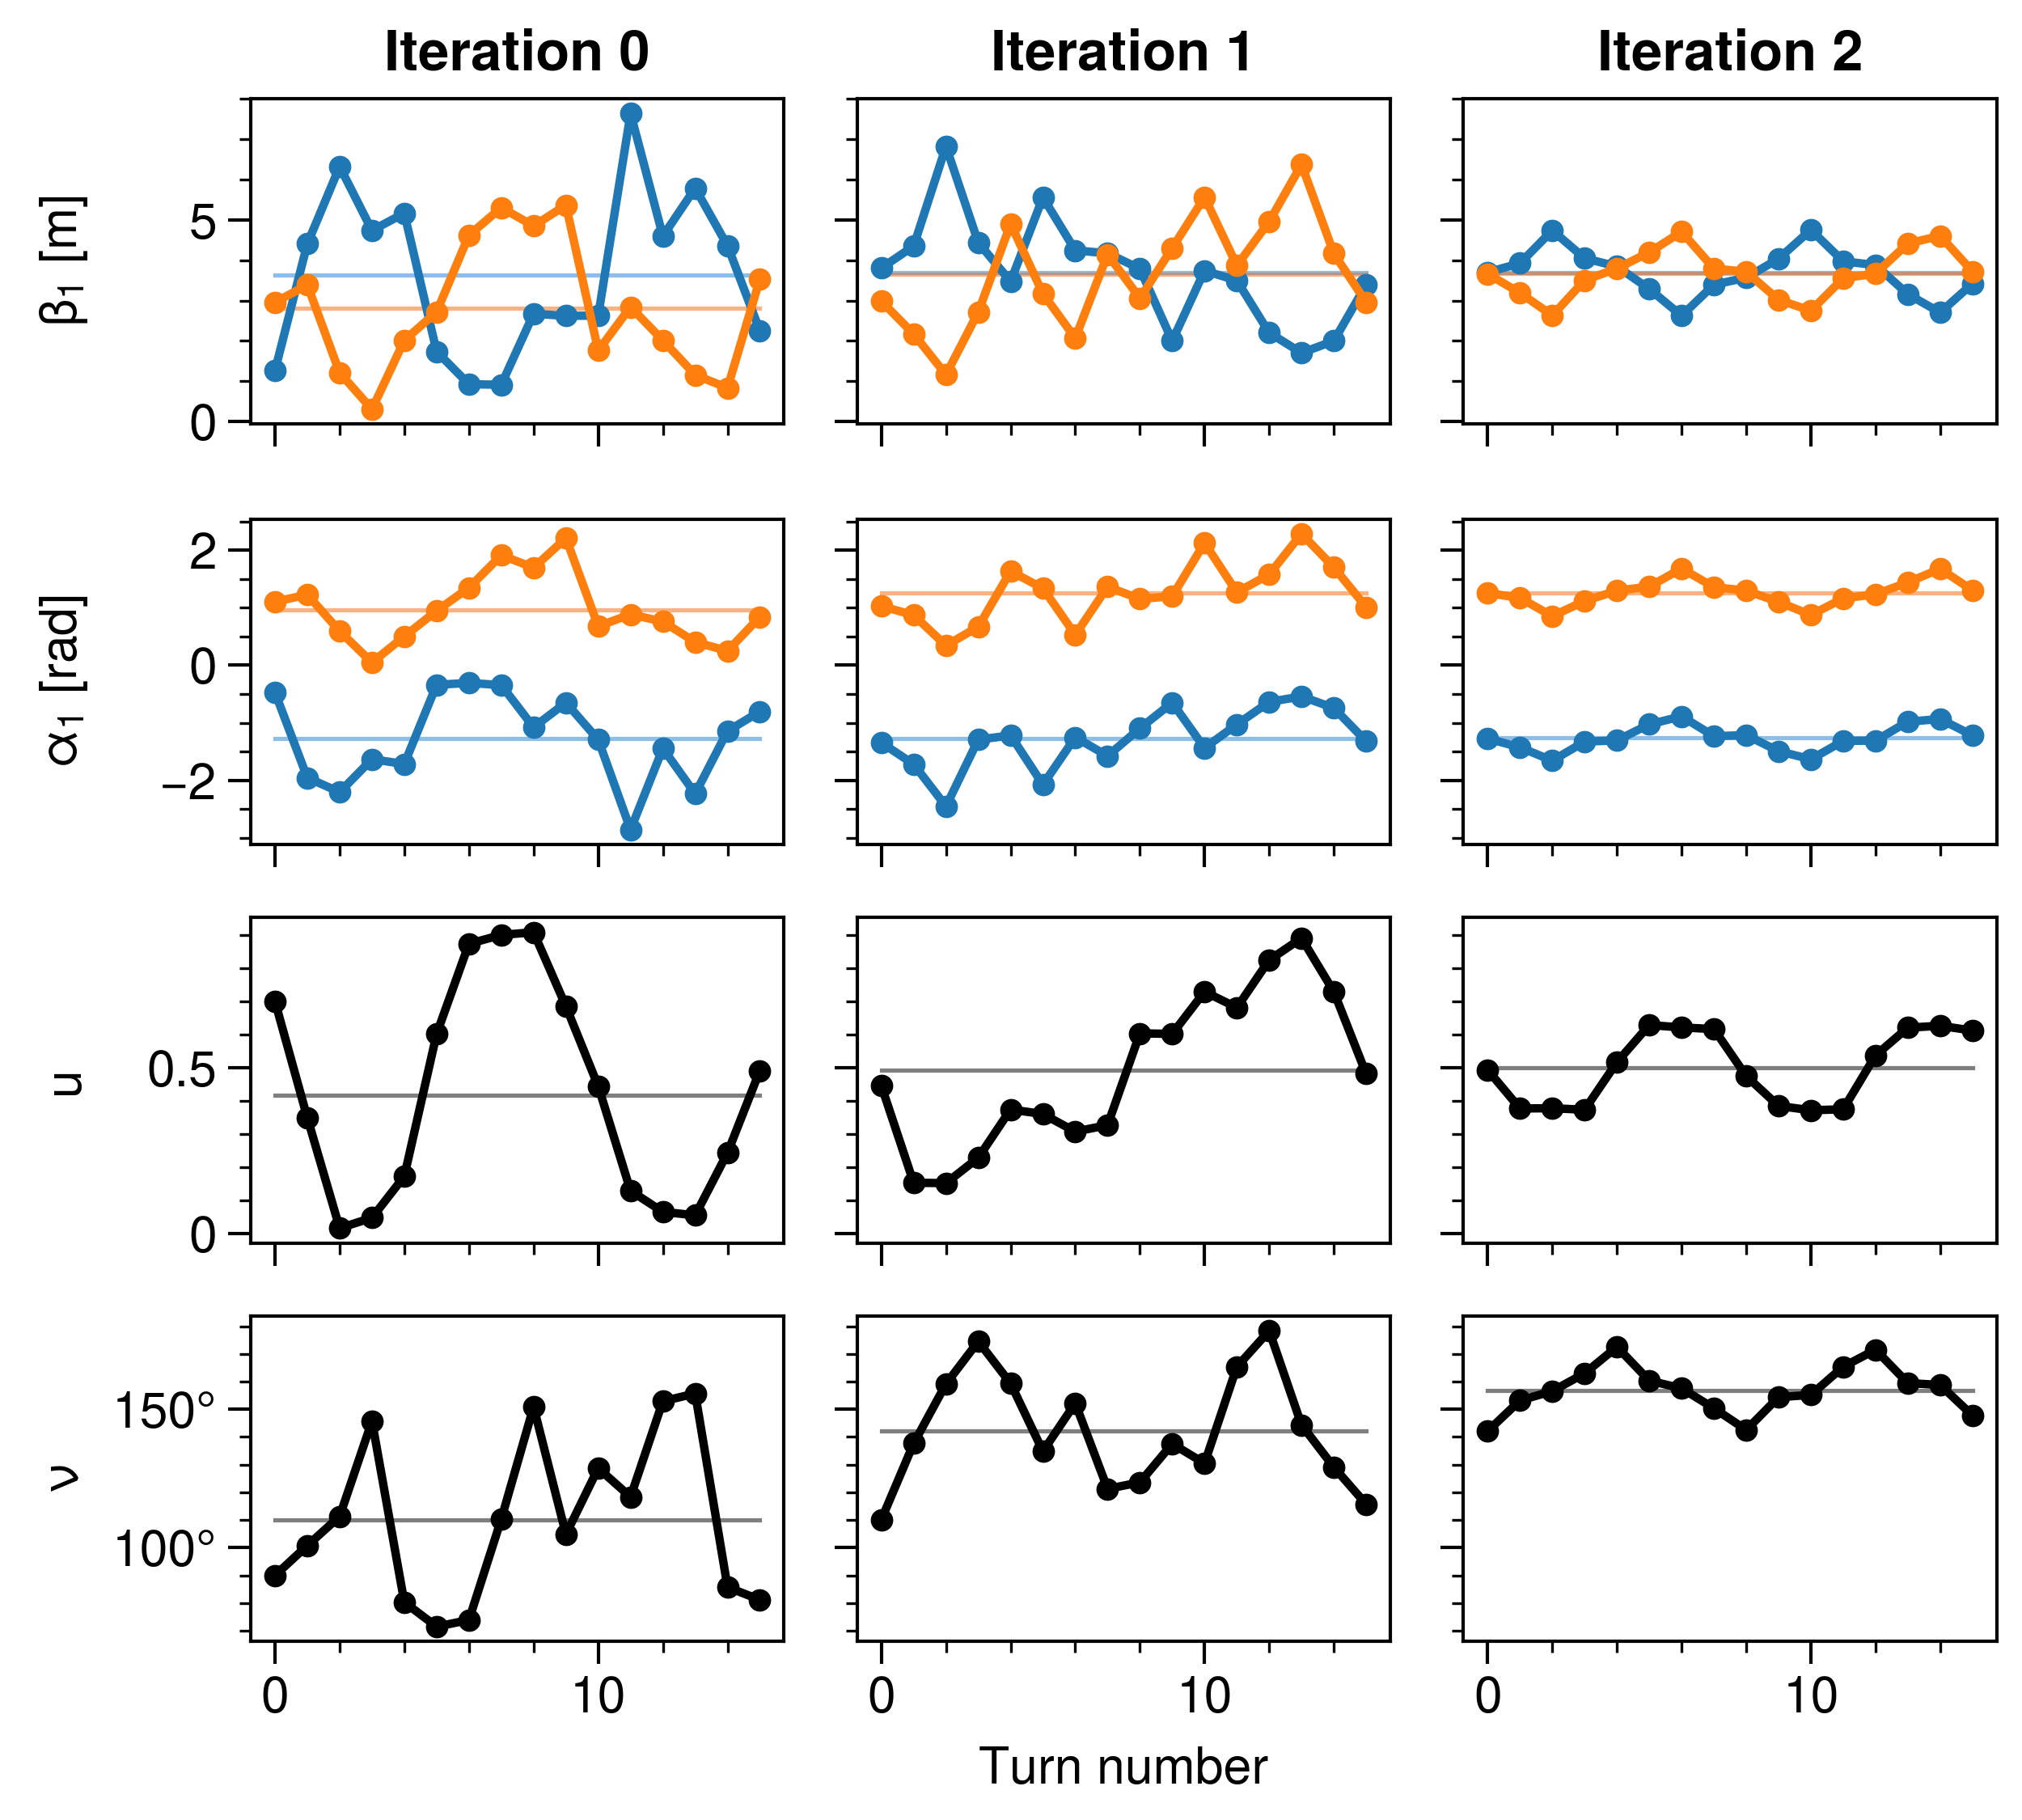
\includegraphics[width=0.8\textwidth]{Images/chapter2/optimizer_iters.png}
    \caption{Turn-by-turn oscillations of the beam parameters after the first few iterations of the matching routine. The custom update method is used. Faint horizontal lines give the average of the oscillations. Blue (orange) corresponds to $x$ ($y$).}
    \label{fig:optimizer_iters}
\end{figure}








\subsection{Method demonstration}

The matching routine was applied to an equally spaced, periodic quadrupole (FODO) lattice. The horizontal focusing strength in this lattice is shown in Fig.~\ref{fig:fodo_lattices}a as a function of $s$. Several variants of the FODO lattice were also considered to include external coupling. In Fig.~\ref{fig:fodo_lattices}b, the focusing and defocusing quadrupoles are rotated by $3\degree$ in opposite directions in the transverse plane. In Fig.~\ref{fig:fodo_lattices}c solenoid magnets are inserted in the drift spaces between the quadrupoles. This section examines the matched solutions in each lattice as space charge is increased. Previous studies indicate that the KV envelope equations have a unique matched solution for each choice of lattice, beam perveance, and apparent emittances. Although there is no known proof of this conjecture, it seems to be true based on numerical evidence \cite{Lund2006}. Thus, for the Danilov distribution, it is expected that each choice of lattice and perveance will lead to two matched solutions depending on which intrinsic emittance is set to zero. No evidence to the contrary was found.
%
\begin{figure}[!p]
    \centering
    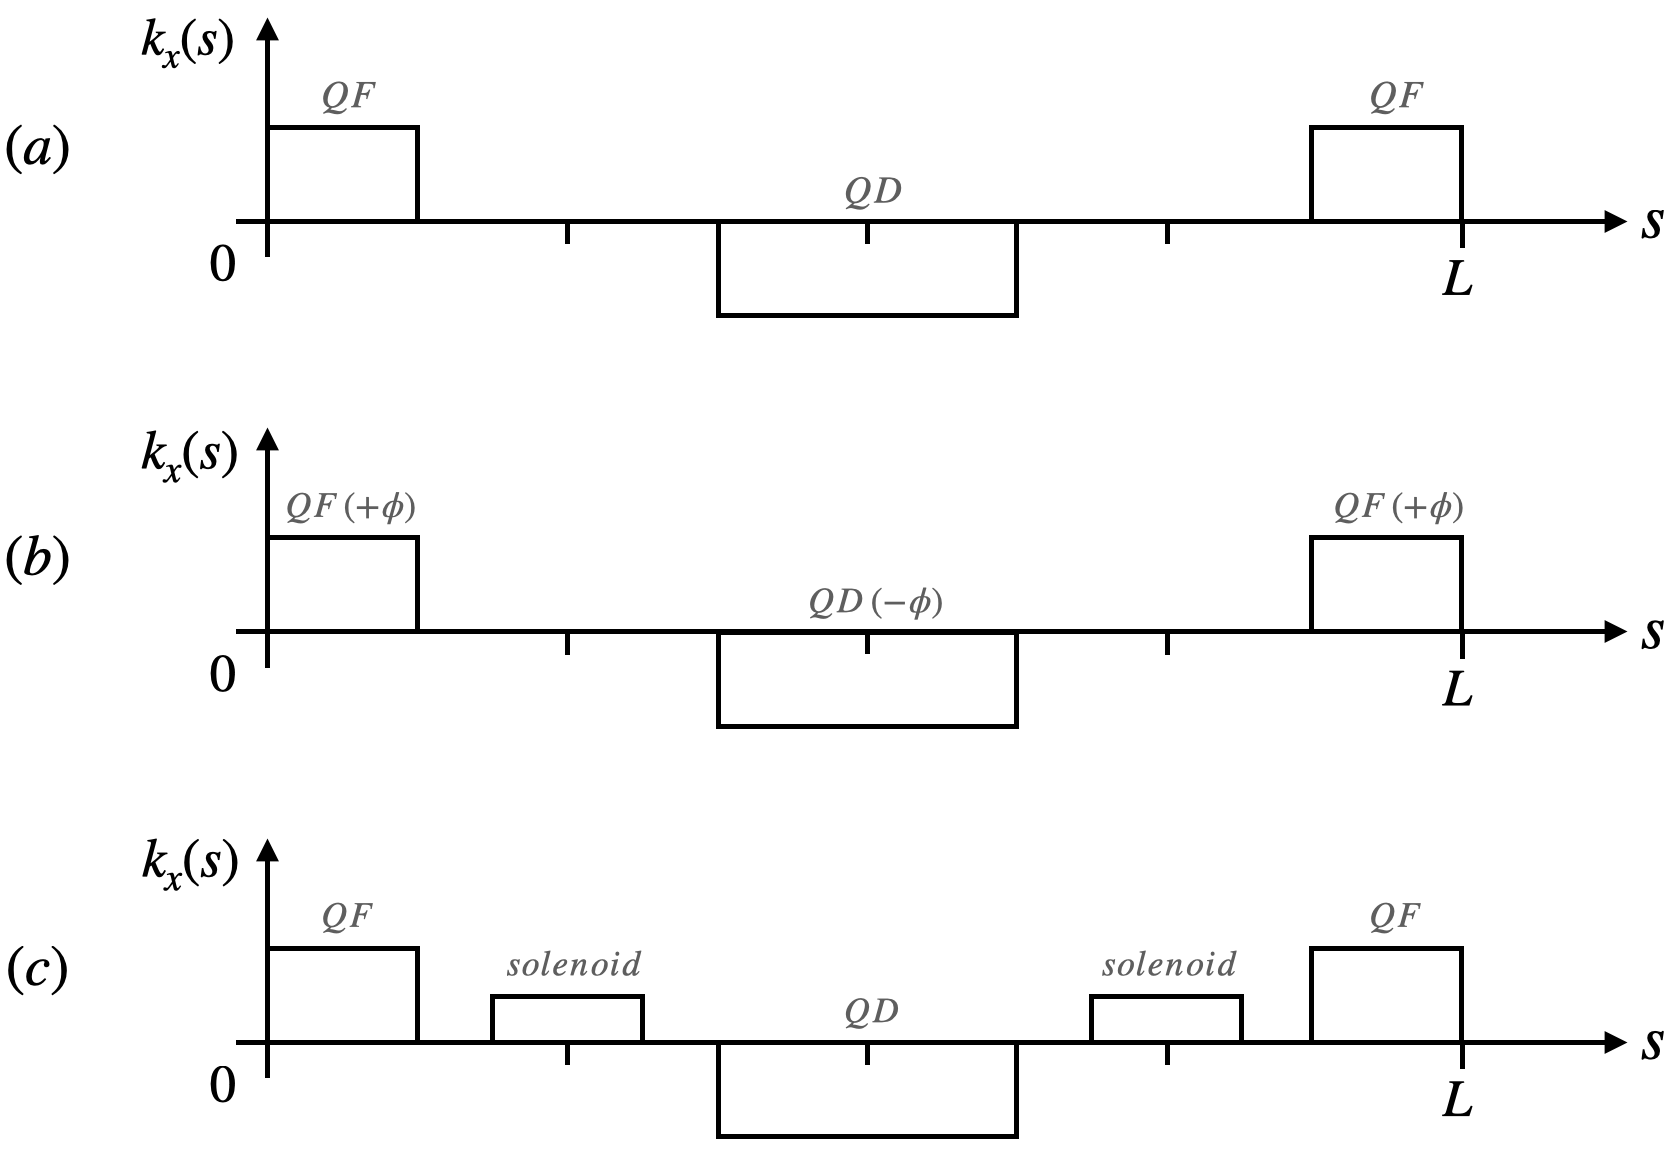
\includegraphics[width=0.8\textwidth]{Images/chapter2/fodo_lattices.png}
    \caption{Horizontal focusing strength as a function of $s$ in a FODO lattice with period length $L$. Quadrupoles have length $L/4$ and are equally spaced. (a) Upright quadrupoles with $80\degree$ phase advance in both planes. (b) The quadrupoles are rotated by $\phi = 3\degree$ in the transverse plane ($QF$ and $QD$ are rotated in opposite directions). (c) Solenoid magnets are inserted between the quadrupoles in (a).}
    \label{fig:fodo_lattices}
\end{figure}


\subsubsection{Uncoupled lattice}

We first present the results for an uncoupled FODO lattice. Fig.~\ref{fig:matched_vs_sc_fodo} shows the matched beam sizes, apparent emittances, and $\nu$ parameter within the lattice for a range of linearly increasing space charge strengths.
%
\begin{figure}[!p]
    \begin{subfigure}{1.0\textwidth}
        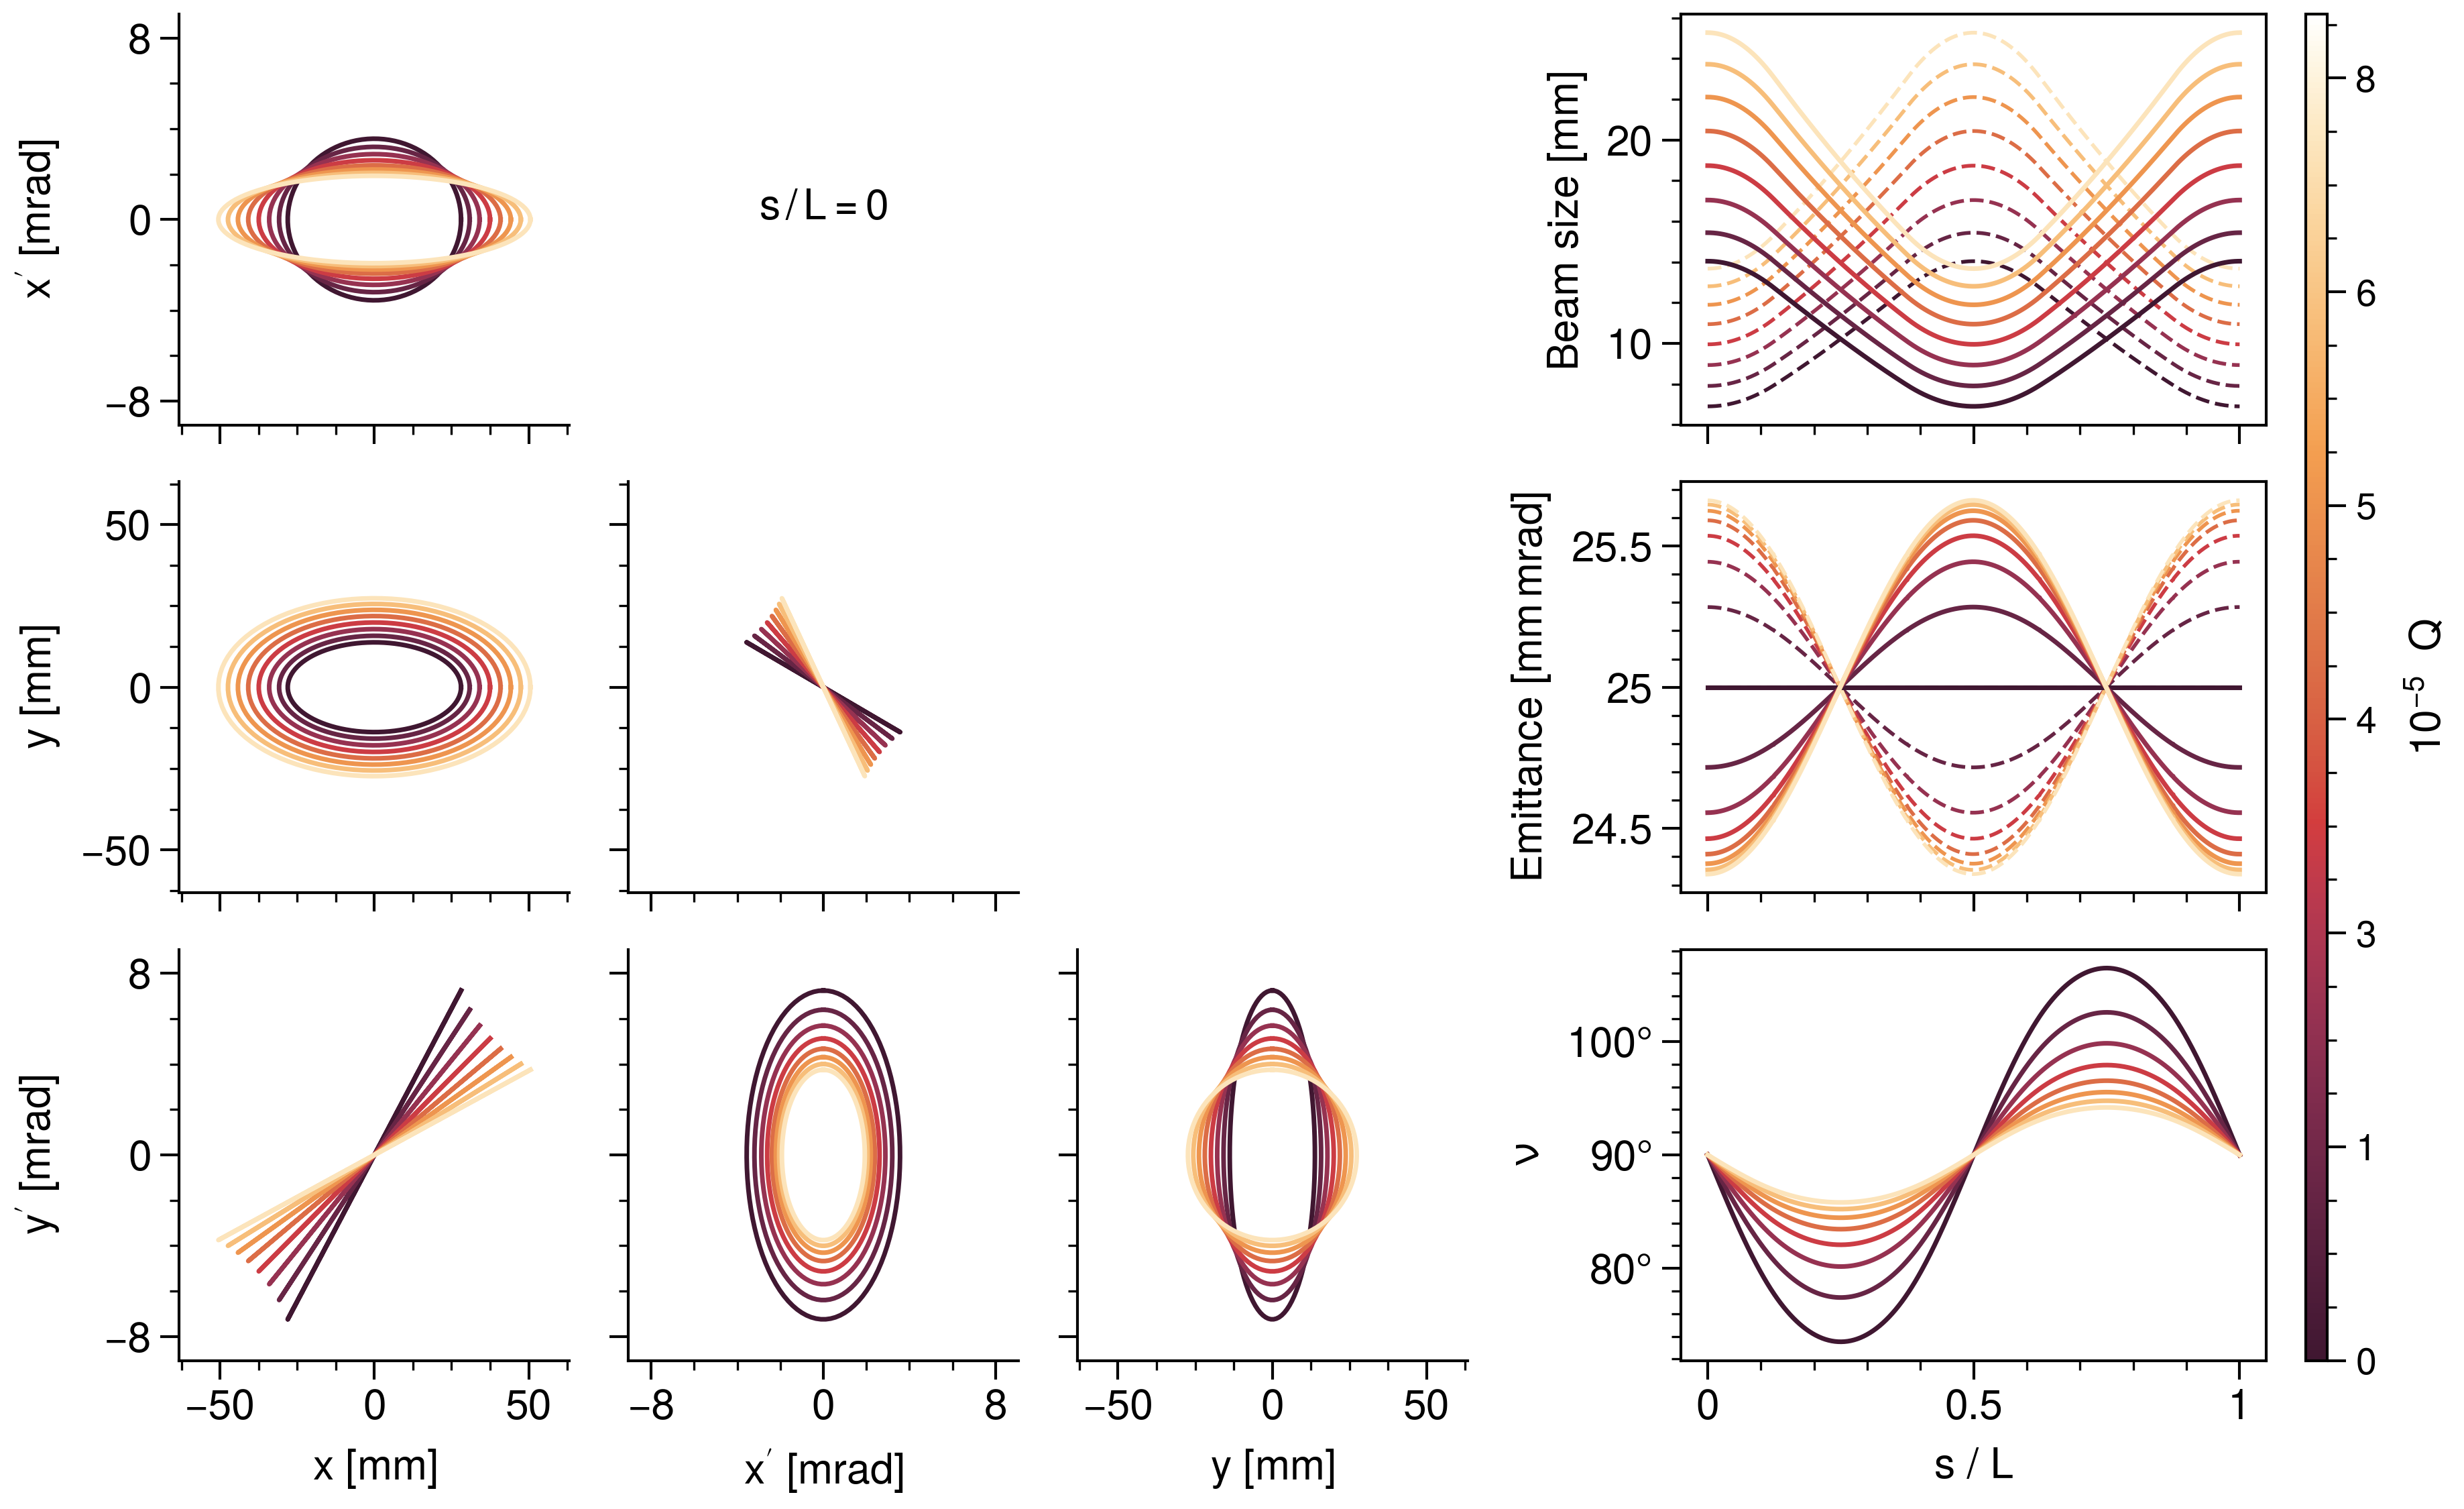
\includegraphics[width=\textwidth]{Images/chapter2/matched_vs_sc_fodo_mode1.png}
        \caption{Solution 1}
        \label{fig:matched_vs_sc_fodo_a}
    \end{subfigure}
    \vfill
    % \vspace*{1.0cm}
    \vfill
    \begin{subfigure}{1.0\textwidth}
        \centering
        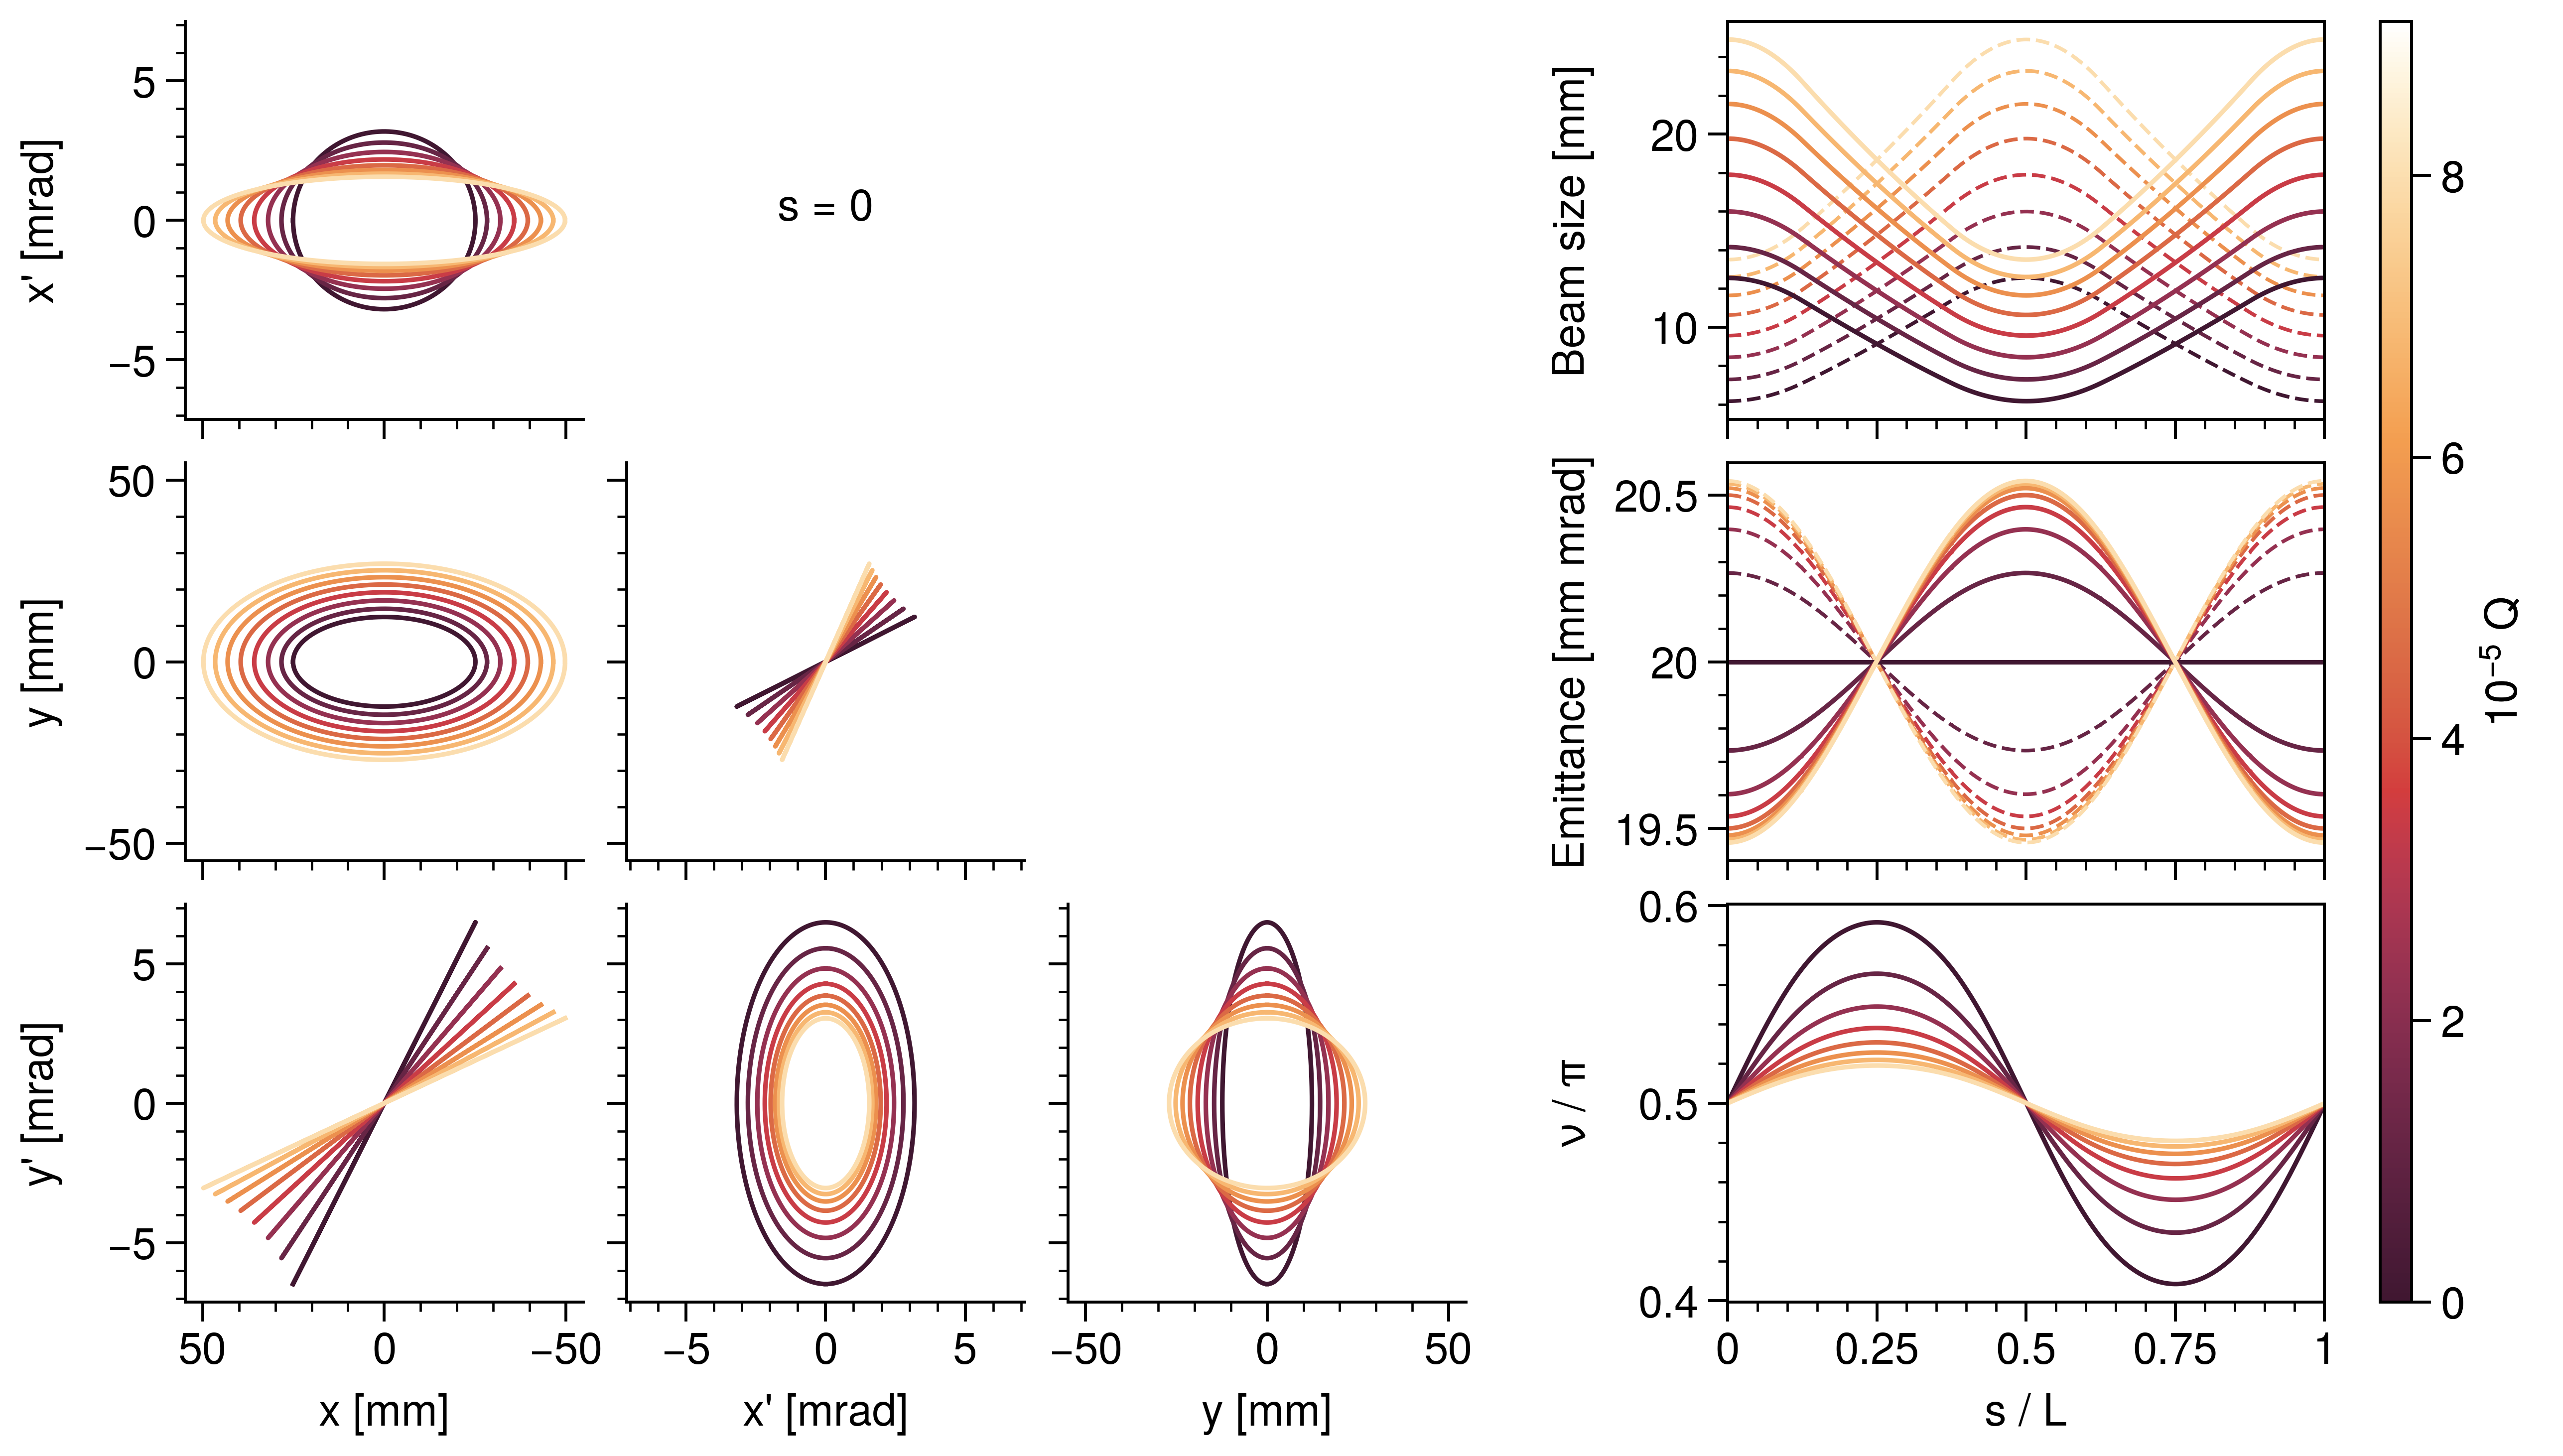
\includegraphics[width=\textwidth]{Images/chapter2/matched_vs_sc_fodo_mode2.png}
        \caption{Solution 2}
        \label{fig:matched_vs_sc_fodo_b}
    \end{subfigure}
    \caption{Matched envelope of the Danilov distribution in an uncoupled FODO lattice as space charge is increased. Left: phase space projections at the lattice entrance. Right: beam parameters within the lattice. Solid lines are for $x$ and dashed lines are for $y$ in the top two plots.}
    \label{fig:matched_vs_sc_fodo}
\end{figure}
%
It also shows the phase space projections at the lattice entrance. The following properties of the matched solutions are worth noting. First, except for the oscillatory apparent emittances, the beam evolution within the lattice when space charge is nonzero is very similar to the case of zero space charge. Second, two solutions are found which differ in the sign of their angular momentum. This is seen in the opposite signs of the slopes defining the linear relationships between the position in one dimension and the slope in the other and is a consequence of the opposite directions of rotation of the two eigenvectors. The third property to note is how the solutions scale with increased space charge: the average width and height of the matched beam within the lattice grow approximately linearly, and the variation in the difference between the horizontal and vertical phase advances is suppressed — hence the decreased oscillation amplitude of the $\nu$ parameter. Finally, it is worth mentioning that the transfer matrix for the effective lattice created by the matched beam is the same for the two solutions; in other words, the two eigenvectors of this matrix correspond to the two matched solutions.  

The same analysis can be performed when the horizontal and vertical tunes are split. We chose to increase the horizontal phase advance and decrease the vertical phase advance, both by $5\degree$. The results are displayed in Fig.~\ref{fig:matched_vs_sc_fodo_split}. 
%
\begin{figure}[!p]
    \begin{subfigure}{1.0\textwidth}
        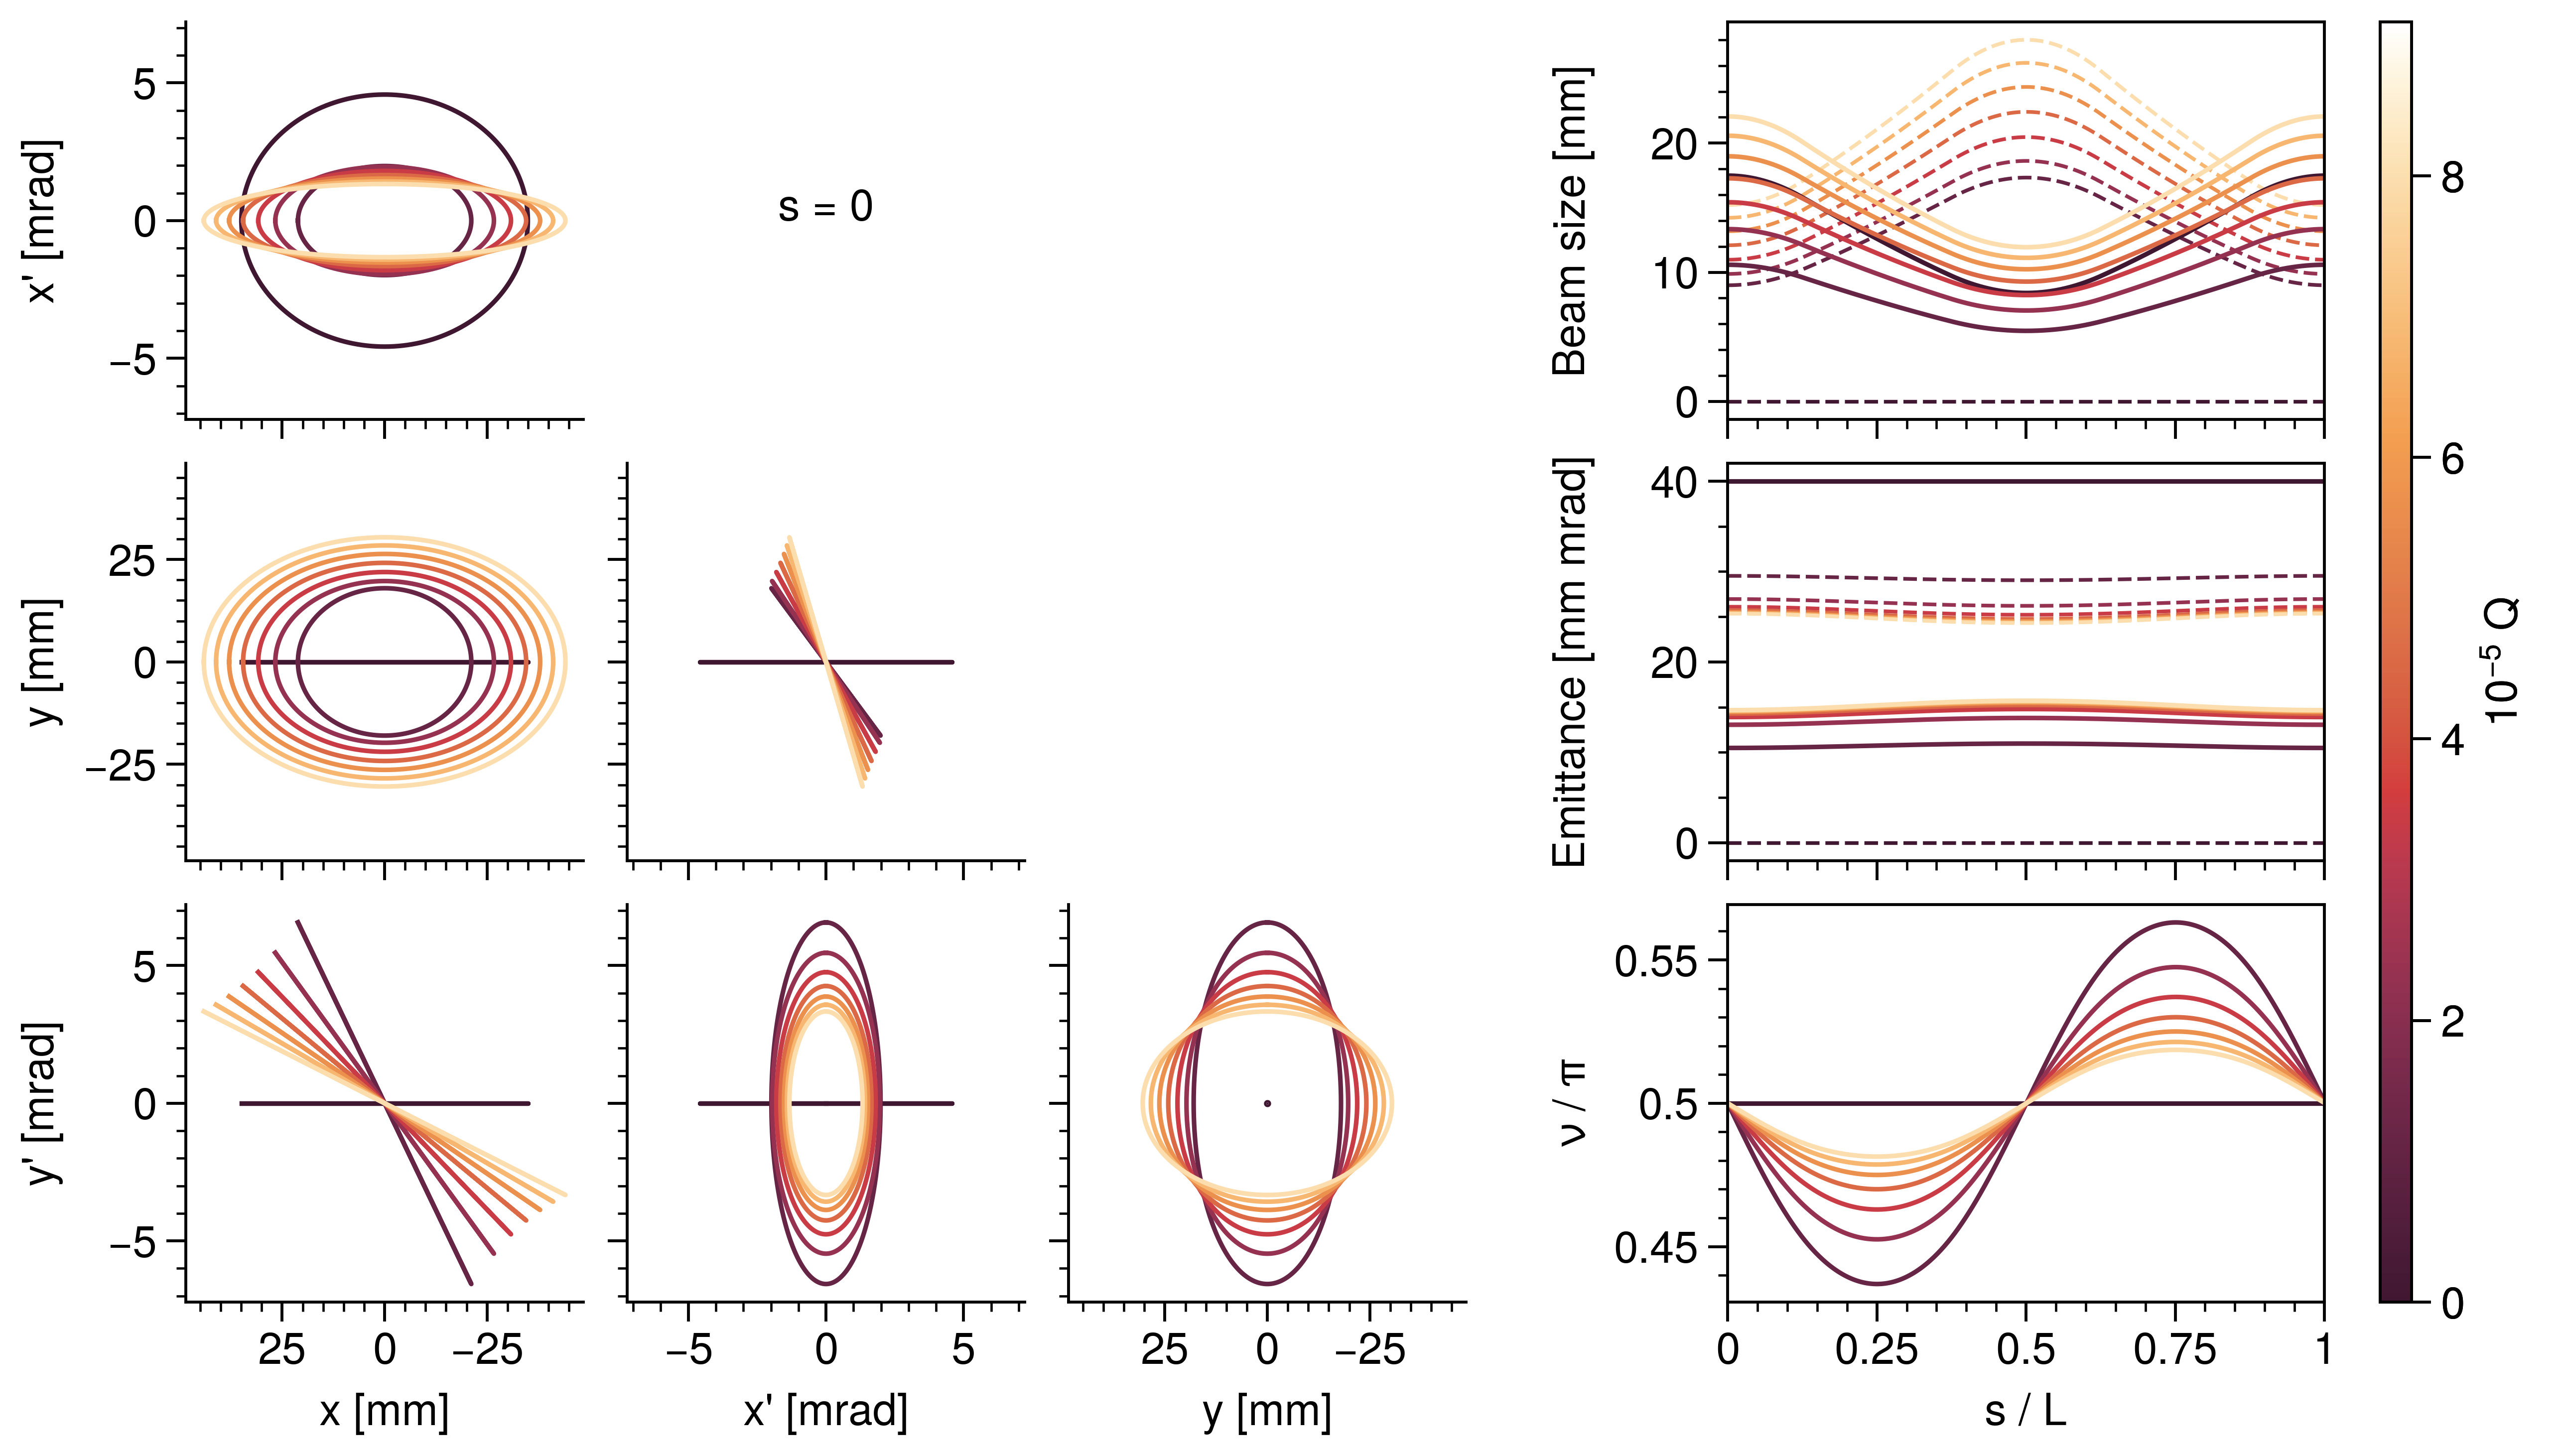
\includegraphics[width=\textwidth]{Images/chapter2/matched_vs_sc_fodo_split_mode1.png}
        \caption{Solution 1}
        \label{fig:matched_vs_sc_fodo_split_a}
    \end{subfigure}
    \vfill
    % \vspace*{1.0cm}
    \vfill
    \begin{subfigure}{1.0\textwidth}
        \centering
        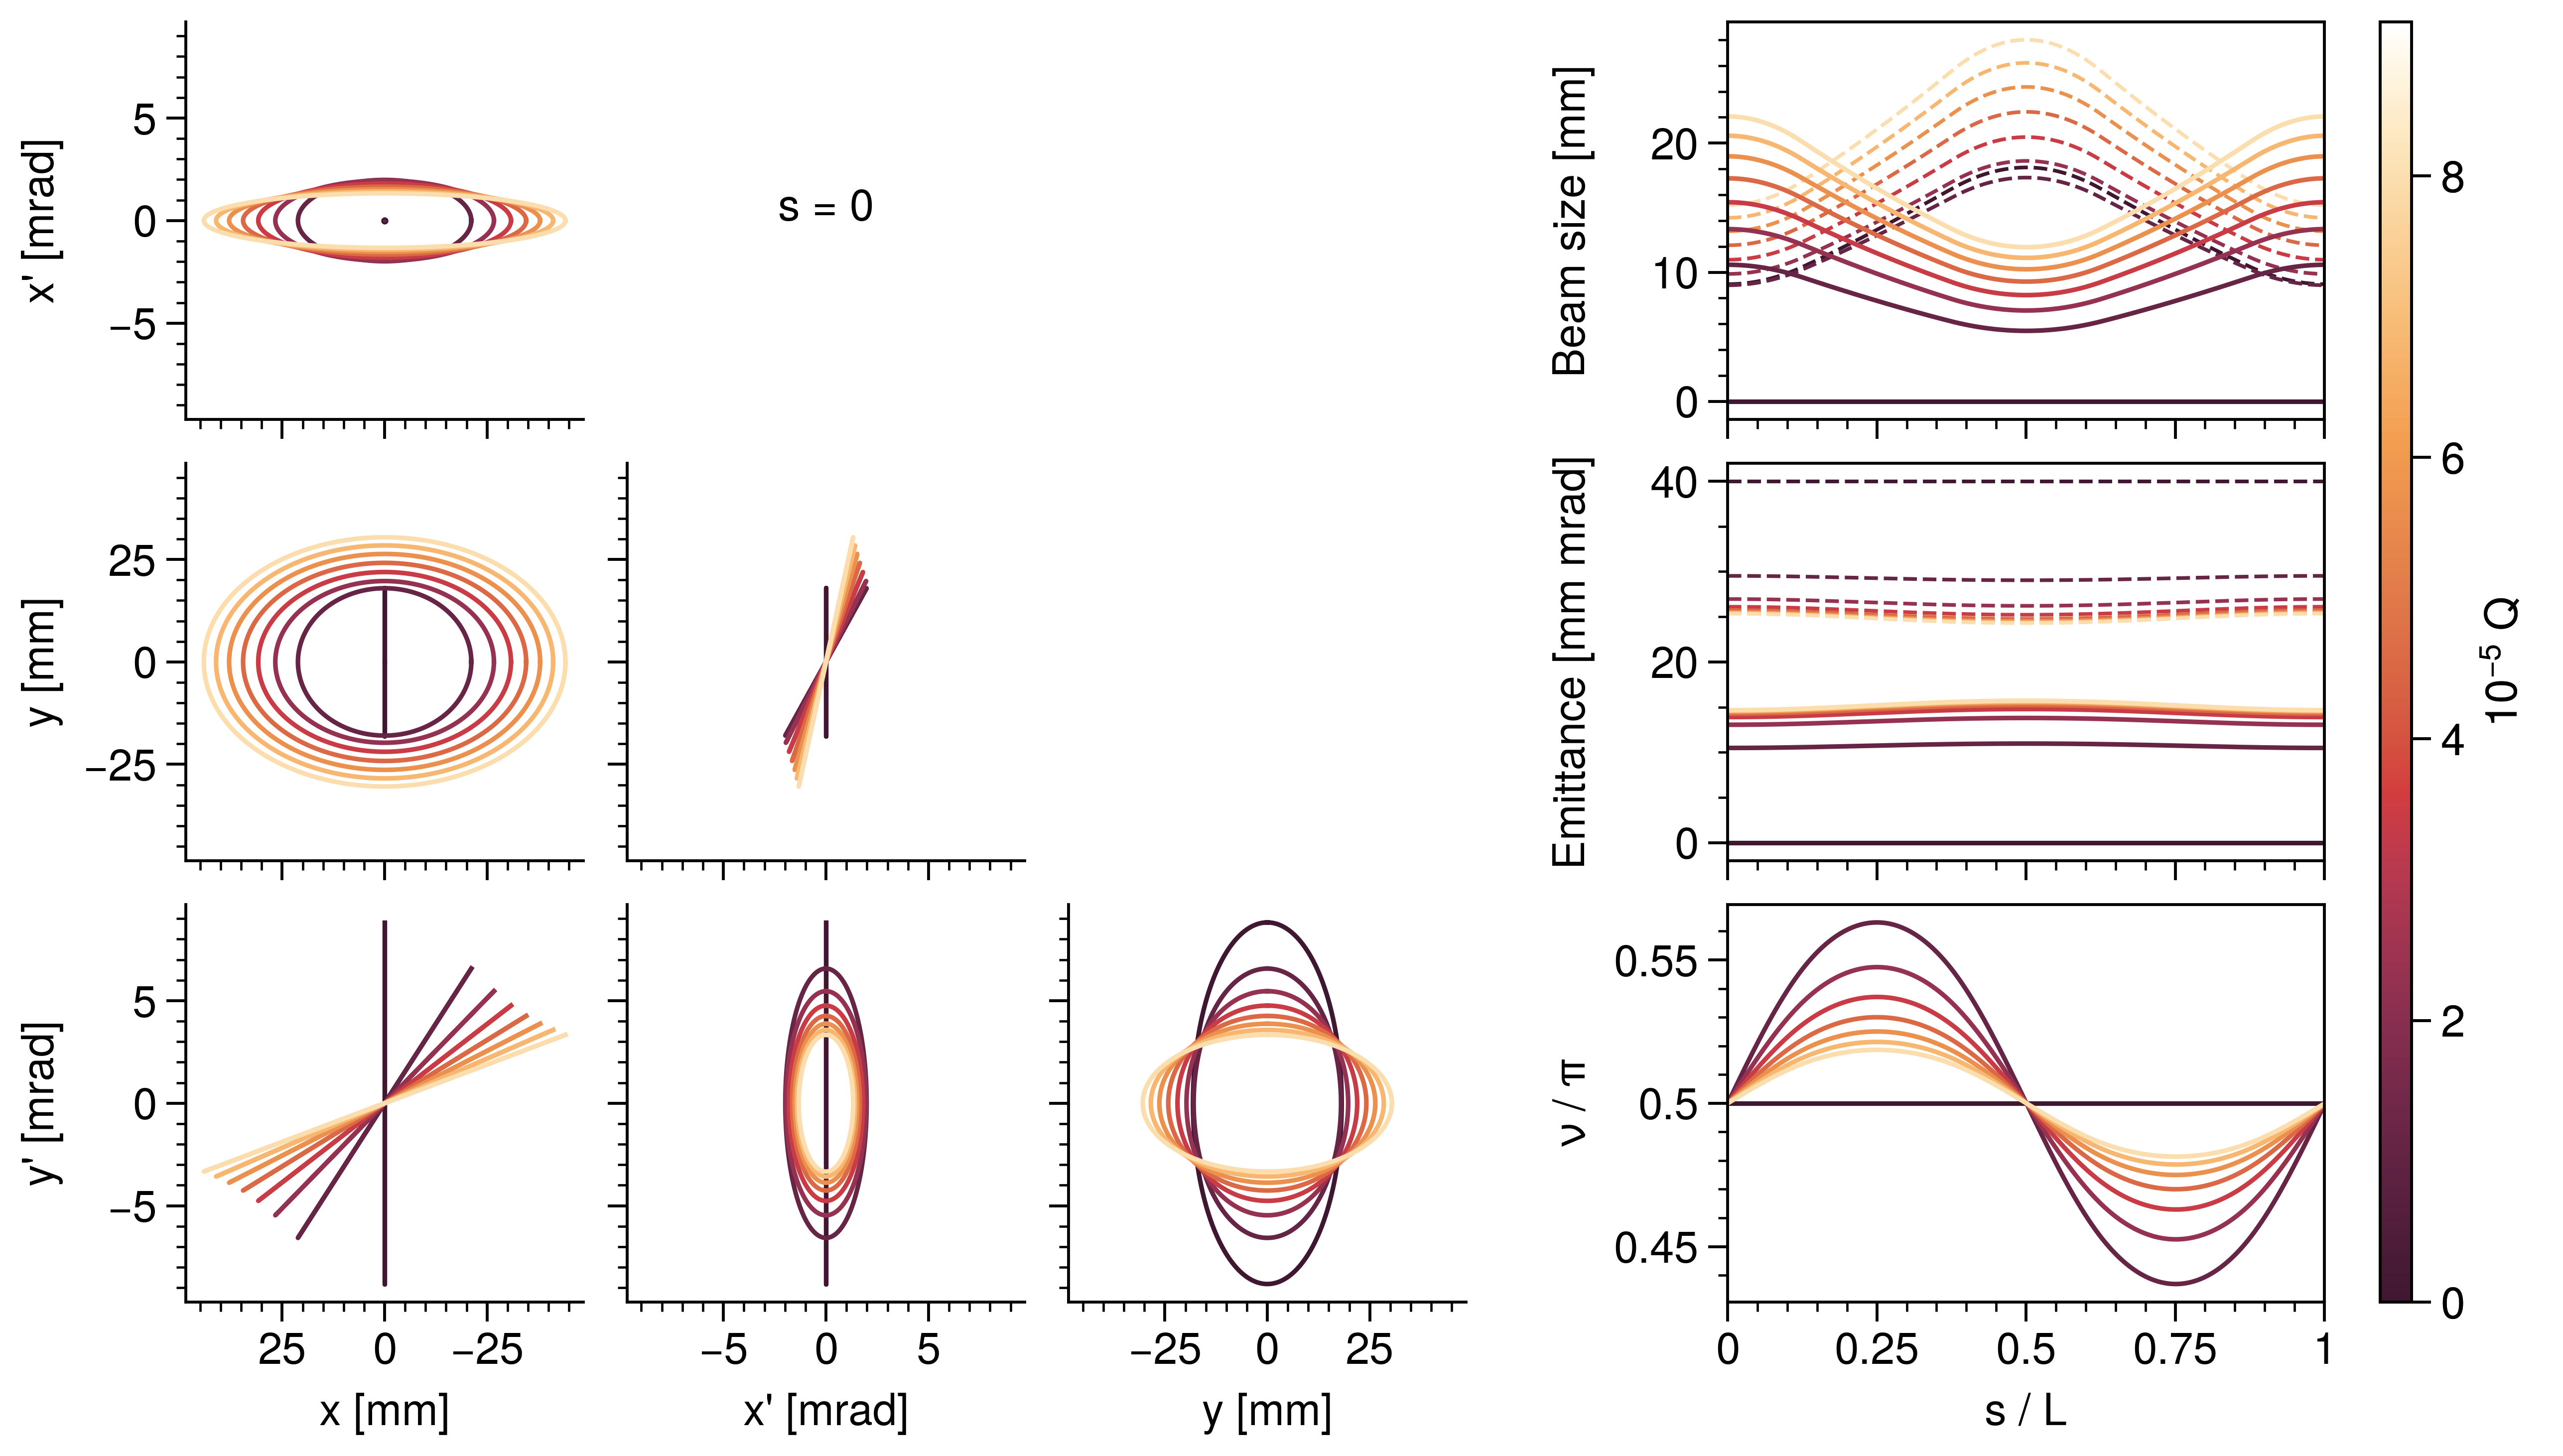
\includegraphics[width=\textwidth]{Images/chapter2/matched_vs_sc_fodo_split_mode2.png}
        \caption{Solution 2}
        \label{fig:matched_vs_sc_fodo_split_b}
    \end{subfigure}
    \caption{Matched envelope of the Danilov distribution in an uncoupled FODO lattice with unequal tunes as space charge is increased. Left: phase space projections at the lattice entrance. Right: beam parameters within the lattice. Solid lines are for $x$ and dashed lines are for $y$ in the top two plots.}
    \label{fig:matched_vs_sc_fodo_split}
\end{figure}
%
A notable feature of the zero space charge solutions is that they are flat. As noted in the discussion of elliptical painting in Section \ref{sec:Physically realizing a self-consistent distribution}, this is because the eigenvectors of the transfer matrix are uncoupled, meaning that $\mathbf{v}_1$ has no component in the $y-y'$ plane and $\mathbf{v}_2$ has no component in the $x-x'$ plane. The intrinsic and apparent emittances of the matched beam therefore coincide. (Note that $\nu$ is undefined in this case, but we chose to draw a flat line at $\nu = 90\degree$.) In Fig.~\ref{fig:matched_vs_sc_fodo_split}, since the lattice tunes are equal, any linear combination of eigenvectors is itself an eigenvector; the matched beam can be round, flat, or anything in-between. 

The beam dynamics with space charge are very similar to the previous case of equal tunes, and the two solutions are again related by opposite signs of their angular momentum. The most notable effect of space charge on the matched beam is to significantly split the apparent emittances. This is expected since space charge now needs to decrease the horizontal and vertical tunes by different amounts such that they are equal in the end. When space charge is weak, the emittances are maximally split; as space charge is increased, the emittances move closer together. We also note that the horizontal emittance in both solutions is always greater than the vertical emittance when space charge is turned on; This follows from the fact that the zero-current tune is larger in the horizontal plane than in the vertical plane, so space charge must provide more defocusing in the vertical plane.






\subsubsection{Coupled lattice}

The same information as in Fig.~\ref{fig:matched_vs_sc_fodo} and Fig.~\ref{fig:matched_vs_sc_fodo_split} is plotted in Fig.~\ref{fig:matched_vs_sc_fodo_skew} for the skew quadrupole lattice in Fig.~\ref{fig:fodo_lattices}b.
%
\begin{figure}[!p]
    \begin{subfigure}{1.0\textwidth}
        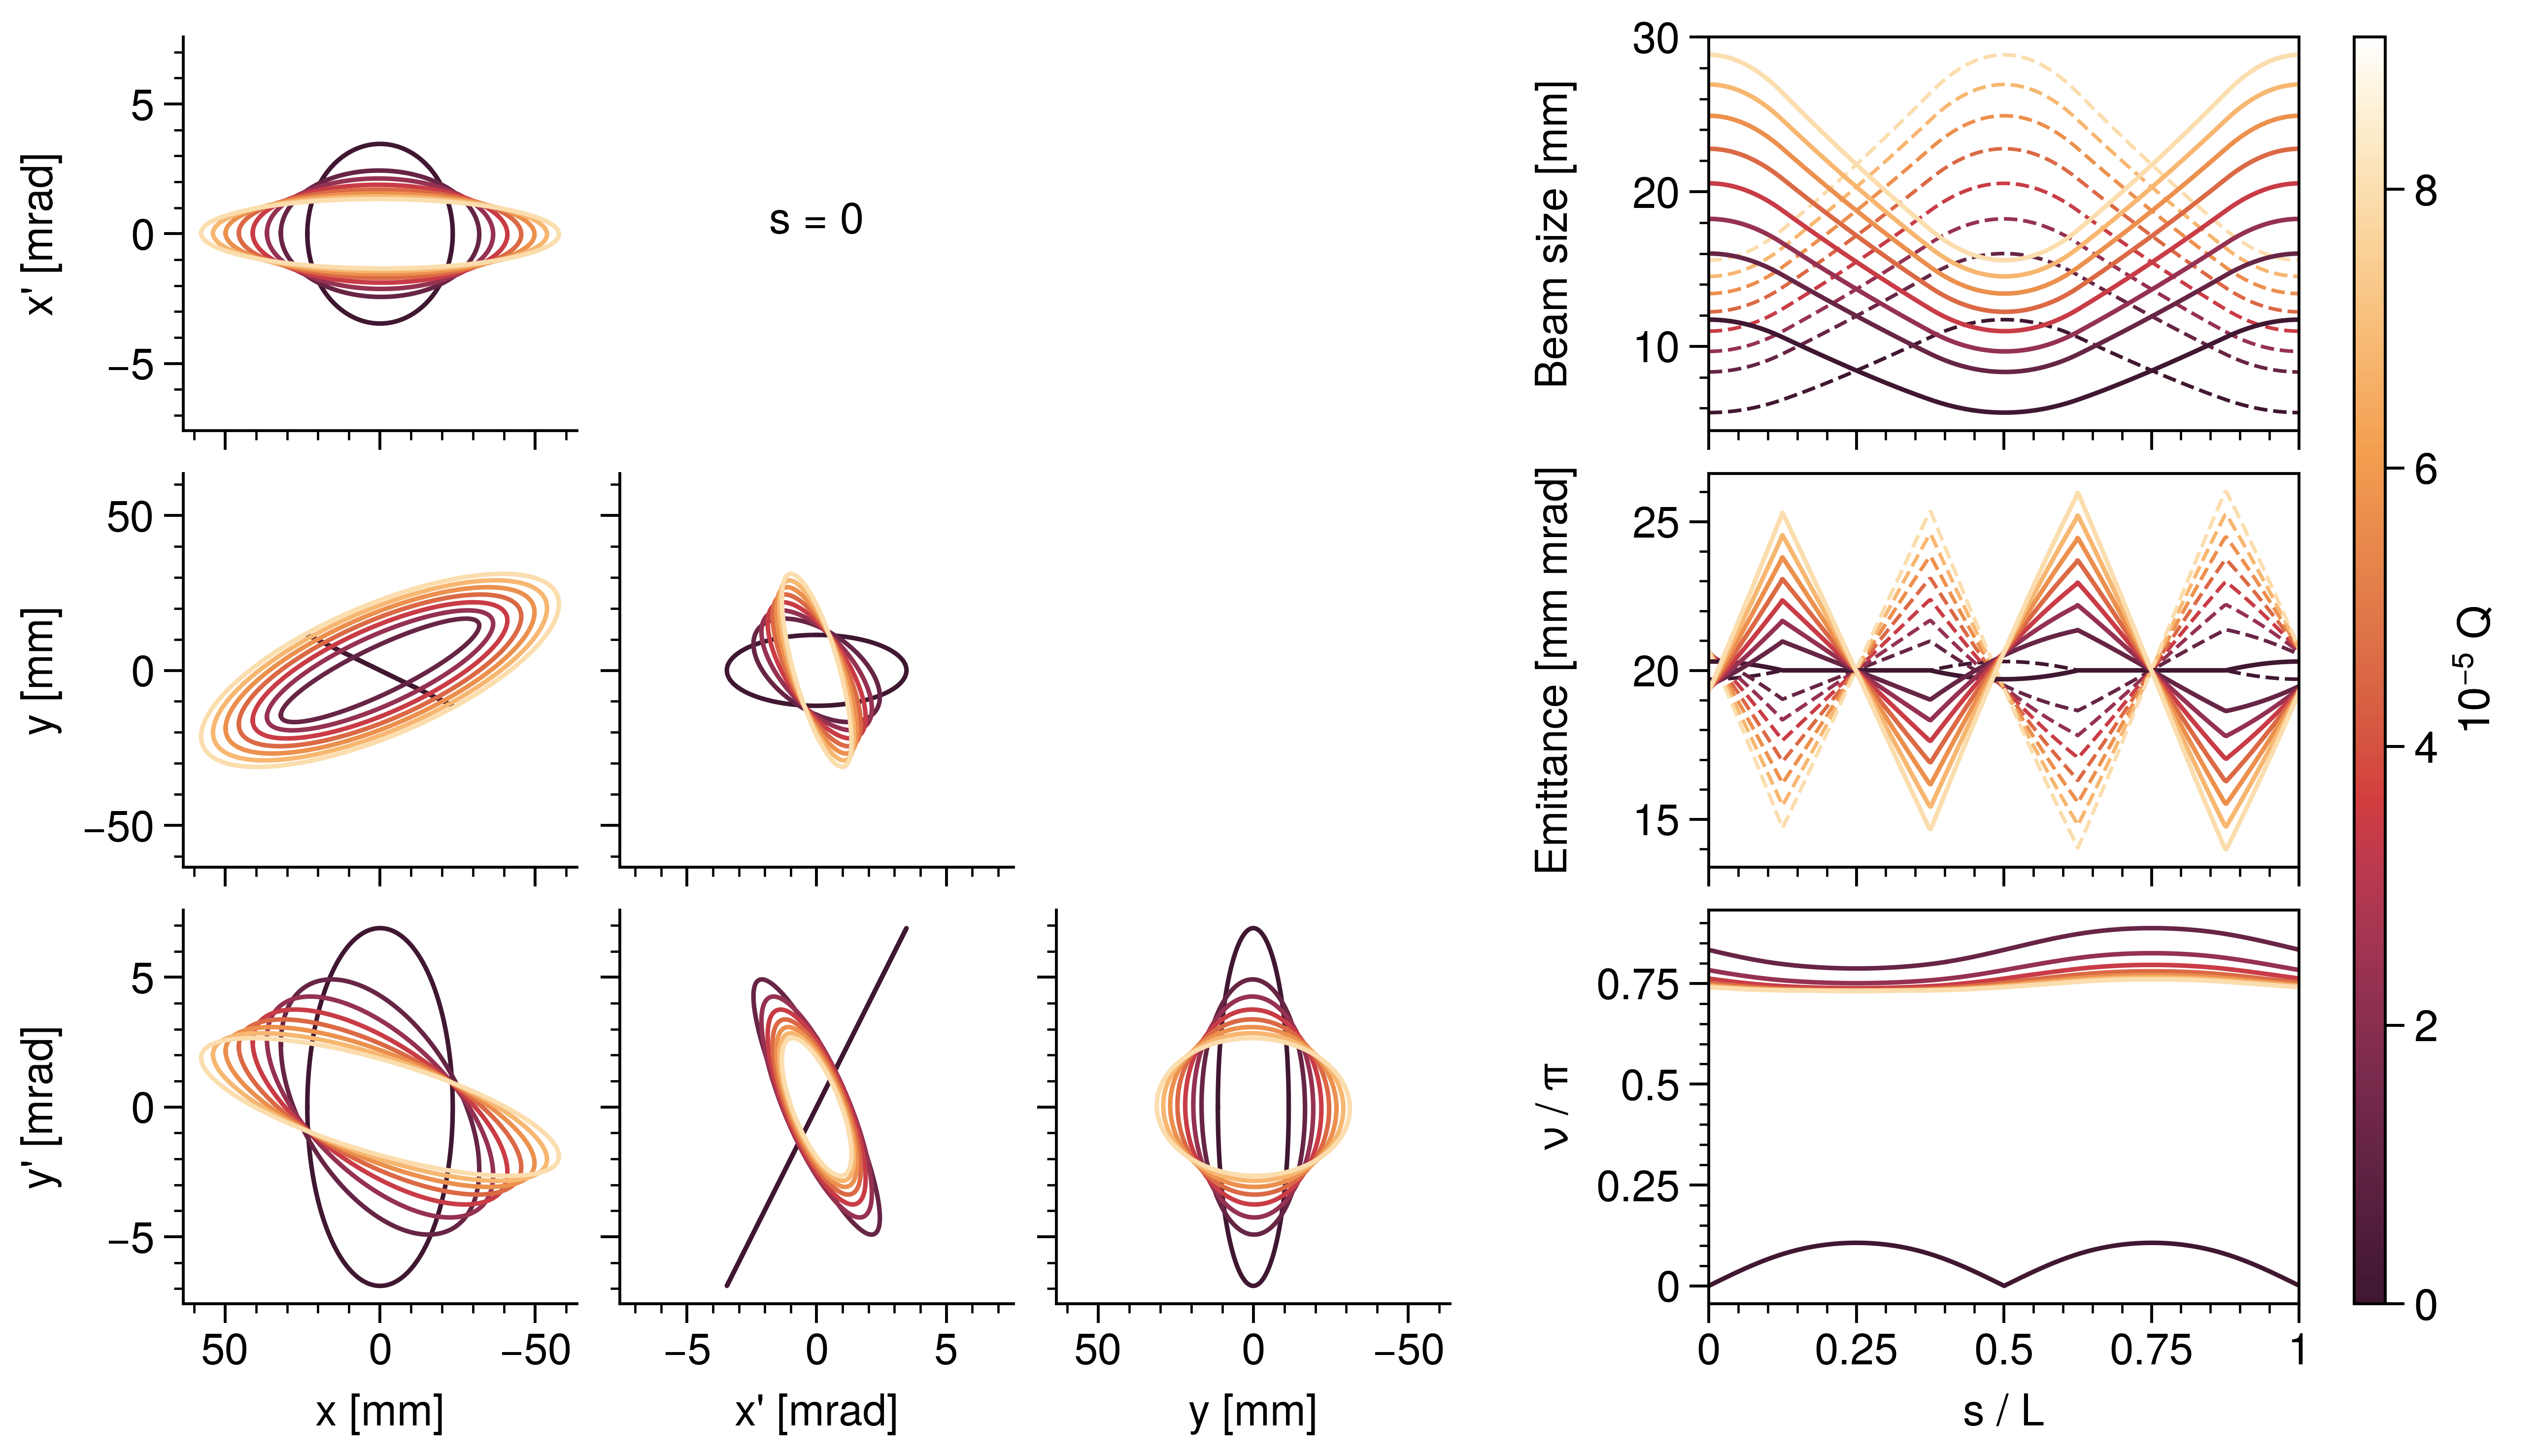
\includegraphics[width=\textwidth]{Images/chapter2/matched_vs_sc_fodo_skew_mode1.png}
        \caption{Solution 1}
        \label{fig:matched_vs_sc_fodo_skew_a}
    \end{subfigure}
    \vfill
    % \vspace*{1.0cm}
    \vfill
    \begin{subfigure}{1.0\textwidth}
        \centering
        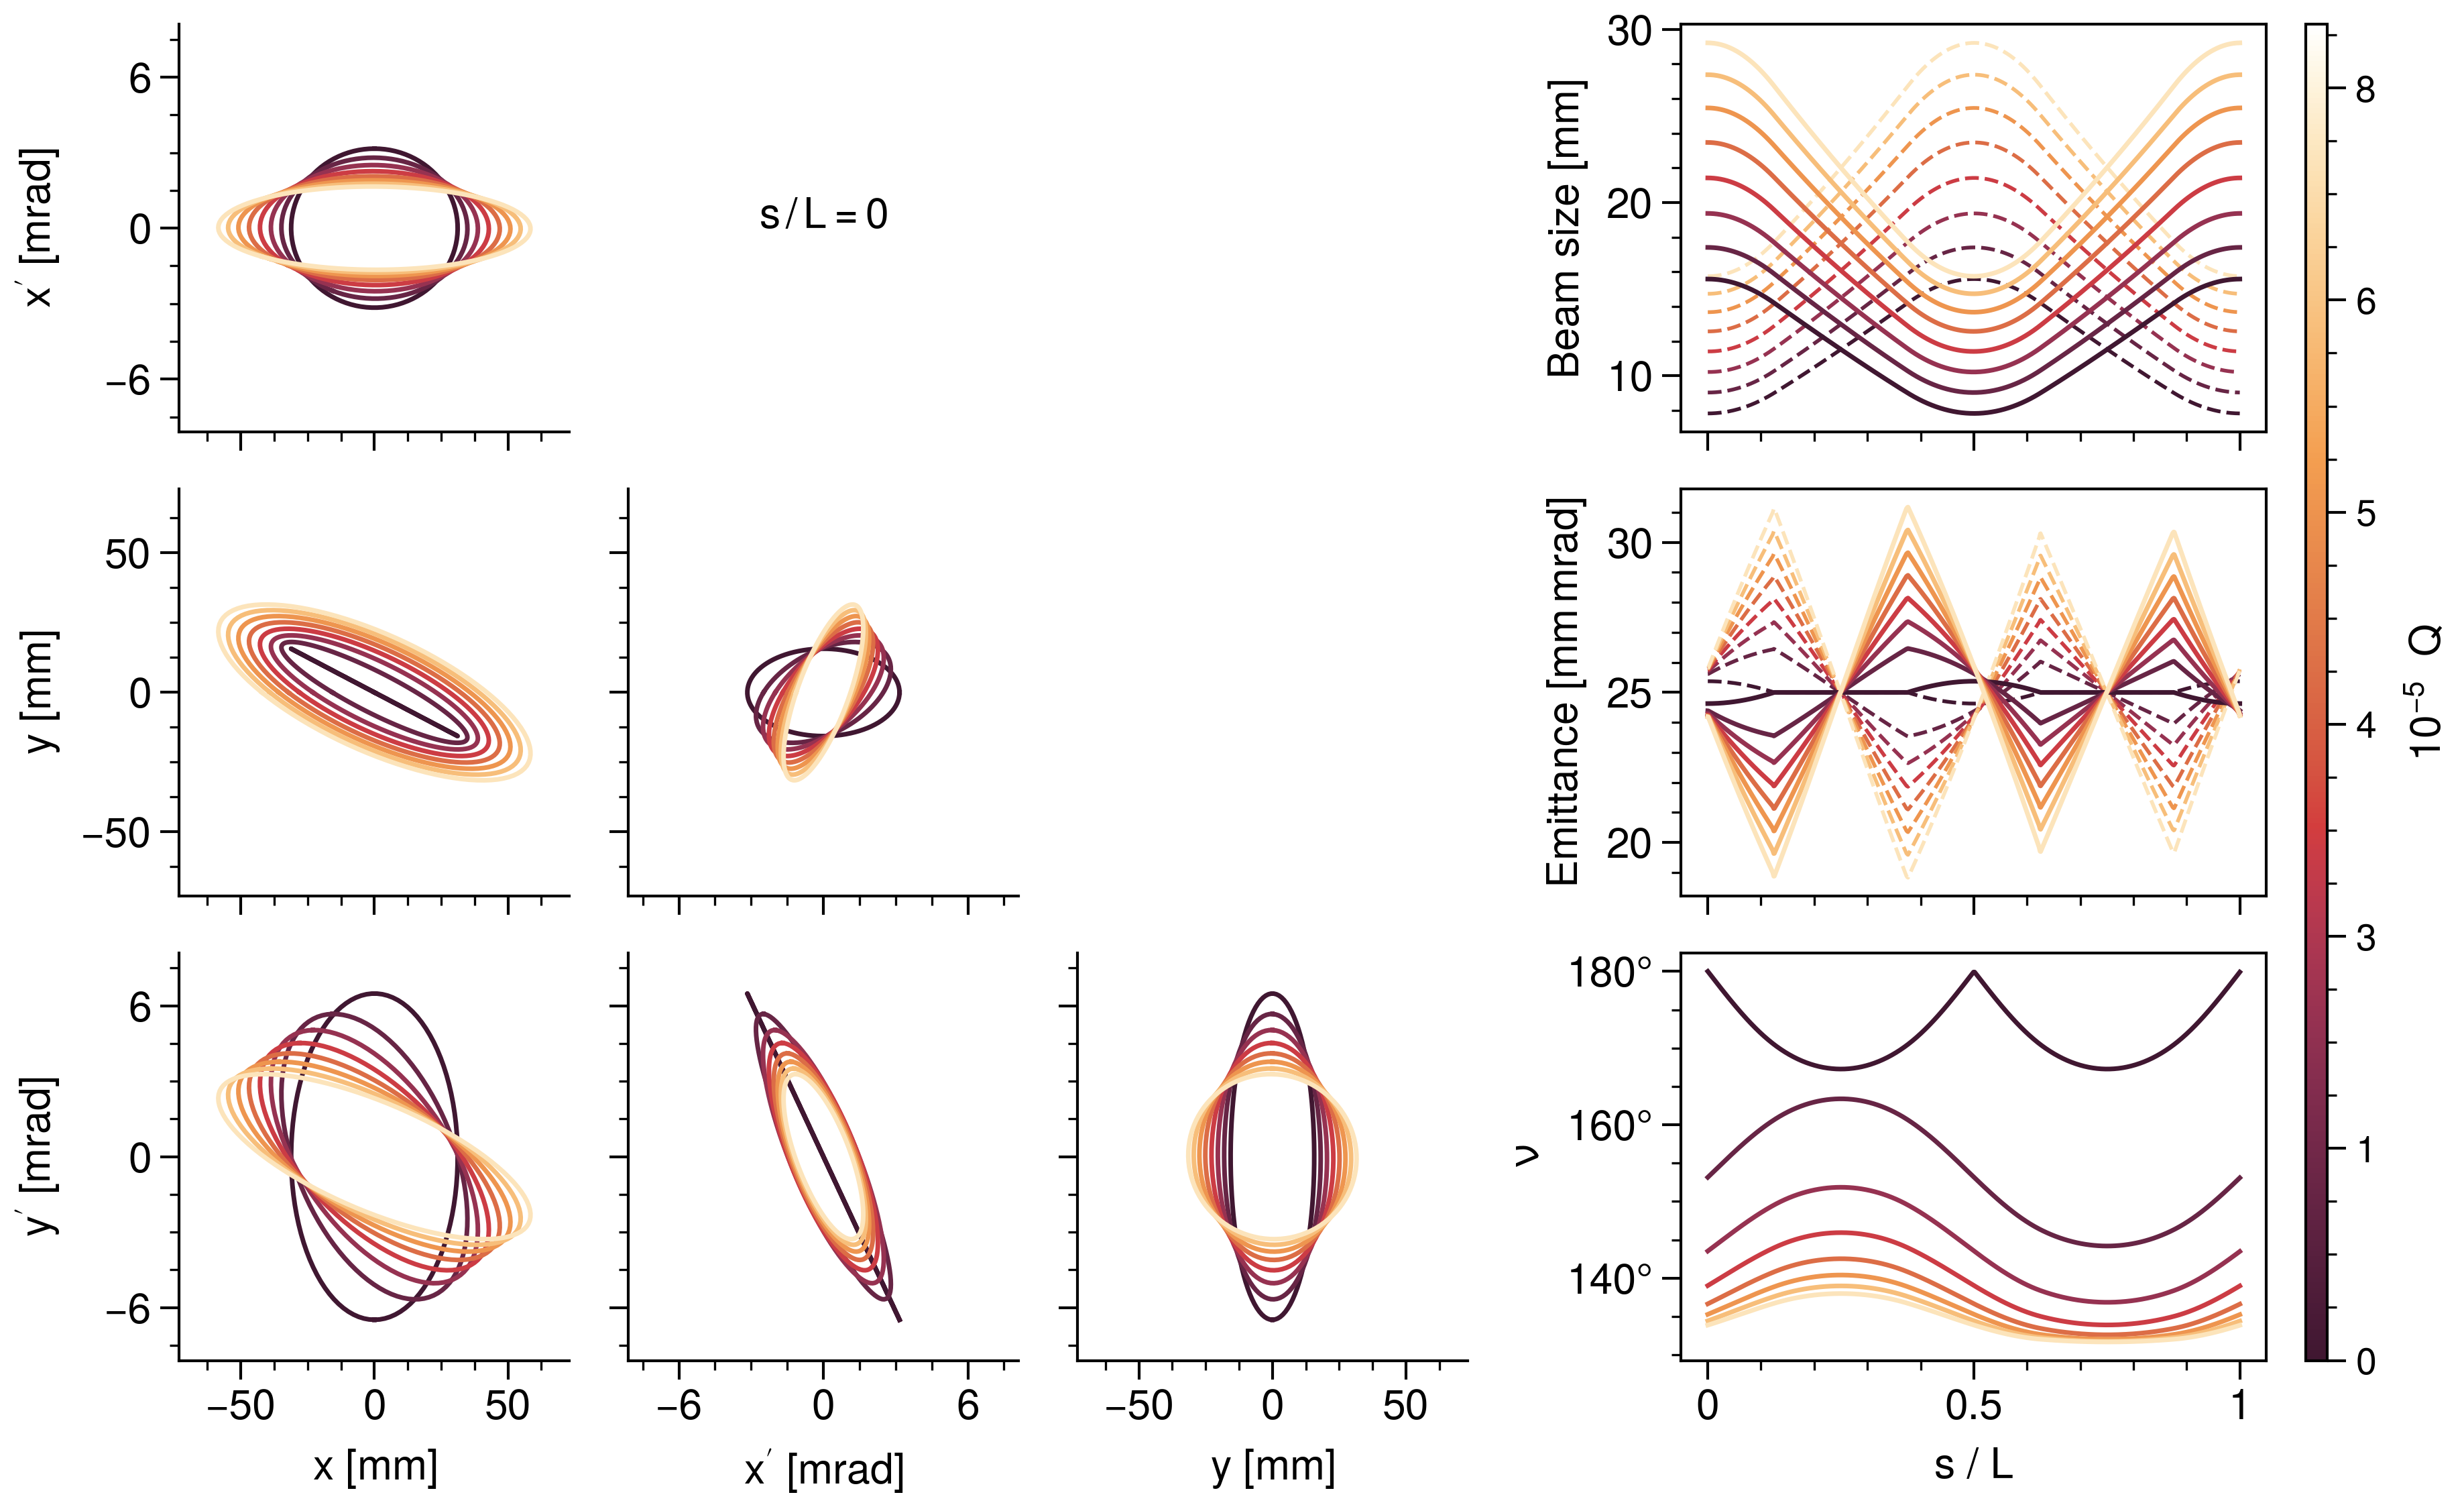
\includegraphics[width=\textwidth]{Images/chapter2/matched_vs_sc_fodo_skew_mode2.png}
        \caption{Solution 2}
        \label{fig:matched_vs_sc_fodo_skew_b}
    \end{subfigure}
    \caption{Matched envelope of the Danilov distribution in a coupled FODO lattice as space  charge is increased. The lattice is coupled due to skew quadrupoles. Left: phase space projections at the lattice entrance. Right: beam parameters within the lattice. Solid lines are for $x$ and dashed lines are for $y$ in the top two plots.}
    \label{fig:matched_vs_sc_fodo_skew}
\end{figure}
%
The locations of the skew quadrupoles are evident from the small arcs in the emittance curves. Without space charge, the matched beam at the center of the quadrupoles projects to a diagonal line in real space ($\nu = 0\degree$ or $180\degree$) with zero angular momentum, and the two solutions differ in the sign of the tilt angle of this line. The addition of space charge pulls $\nu$ away from these extreme values, resulting in a nonzero beam area. The cross-plane correlations between the positions and slopes also become nonzero as a consequence, again revealing the opposite directions of the angular momentum between the two solutions. 

An interesting property of the matched beams is the asymmetry between the two solutions. The presence of space charge leads to two solutions with the same tilt angle in the $x$-$y$ plane, as opposed to opposite tilt angles without space charge. This abrupt change in the matched beam orientation in solution 1 causes the optimizer to struggle for low space charge, often terminating due to a lack of progress. Fig.~\ref{fig:optimizer_comparison_a} shows the final cost as a function of the beam perveance, and Fig.~\ref{fig:optimizer_comparison_b} shows the turn-by-turn oscillations of the $\nu$ parameter for a subset of these cases. 
%
\begin{figure}[!p]
    \centering
    \begin{subfigure}{0.8\textwidth}
        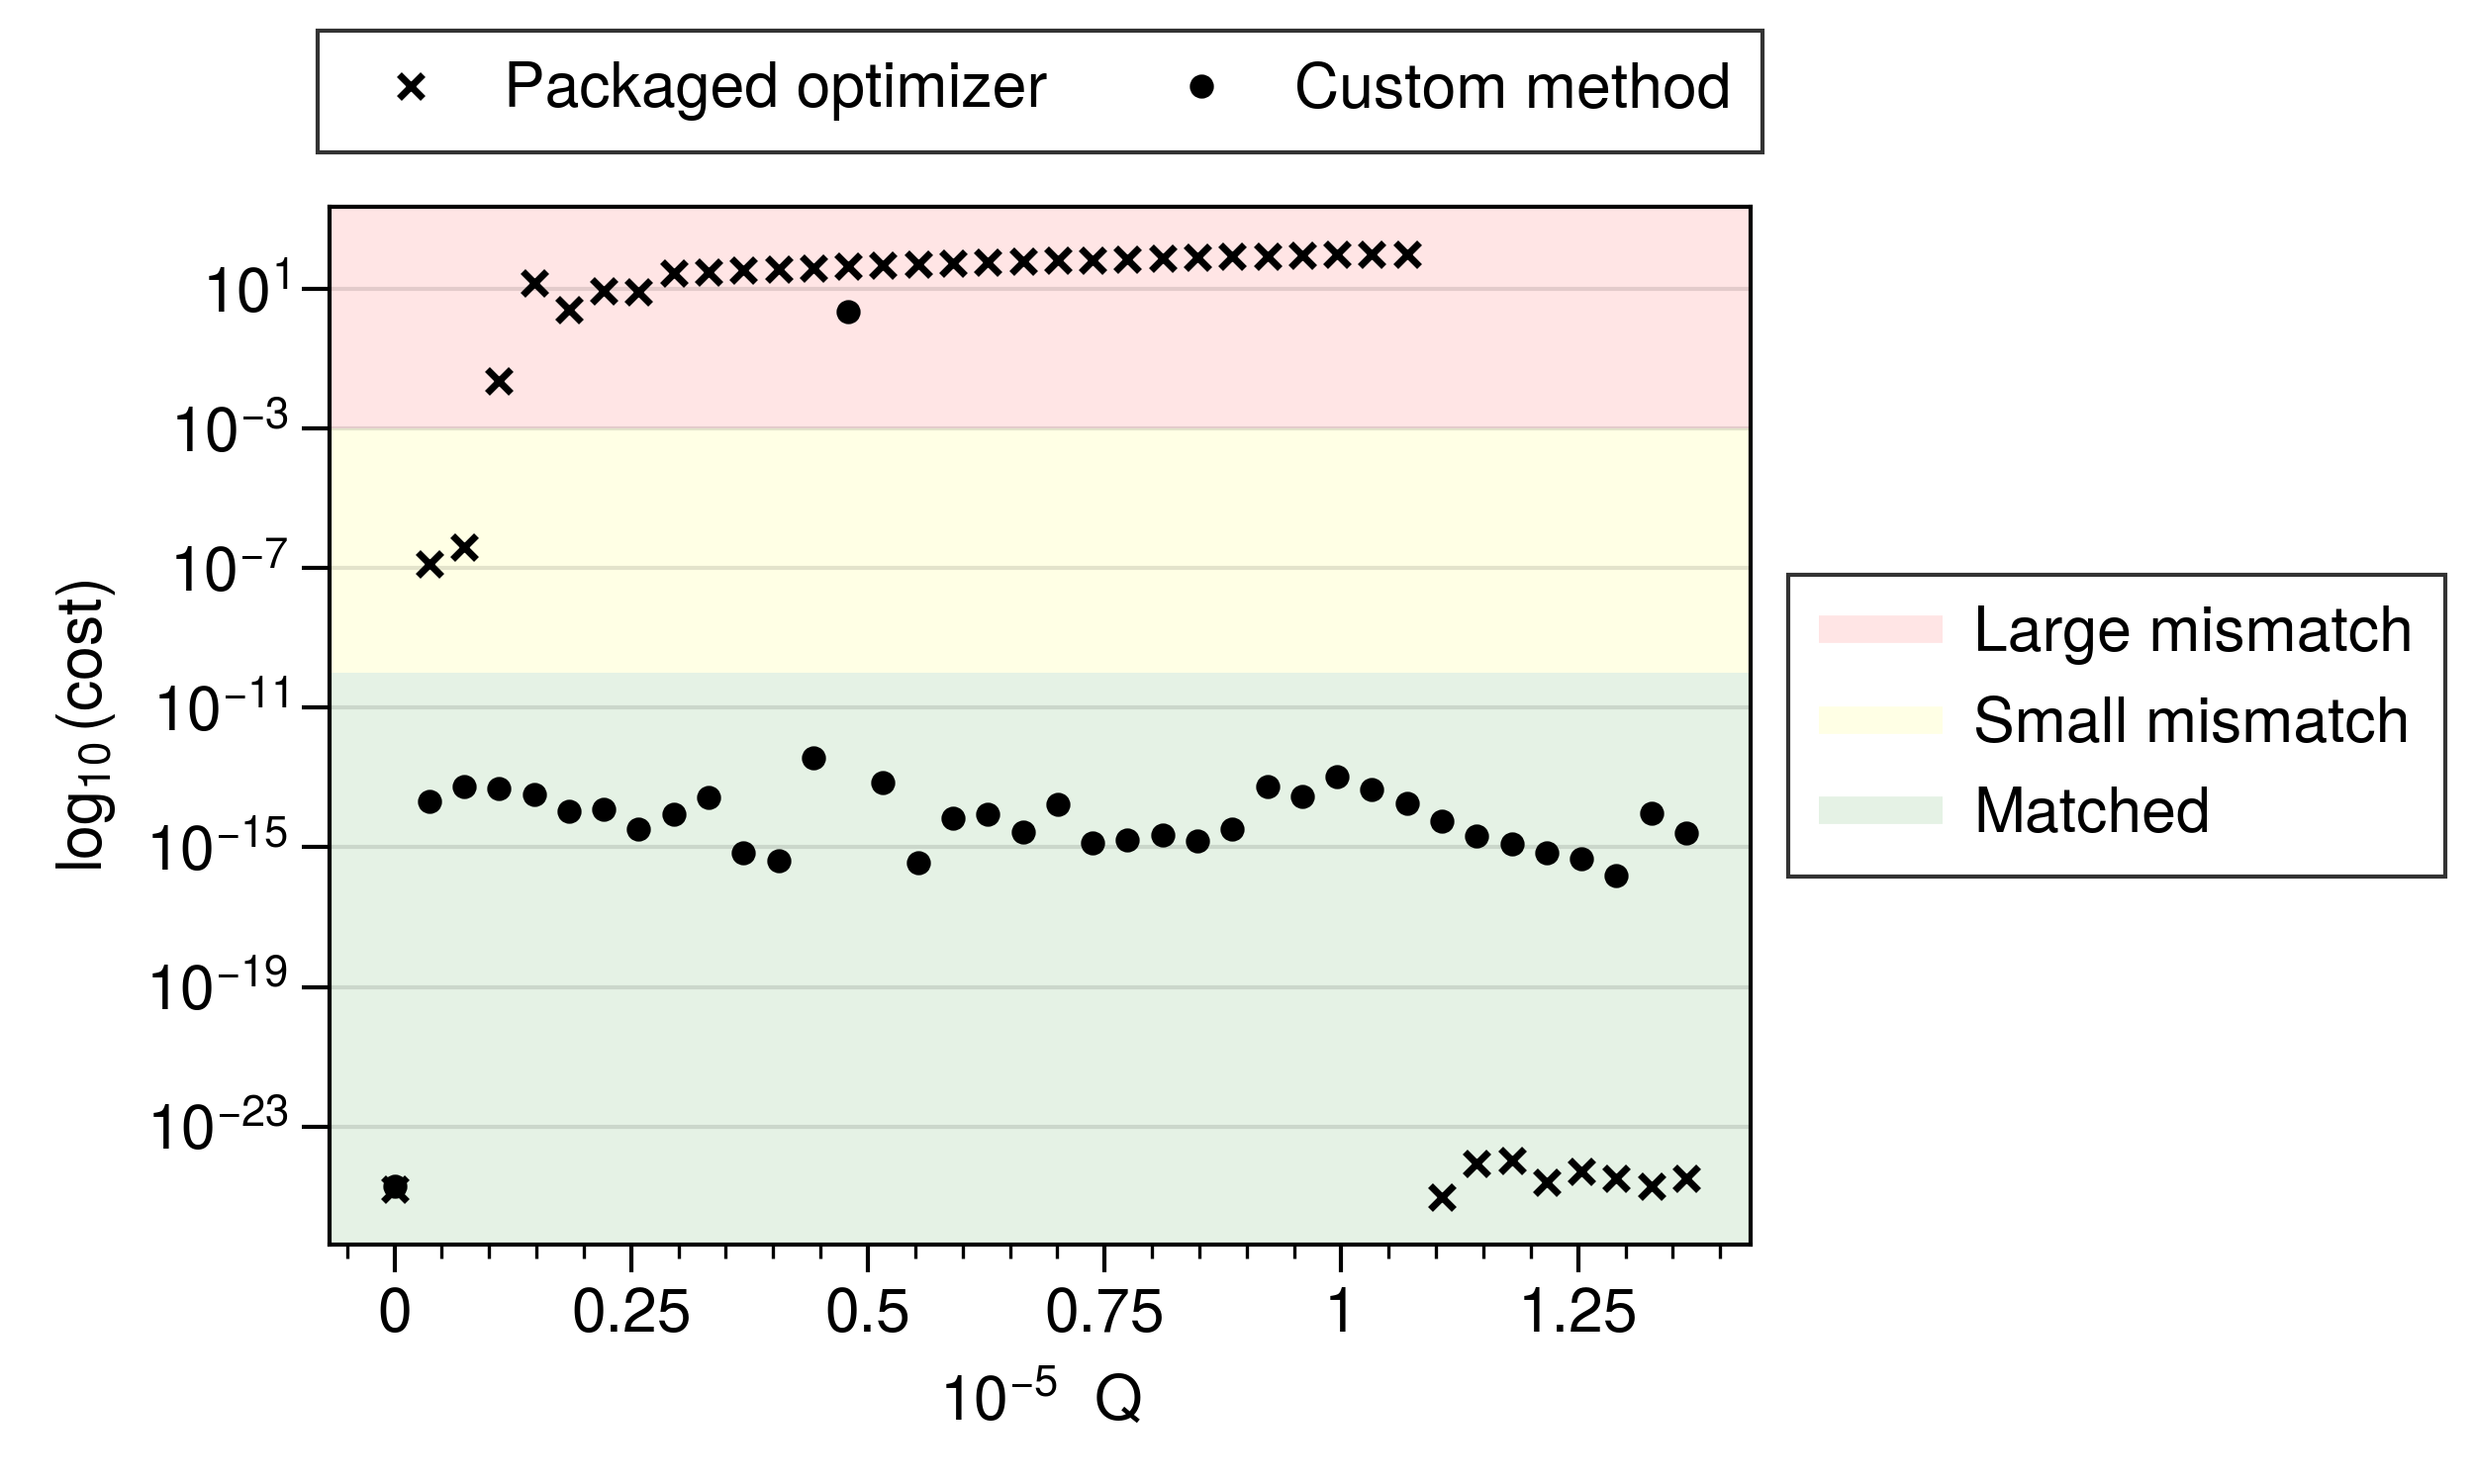
\includegraphics[width=\textwidth]{Images/chapter2/optimizer_comparison_costfunc.png}
        \caption{}
        \label{fig:optimizer_comparison_a}
    \end{subfigure}
    \vfill
    \vspace*{1cm}
    \vfill
    \begin{subfigure}{1.0\textwidth}
        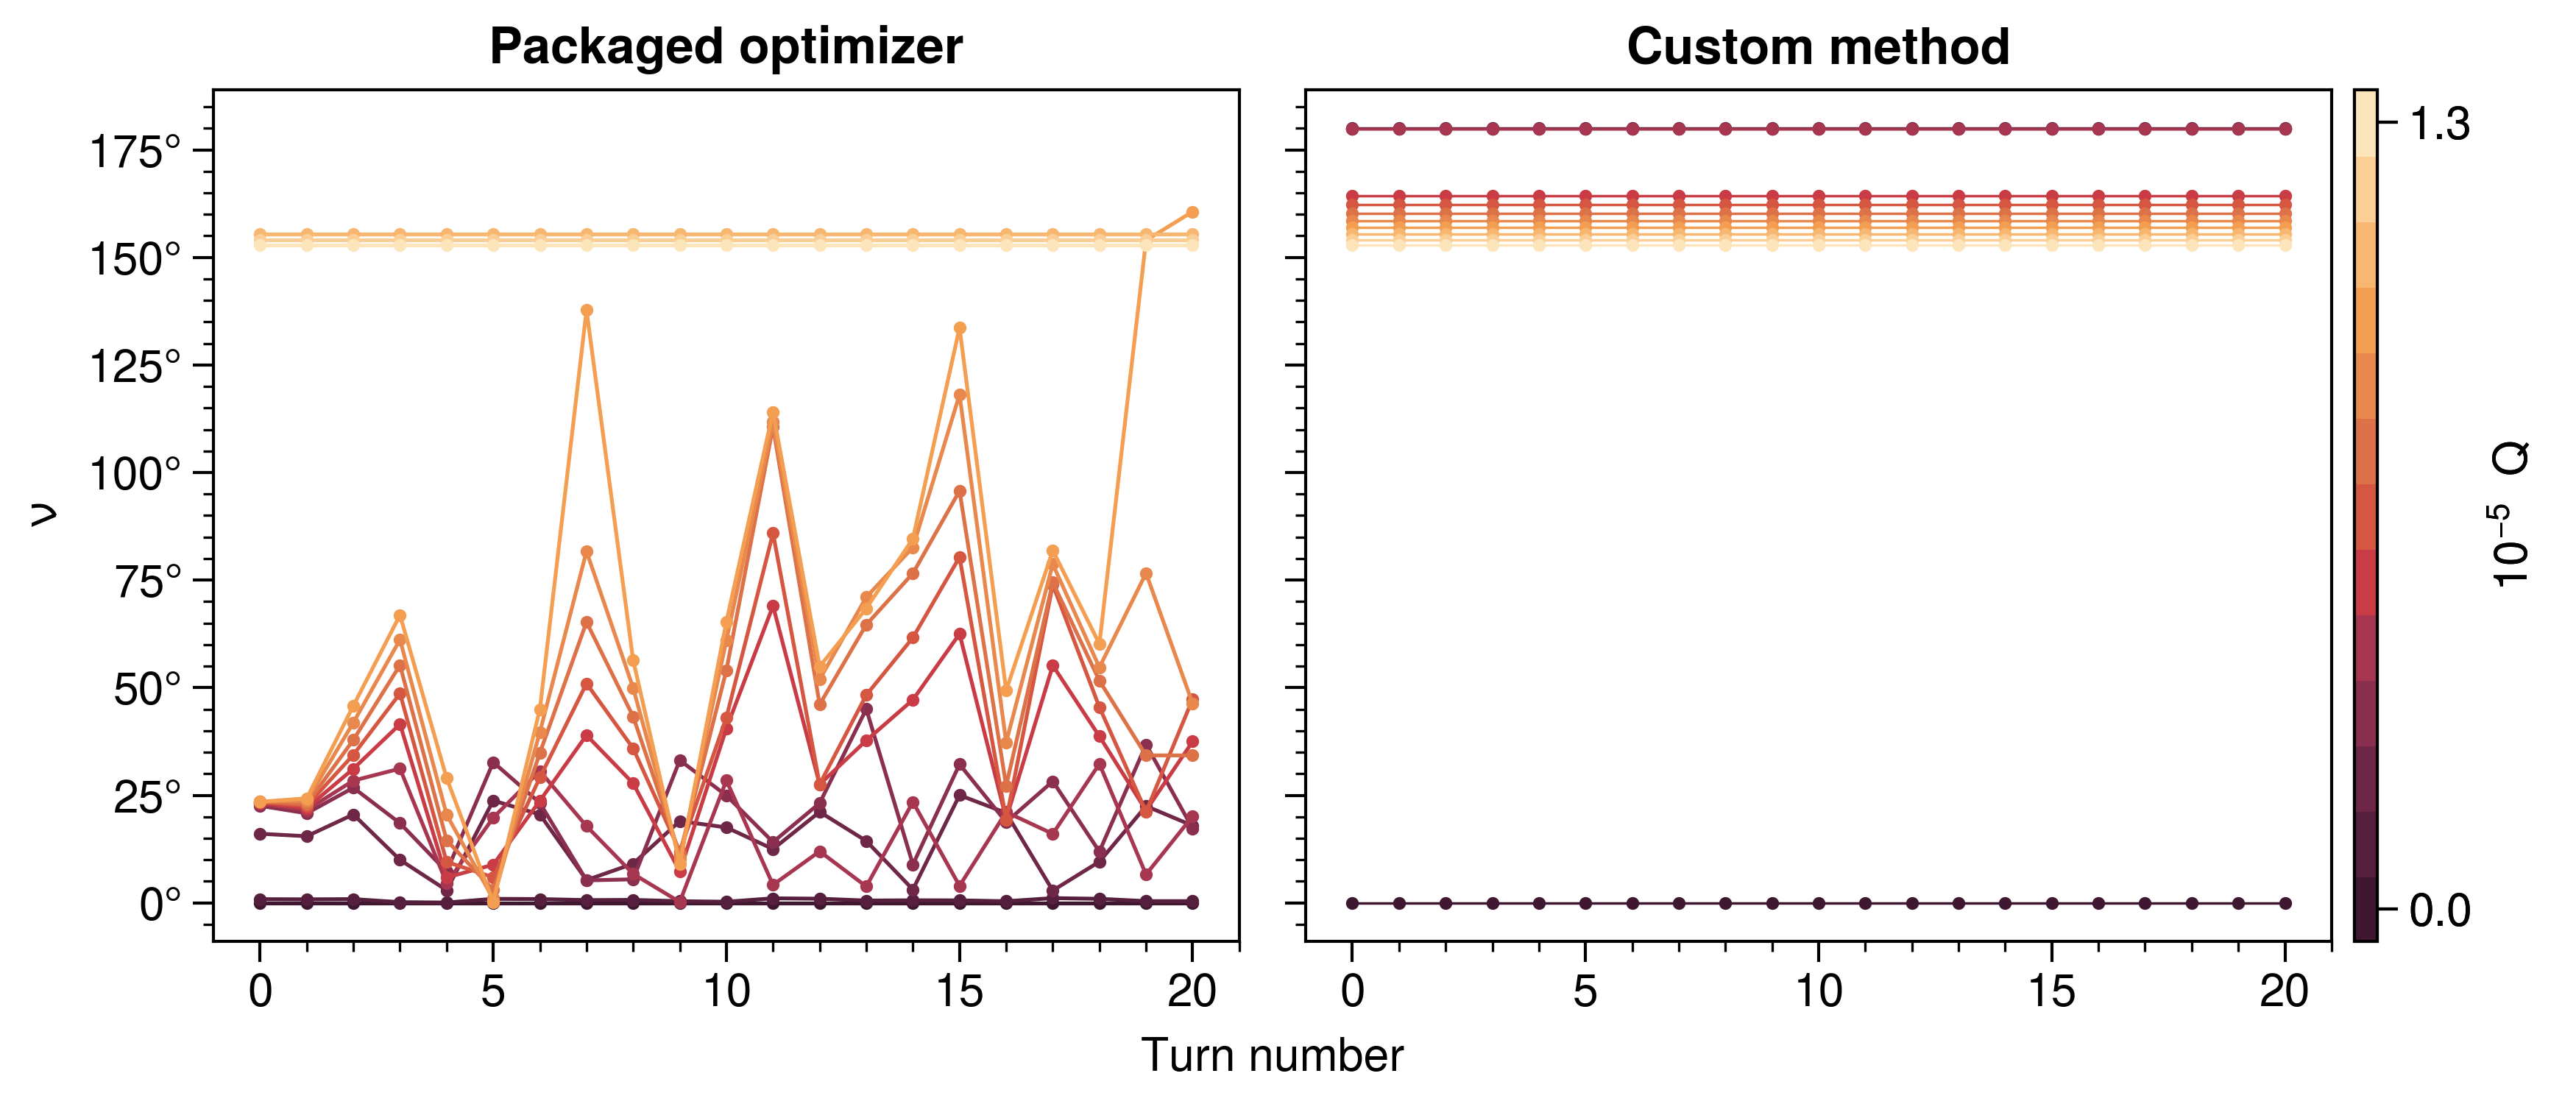
\includegraphics[width=\textwidth]{Images/chapter2/optimizer_comparison_tbt.png}
        \caption{}
        \label{fig:optimizer_comparison_b}
    \end{subfigure}
    \caption{Performance of the matching algorithm in a skew quadrupole lattice, corresponding to solution 1 in Fig.~\ref{fig:matched_vs_sc_fodo_skew_a}. (a) Final value of the cost function as a function of the beam perveance. (b) Turn-by-turn oscillations of the $\nu$ parameter after running each algorithm.}
    \label{fig:optimizer_comparison}
\end{figure}
%
The matching routine is not run when $Q = 0$ since the beam is already matched to the bare lattice; this corresponds to the bottom line in both panels of Fig.~\ref{fig:optimizer_comparison_b} at $\nu = 0$. The final cost is therefore the same for the two algorithms at this point. For small but nonzero perveance, the optimizer converges to a beam with $\nu \approx 0$ which exhibits very small mismatch oscillations (yellow region). The oscillations become more severe as the perveance is increased (red region), which corresponds to lines starting at $\nu \approx 25\degree$ in Fig.~\ref{fig:optimizer_comparison_b}. An exact match is eventually found (green region) when the perveance is sufficiently large with $\nu \approx 150\degree$. The averaging method, on the other hand, finds the exact match in nearly all cases. (Note that the circles and crosses on the far right of Fig.~\ref{fig:optimizer_comparison_b} represent the same beam; the algorithms have just terminated at different final costs.) This discussion simply illustrates that some care must be taken for certain values of the beam perveance when skew quadrupoles are present.

As a final demonstration of the method, coupling was included by the insertion of solenoid magnets in Fig.~\ref{fig:fodo_lattices}c. The results are shown in Fig.~\ref{fig:matched_vs_sc_fodo_sol}.
%
\begin{figure}[!p]
    \begin{subfigure}{1.0\textwidth}
        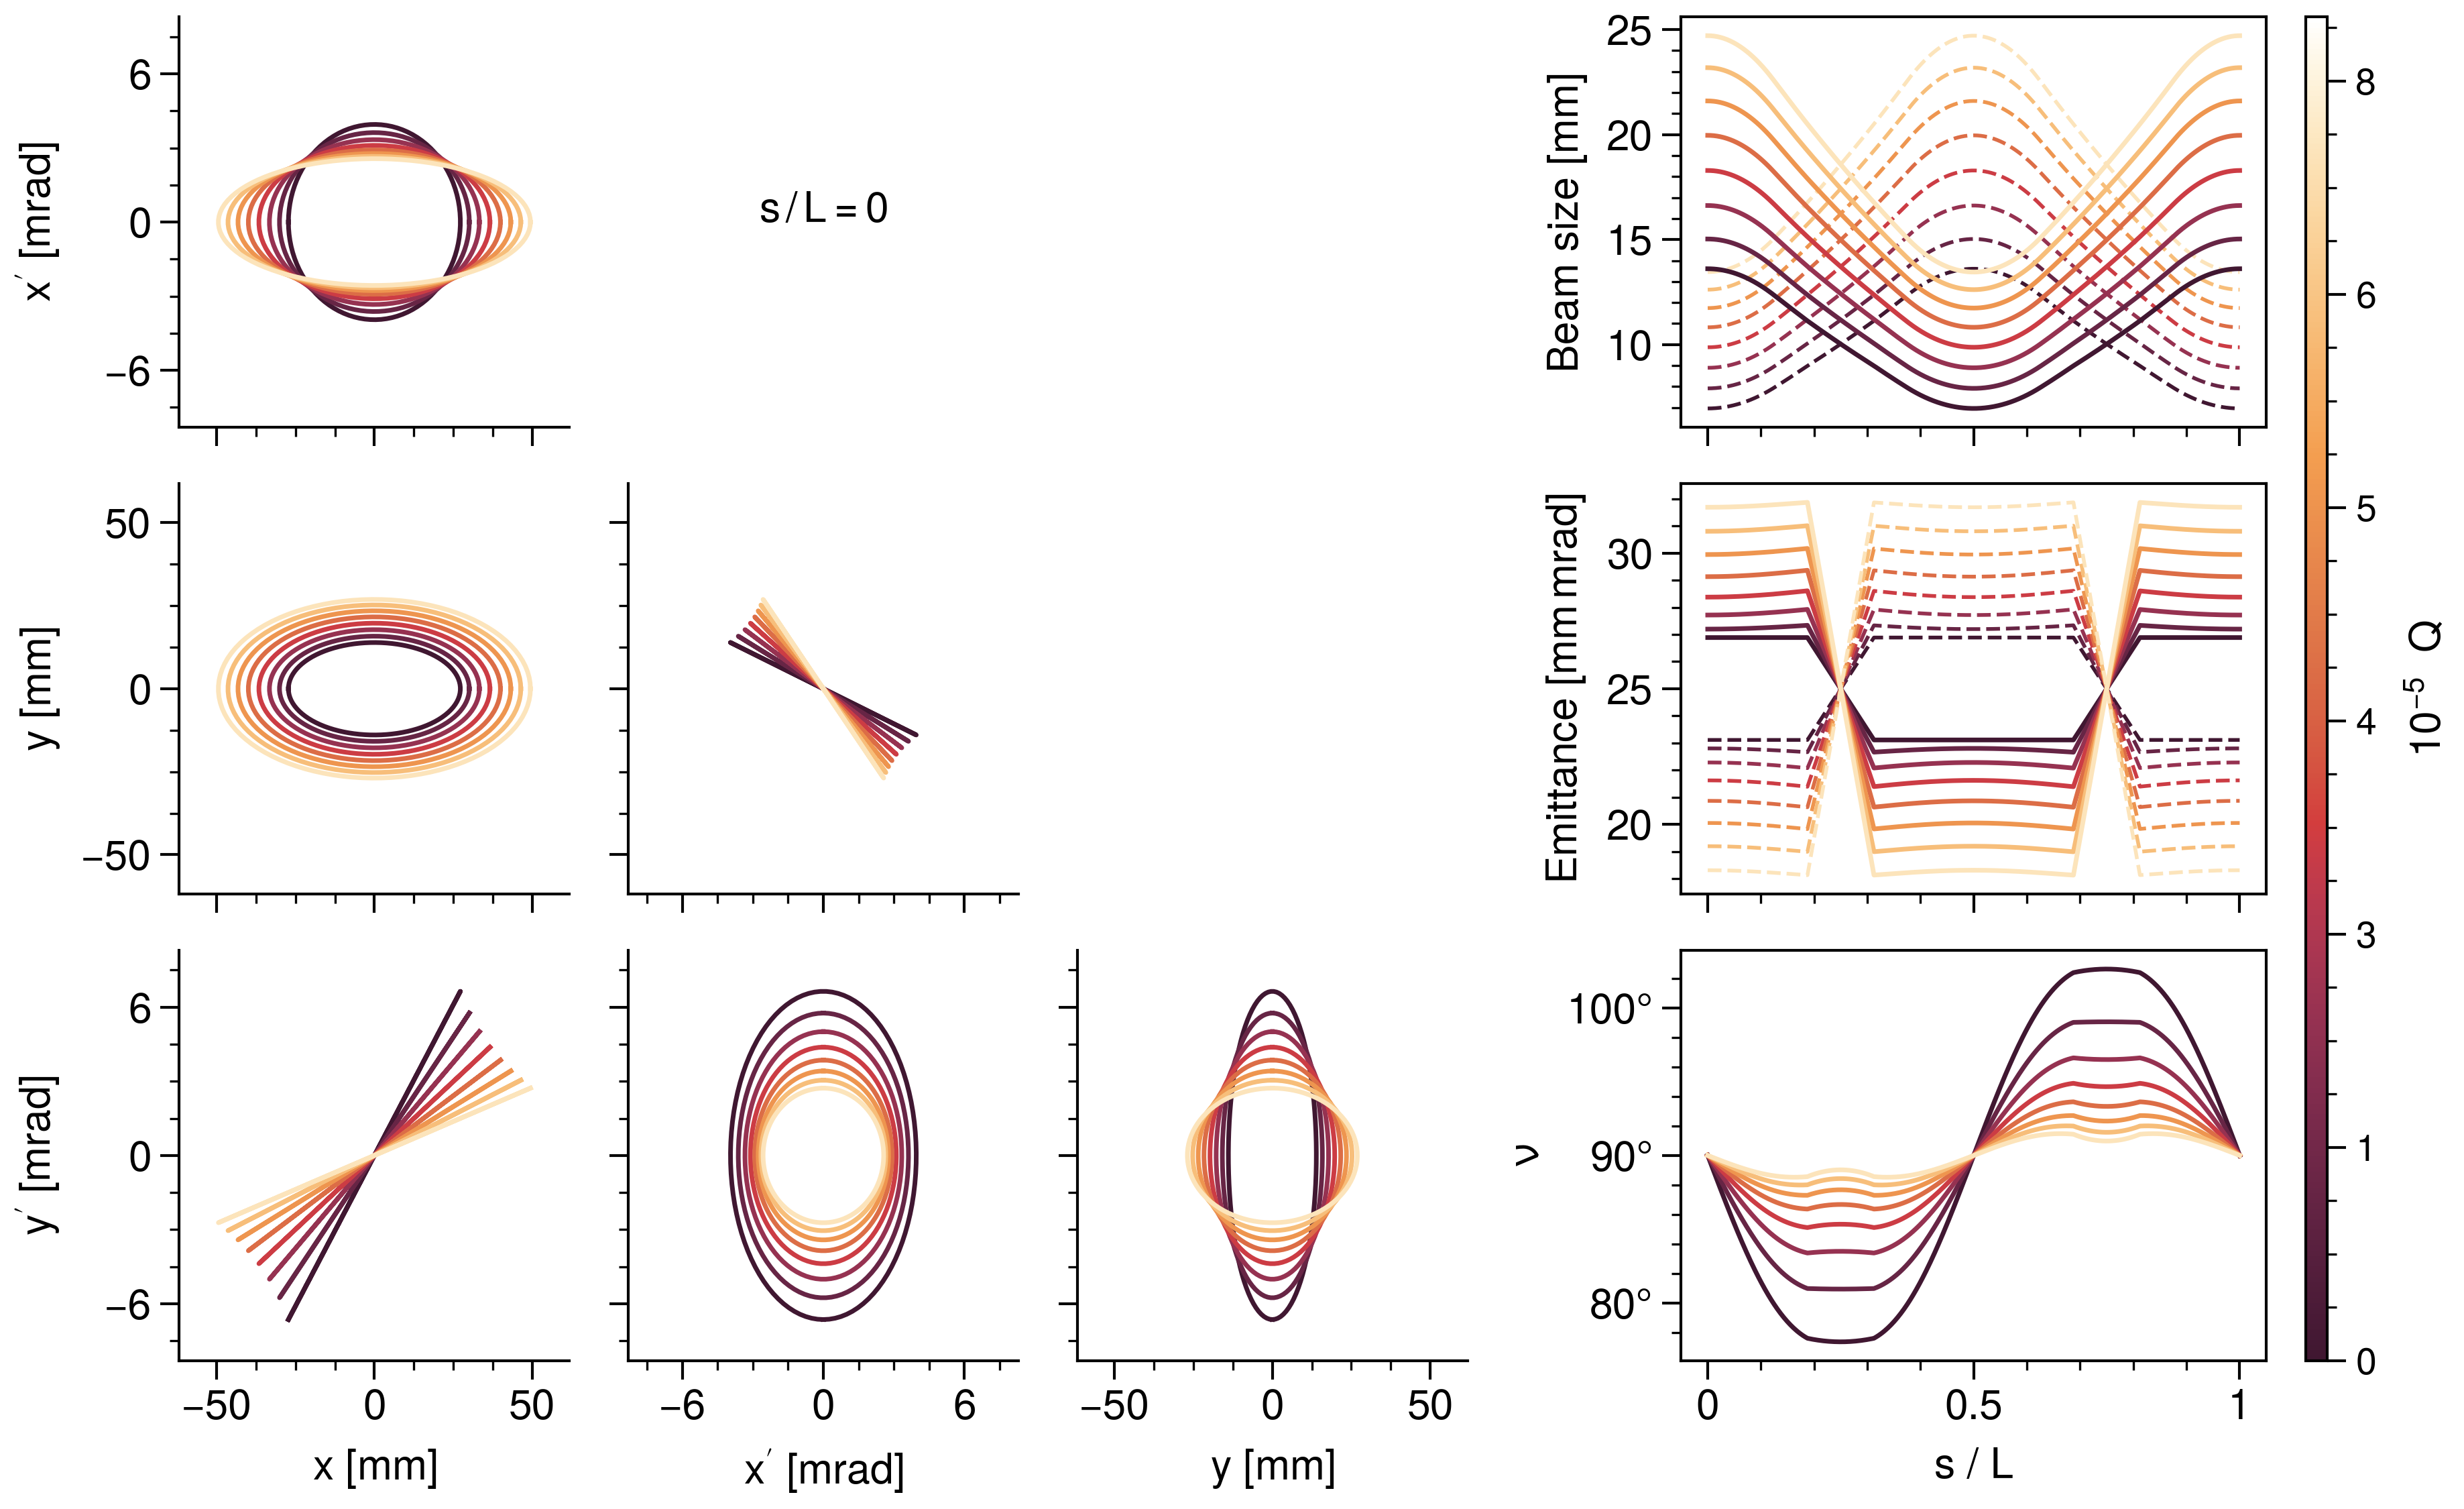
\includegraphics[width=\textwidth]{Images/chapter2/matched_vs_sc_fodo_sol_mode1.png}
        \caption{Solution 1}
        \label{fig:matched_vs_sc_fodo_sol_a}
    \end{subfigure}
    \vfill
    % \vspace*{1.0cm}
    \vfill
    \begin{subfigure}{1.0\textwidth}
        \centering
        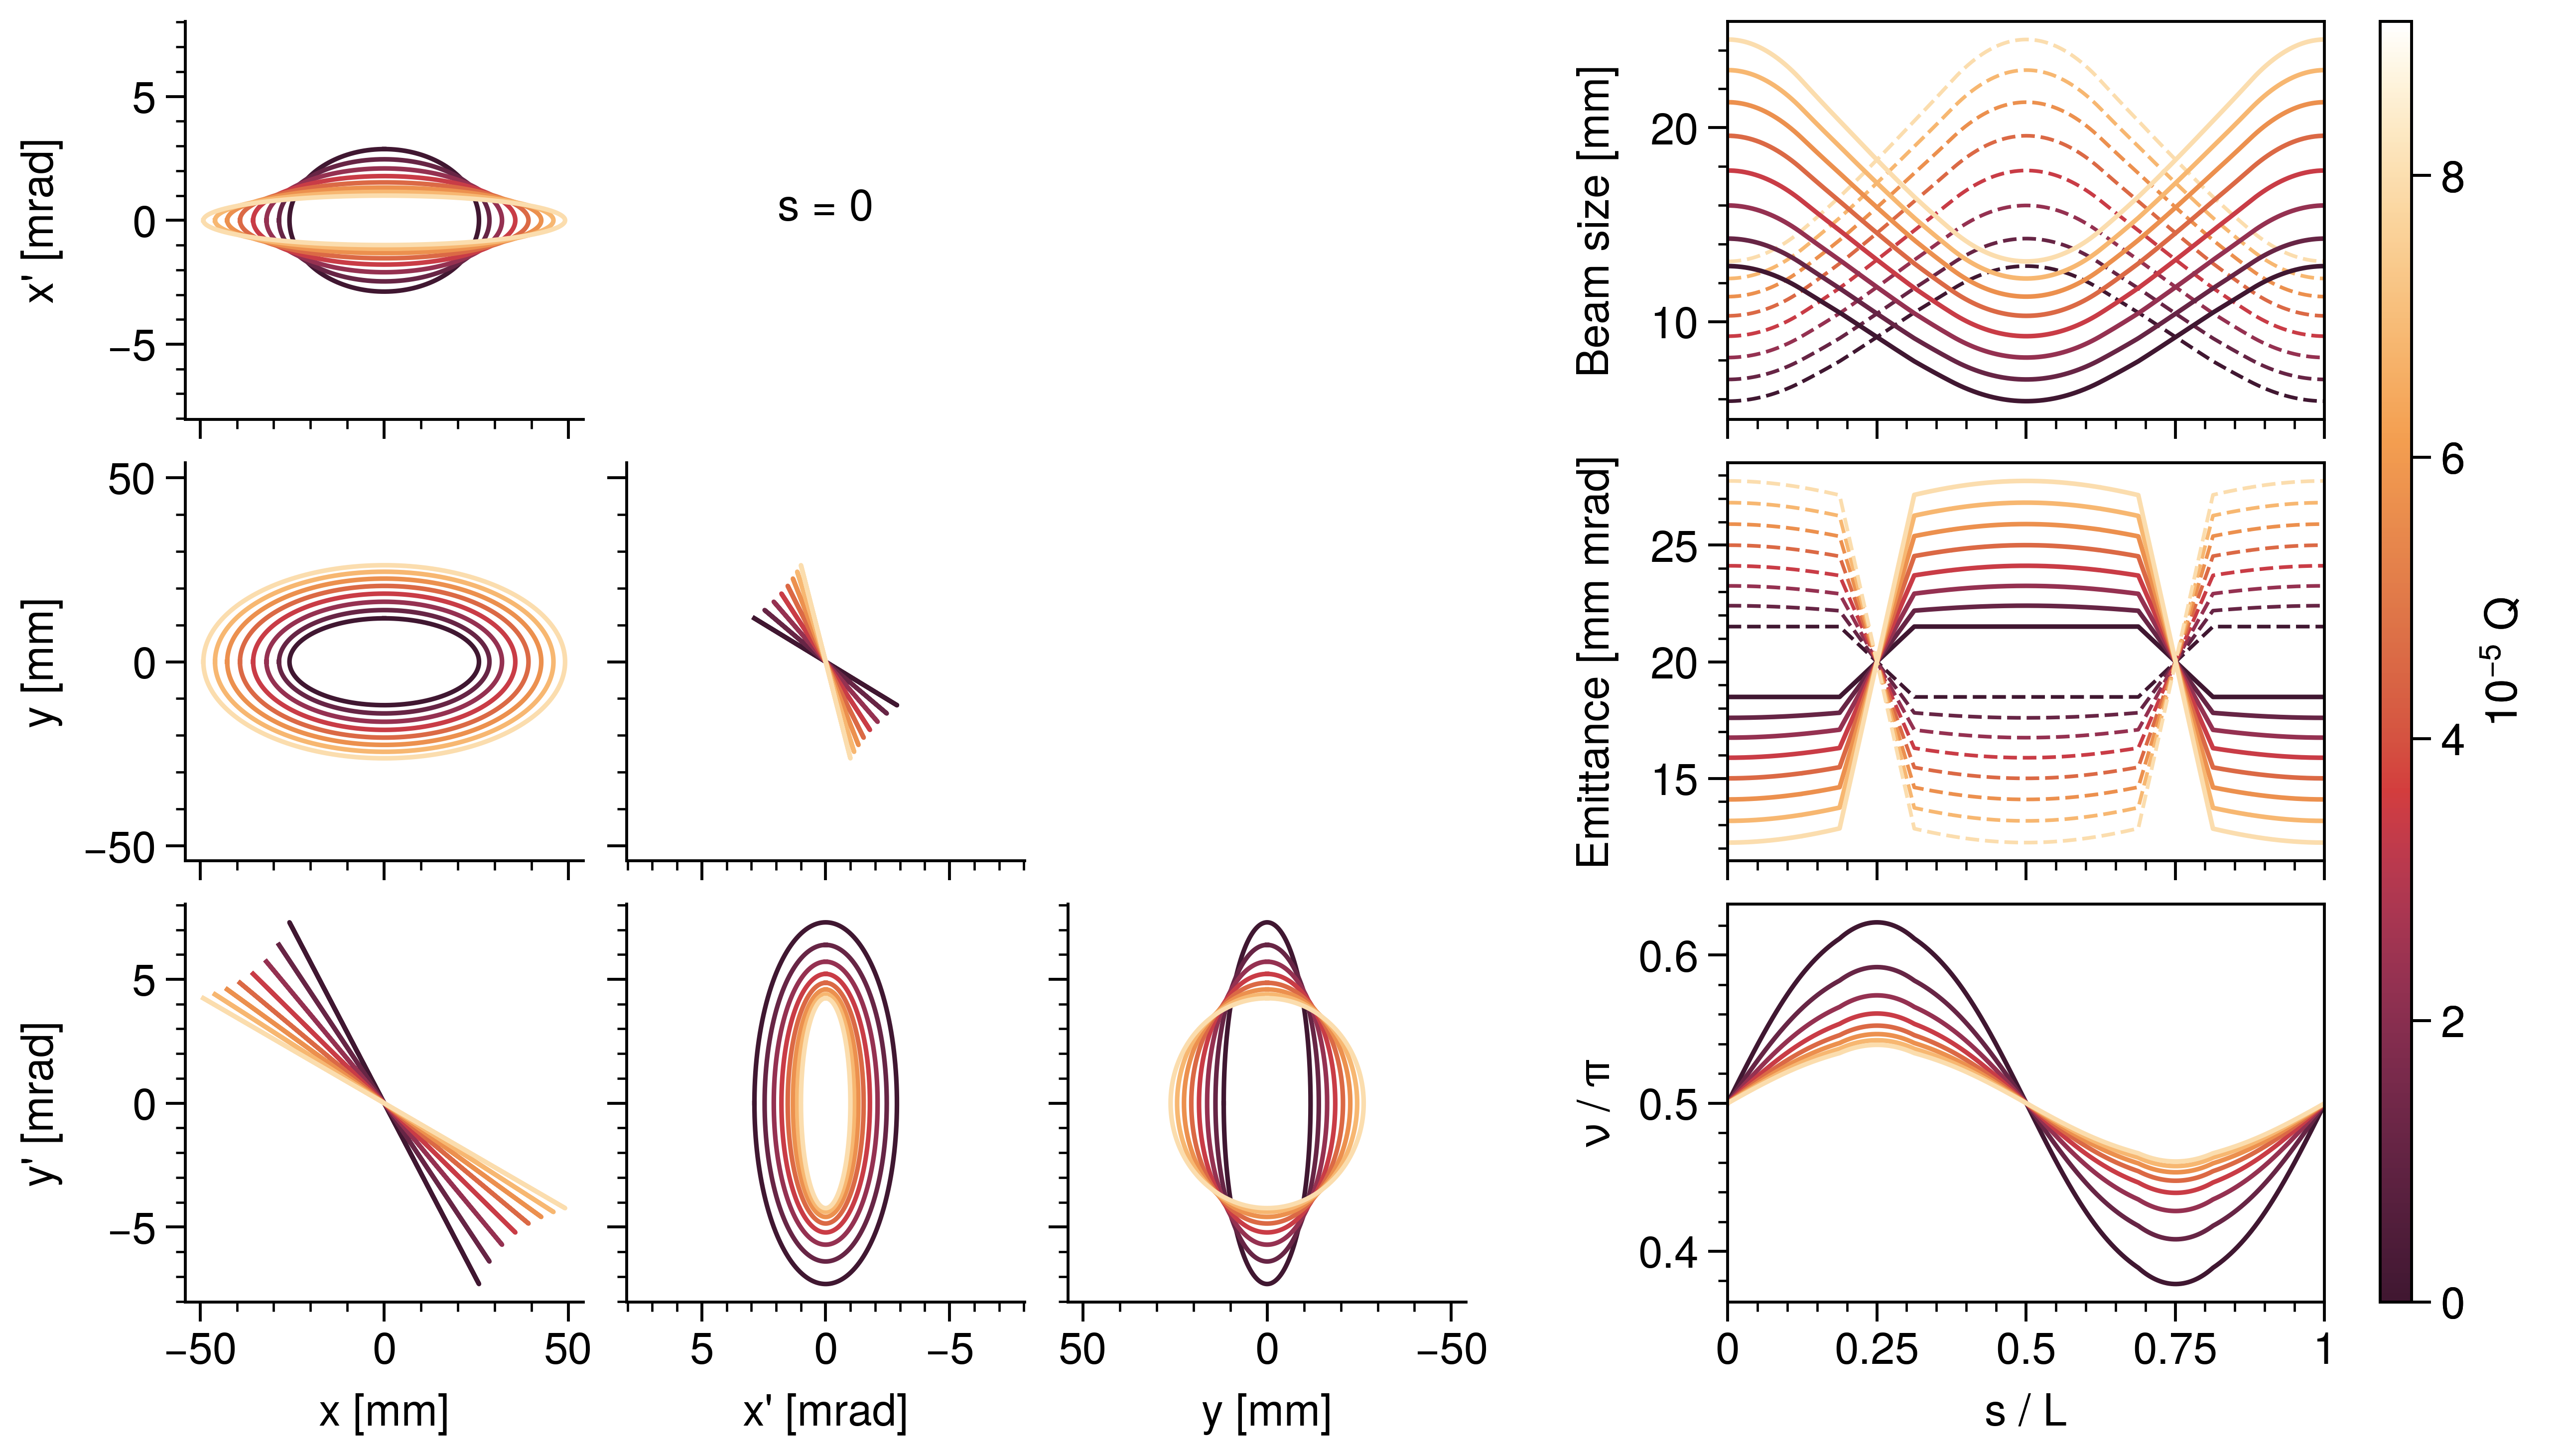
\includegraphics[width=\textwidth]{Images/chapter2/matched_vs_sc_fodo_sol_mode2.png}
        \caption{Solution 2}
        \label{fig:matched_vs_sc_fodo_sol_b}
    \end{subfigure}
    \caption{Matched envelope of the Danilov distribution in a coupled FODO lattice as space  charge is increased. The lattice is coupled due to solenoid magnets inserted between the quadrupoles. Left: phase space projections at the lattice entrance. Right: beam parameters within the lattice. Solid lines are for $x$ and dashed lines are for $y$ in the top two plots.}
    \label{fig:matched_vs_sc_fodo_sol}
\end{figure}
%
The matched beam resembles that of the uncoupled FODO lattice in Fig.~\ref{fig:matched_vs_sc_fodo}; most notably, it is round at the symmetry points in the lattice. The differences are found in the apparent emittances: their oscillation amplitude is larger within the drift spaces and quadrupoles, and there is a significant additional emittance exchange within the solenoids. 


\subsubsection{Effective transfer matrices}

The effective transfer matrix generated by the lattice and matched beam can be calculated by tracking test particles subject to the internal fields of the matched beam. It is important to note that in each case the matched beam is a function of one of the transfer matrix eigenvectors; the second eigenvector does not necessarily correspond to a matched solution in the same lattice. For example, in the uncoupled FODO lattice, the solutions share the same effective transfer matrix. In the coupled skew quadrupole lattice, the two solutions do not share the same effective transfer matrix. In the latter case, the unused eigenvector is a matched solution for a lattice in which the sign of all skew terms is reversed (a mirror reflection in one plane). 

The eigenvalues of each effective transfer matrix are plotted in the complex plane as space charge is increased in Fig.~\ref{fig:effective_transfer_matrix_eigvals}; the corresponding phase advances are also printed.
%
\begin{figure}[!p]
    \centering
    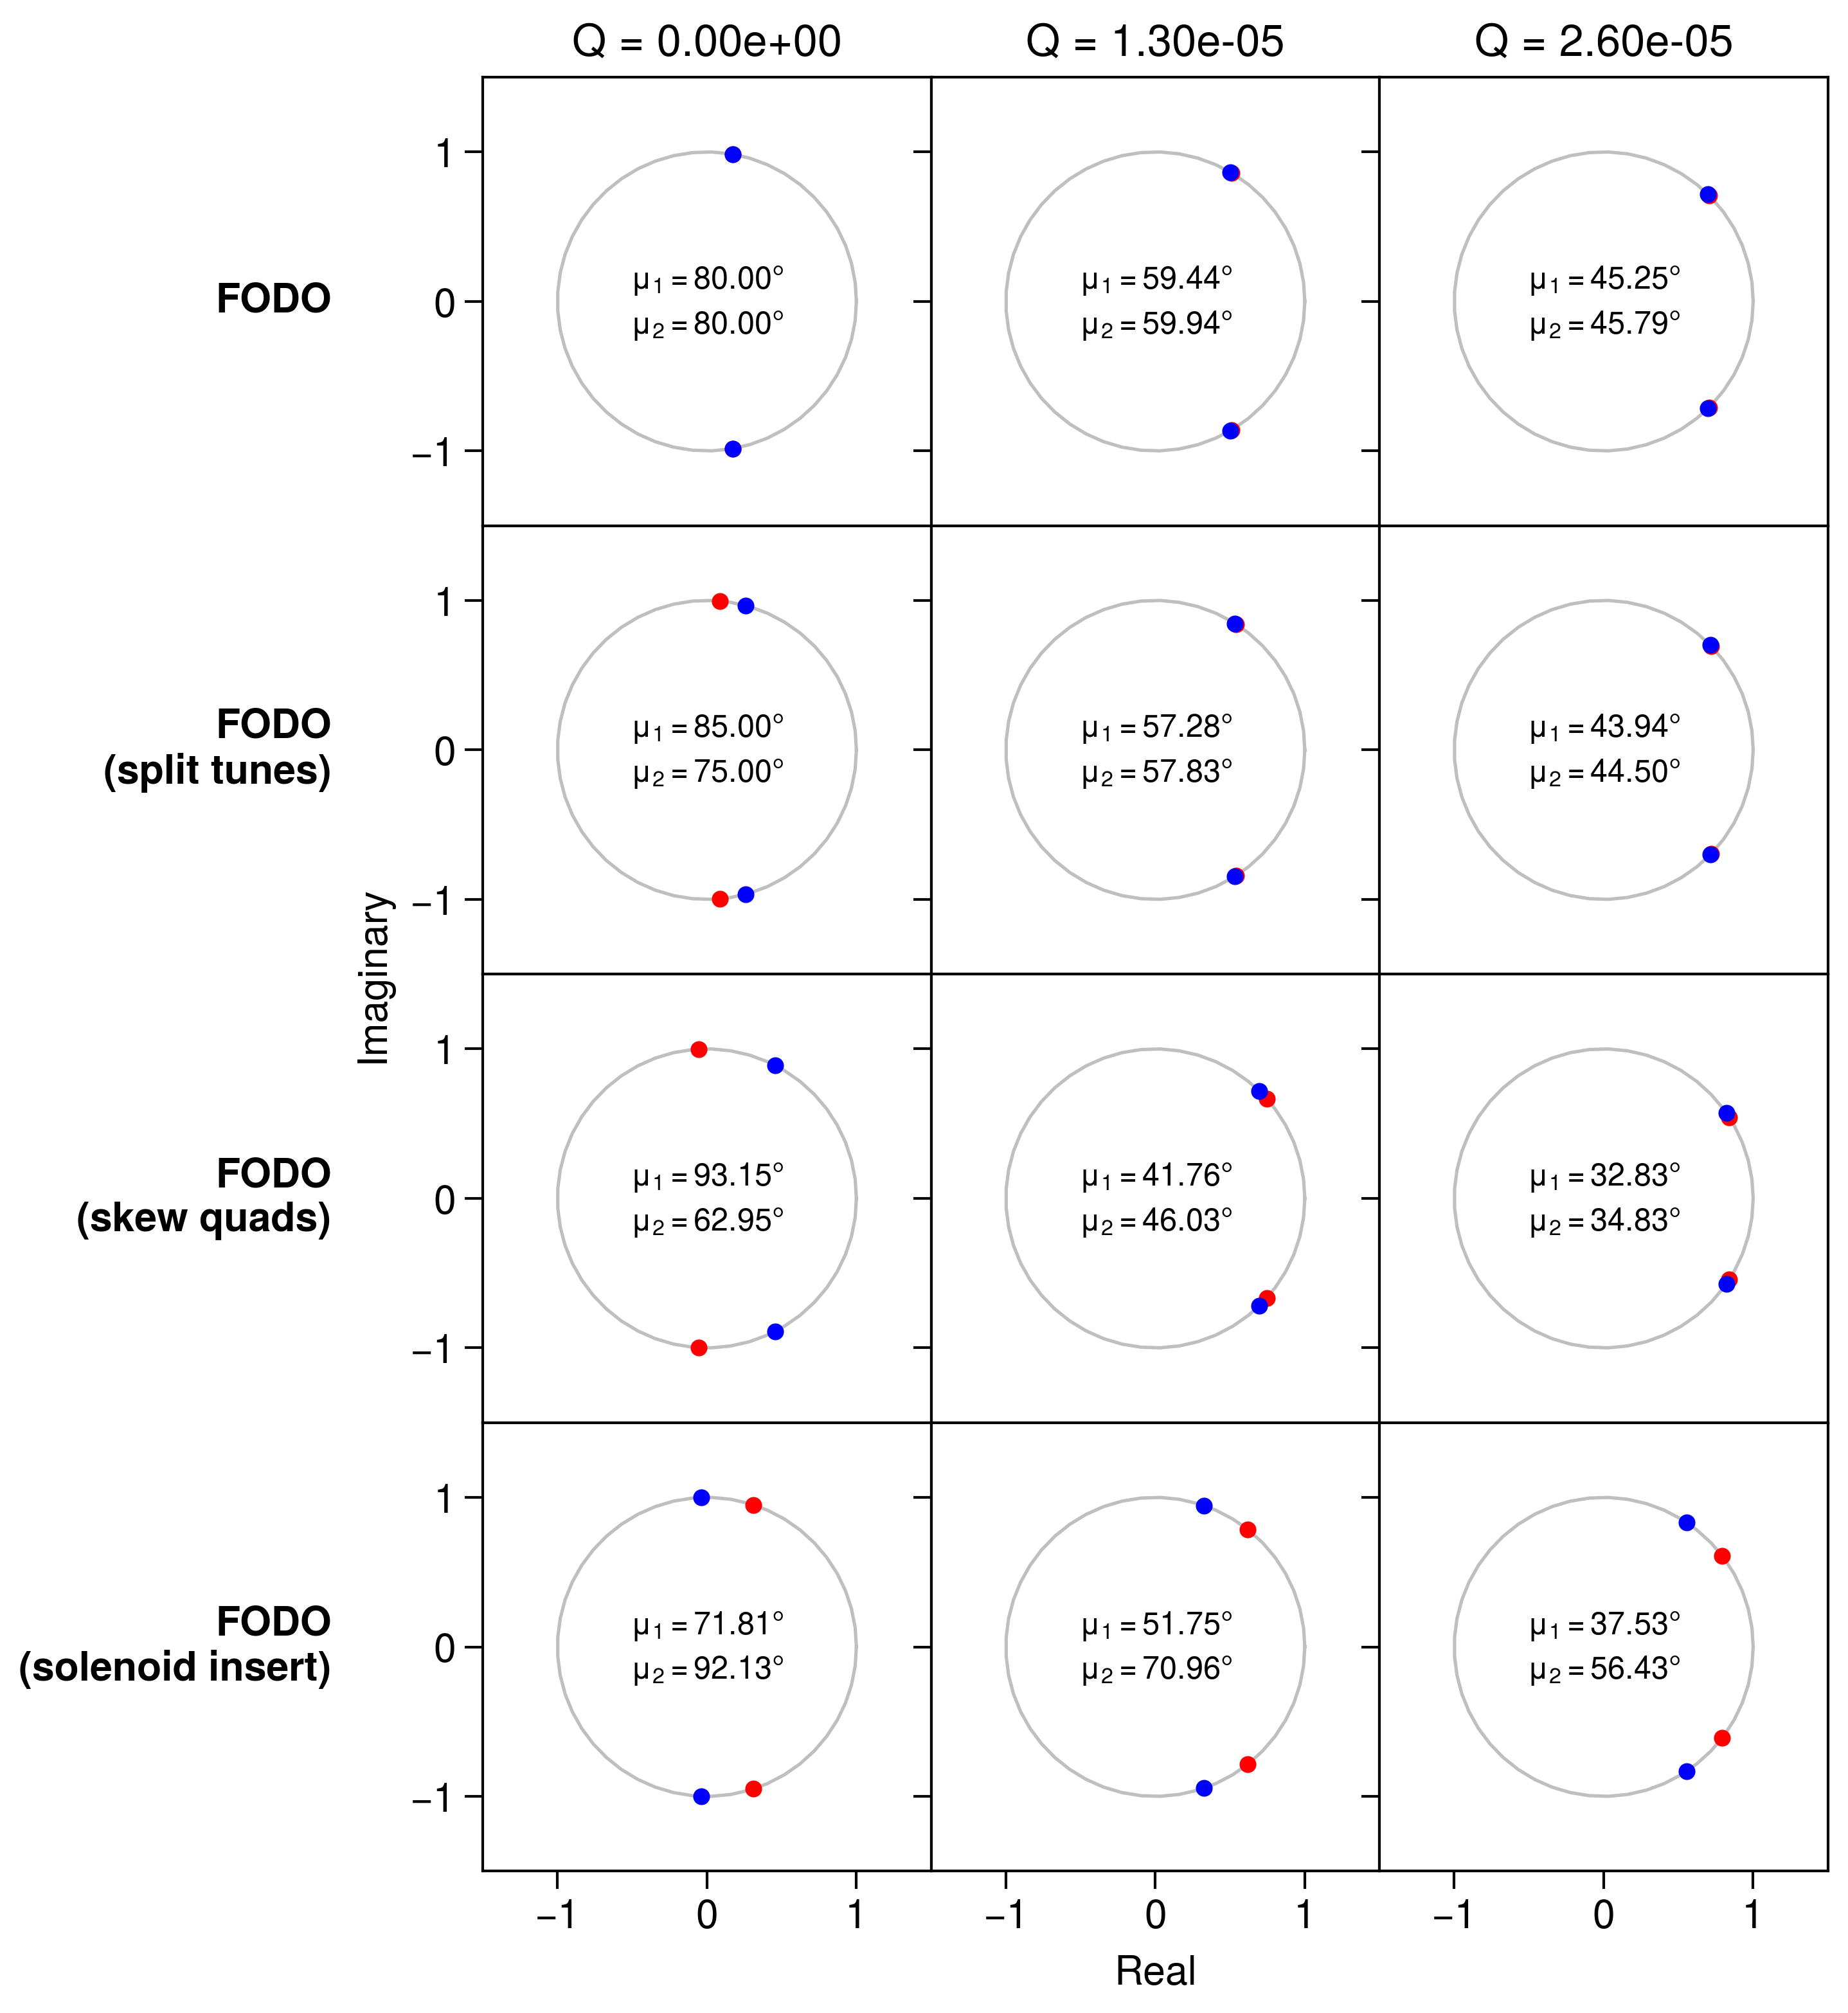
\includegraphics[width=\textwidth]{Images/chapter2/eigvals.png}
    \caption{Eigenvalues of the transfer matrix of the effective lattice generated by the matched beam, plotted in the complex plane.}
    \label{fig:effective_transfer_matrix_eigvals}
\end{figure}
%
We observe that the difference between the phase advances $\Delta = |\mu_2 - \mu_1|$, which is a measure of the coupling strength in the effective lattice, is never zero when space charge is nonzero. (In the top two rows, $\Delta$ is very small and the plotted eigenvalues lie nearly on top of one another.) We also observe that the matched beam space charge ``cancels out" some of the bare lattice coupling; for example, in the skew quadrupole lattice $\Delta$ is large in the left column (zero space charge) but nearly zero in the far right column. This is not true when coupling is included through the insertion of solenoid magnets; $\Delta$ instead remains relatively constant.  


\subsection{Relevance to experiment}

These envelope studies pave the way for future research on the stability of the Danilov distribution using perturbations around the matched envelope \cite{Goswami2016}, as well as halo formation using the particle-core model \cite{Wangler1998, Gluckstern1994, Gluckstern1998}. Our findings are also relevant to experiments that seek to create a Danilov distribution in the SNS ring using phase space painting. Theoretically, elliptical painting is optimized if the matched envelope is computed first; painting then proceeds along the eigenvector of the effective transfer matrix generated by the matched beam. 

Holmes et al performed PIC simulations to determine the feasibility of elliptical painting in the SNS \cite{Holmes2018}. These simulations are described in more detail in Chapter \ref{chap-3}; for now, we mention a few findings:

\begin{quote}
    \textbf{Finding 1}: The ideal painting path in the SNS is a line in the $x$-$y'$ plane.
\end{quote}

\noindent{The reasoning in \cite{Holmes2018} is that, due to the geometry of the injection region, variation of $x'$ during injection leads to scrapping losses. We have found another reason why this painting path is ideal: in general, the matched solution with space charge at a symmetry point ($\alpha_x = \alpha_y = 0$) in an uncoupled lattice is upright; i.e., $\nu \approx \pi/2$. The injection point in the SNS ring has $\beta_x \approx \beta_y$ and $\alpha_x \approx \alpha_y = 0$, so this general principle should apply. And it does; Fig.~\ref{fig:matched_env_SNS} shows the matched envelope at the SNS injection point with realistic beam parameters: $\varepsilon_2 = 20$ mm mrad, energy = 0.8 GeV, bunch length $\approx$ 3/4 ring length, and intensity = $0.75 \times 10^{14}$.
%
\begin{figure}[!p]
    \centering
    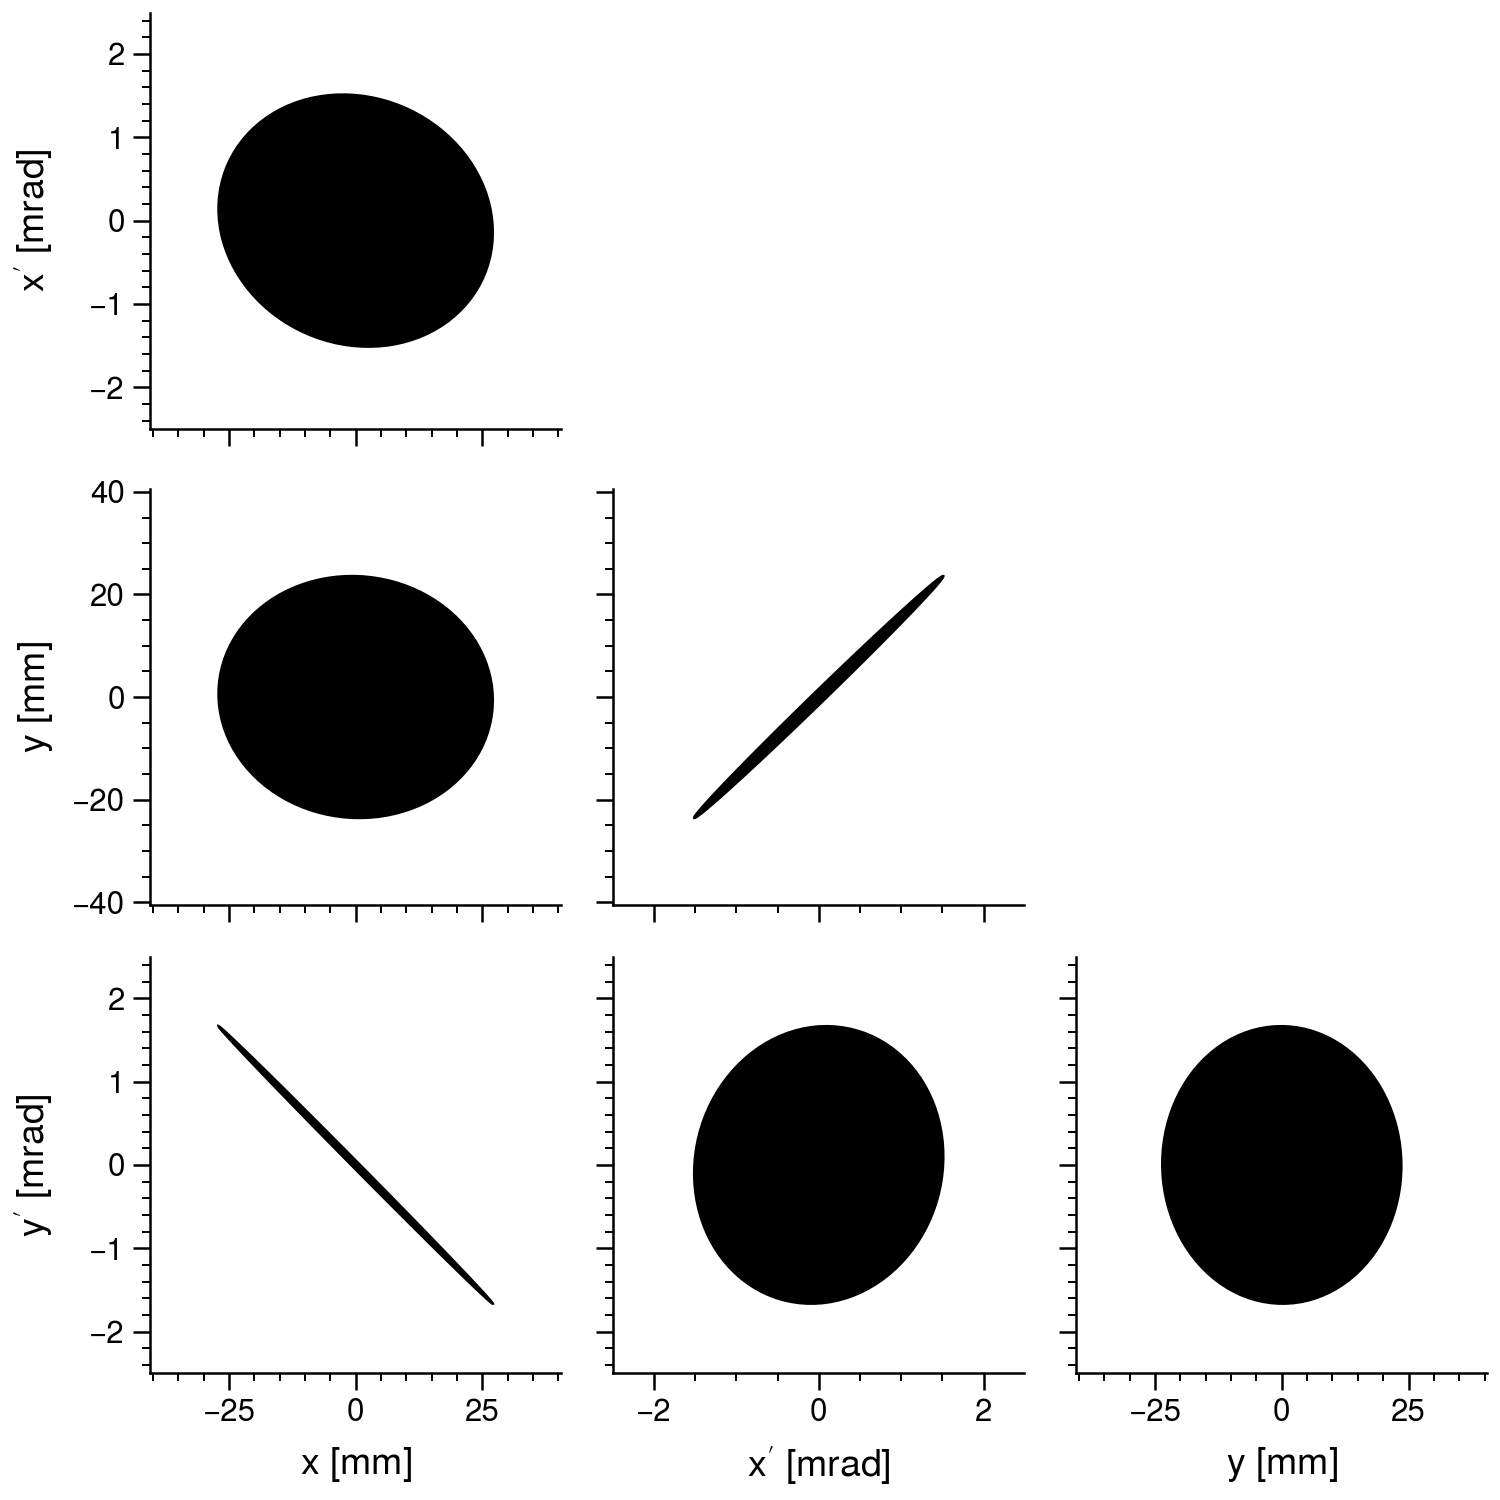
\includegraphics[width=0.8\textwidth]{Images/chapter2/matched_env_SNS.png}
    \caption{Matched beam envelope at the SNS injection point. Parameters: $\varepsilon_1 = 0$, $\varepsilon_2 = 20$ mm~mrad, energy = 0.8 GeV, intensity = $0.75 \times 10^{14}$, bunch length $\approx$ 3/4 ring length.}
    \label{fig:matched_env_SNS}
\end{figure}
%
Variation of $\nu$ has the potential to generate large mismatch oscillations due to the linear coupling from the beam. During painting, this means that the ideal cross-plane correlations will at least be blurred. It is also likely that the uniform density ellipse will not be maintained since particles will not be injected onto the edge of an invariant ellipse. In Fig.~\ref{fig:mismatched_env_SNS}, the same beam as in Fig.~\ref{fig:matched_env_SNS} is tracked, but the $\nu$ parameter is changed by $\pi / 4$. 
%
\begin{figure}[!p]
    \centering
    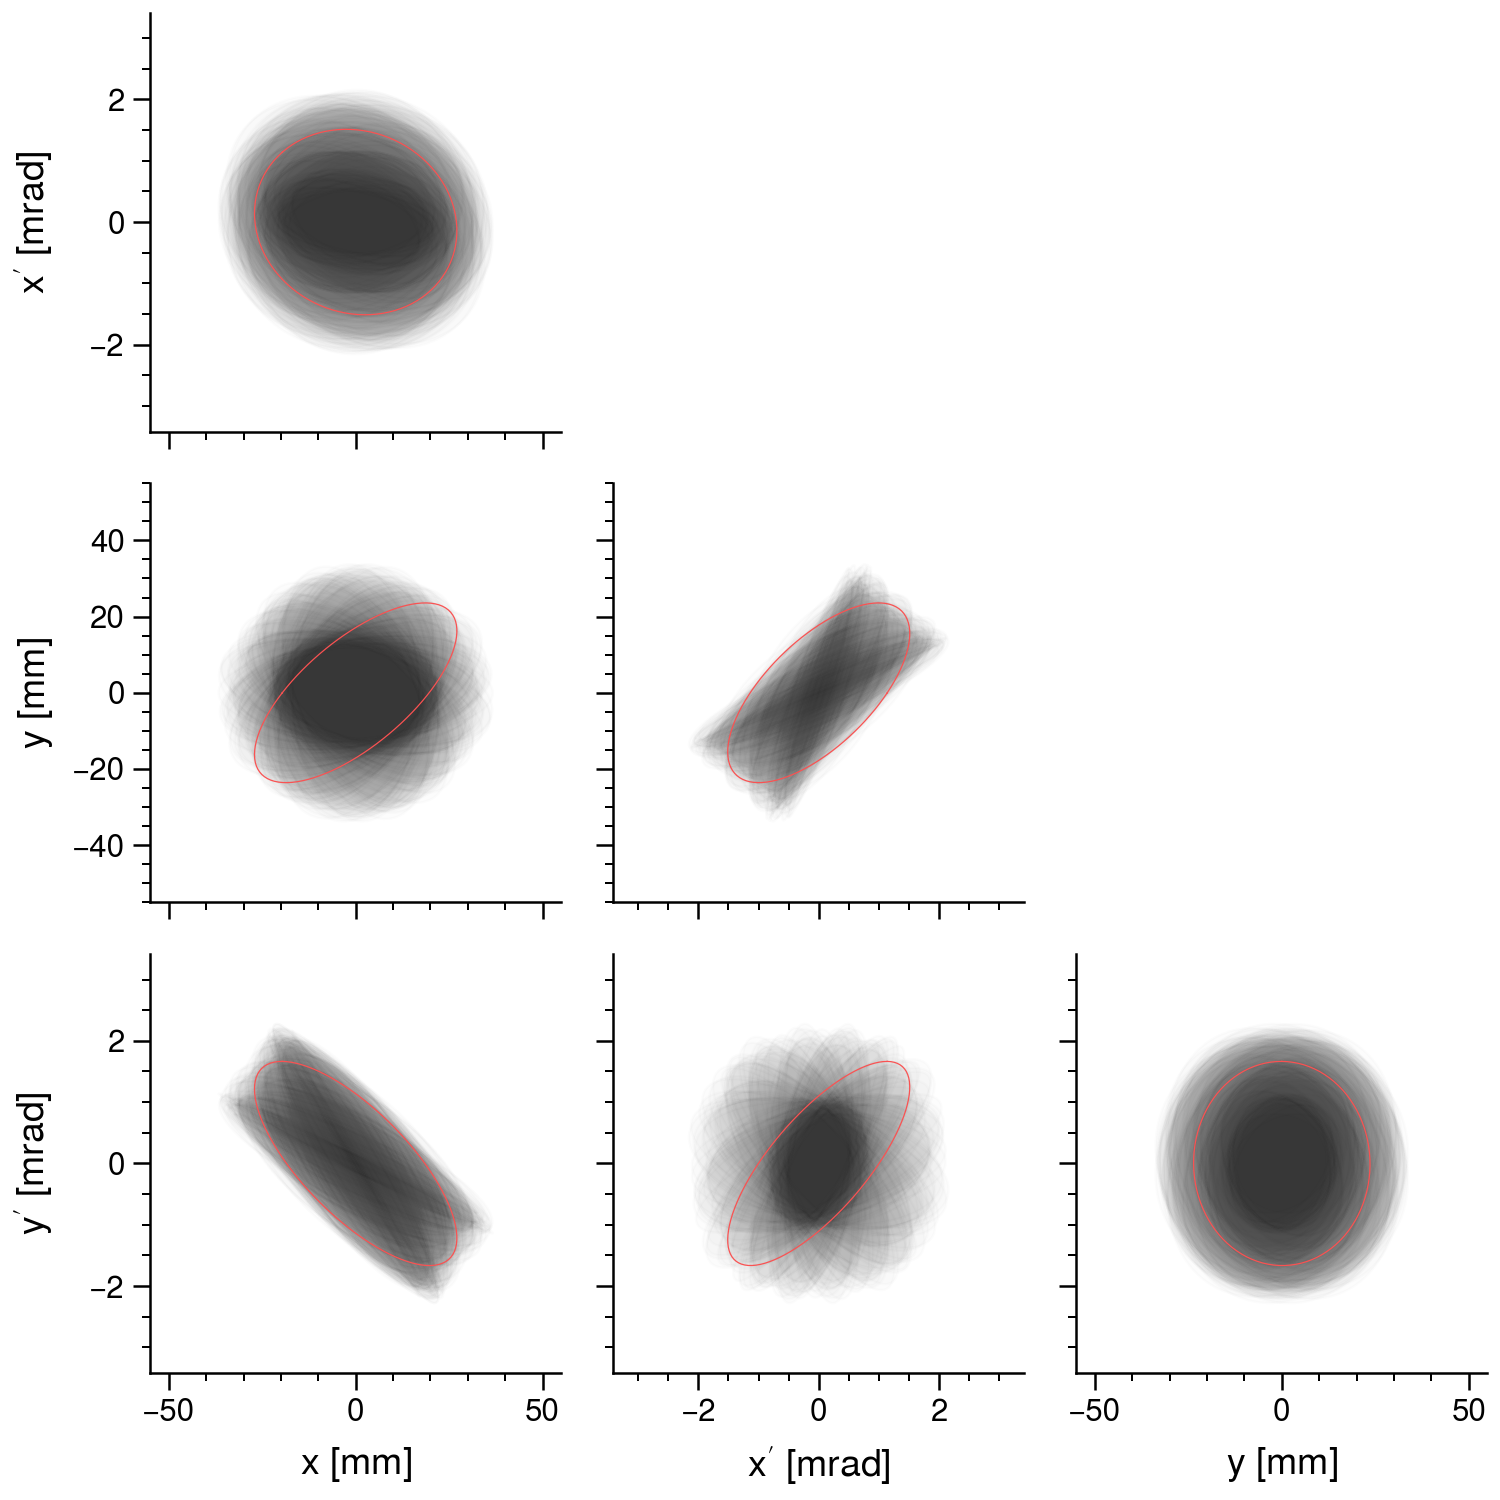
\includegraphics[width=0.8\textwidth]{Images/chapter2/mismatched_env_SNS.png}
    \caption{Mismatched beam envelope at the SNS injection point. The parameters are the same as in Fig.~\ref{fig:matched_env_SNS}. The red ellipse is the initial beam, and black ellipses show 100 subsequent turns overlayed on the same plot.}
    \label{fig:mismatched_env_SNS}
\end{figure}
%
The red line shows the initial beam; the beam ellipses over the next 100 turns are overlayed on the same plot. The mismatch causes a large space-charge-driven emittance exchange, causing the beam to rotate turn-by-turn and blur the $x$-$y'$ correlation. The superposition of these ellipses is no longer self-consistent. 
}
% Something about [less room for error when the beam is skinny].


\begin{quote}
    \textbf{Finding 2}: The final beam quality in an uncoupled lattice is, to a degree, insensitive to the tune split $\nu_x - \nu_y$ when space charge is included.
\end{quote}

\noindent{
The reasoning in \cite{Holmes2018} is that the beam adjusts its shape such that the depressed horizontal and vertical tunes are equal. We have confirmed this using the envelope model and a simple lattice. It is possible to find a matched beam even for a significant tune split: the horizontal and vertical emittances adjust to produce an asymmetric tune depression between the horizontal and vertical planes. Operating at equal tunes is necessary for elliptical painting in an uncoupled ring; it is worth exploring whether a slight tune split can be compensated by changing the ratio of painted $x$ and $y$ emittances.}


% \begin{quote}
%     textbf{Finding 3}: Solenoid magnetic fields stabilize the beam against nonlinearities.
% \end{quote}

% The reasoning in \cite{Holmes2018} is that nonlinear coupling from fringe fields is enhanced at the difference resonance $\nu_x - \nu_y = 0$, and that the solenoid splits the particle tunes. We have found another reason why a solenoid is beneficial: the solenoid helps maintain a round beam. 

% [...]

Finally, a yet-unconsidered modification to the SNS is to turn on the skew quadrupole correctors in the ring. It would be ideal to avoid the large transverse momentum kicks required to paint a rotating beam, which introduces technical challenges as well as opportunities for beam loss, and instead, vary only the relative positions of the injected and circulating beams. It is thus worth exploring whether skew quadrupoles can be used to change the shape of the matched beam so that the required angular kick is minimized.


\subsection{Summary}

The evolution of the Danilov distribution is given by its envelope equations. An iterative procedure to calculate the matched envelope was developed by observing that the matched beam is a function of a single eigenvector of an unknown, linear, coupled lattice. 

The method was demonstrated in a simple FODO lattice, which was then modified to study the effects of unequal tunes and linear coupling. Two matched solutions, one for each choice of intrinsic emittance, were obtained for each lattice and beam perveance. The primary difference between these two solutions was found in the sign of their angular momentum. A common finding among nearly all the cases was that the shape of the matched beam in phase space remained approximately the same as space charge was increased; the main effect of space charge was to increase the average beam area within the lattice, as well as to introduce an exchange of the horizontal and vertical emittances.

Several observations from simulations in \cite{Holmes2018} were illuminated by these studies. In particular, by computing the matched beam envelope at the SNS injection point, further justification was given to the choice of the $x$-$y'$ painting path.
